% !TeX program = LuaLaTeX

\documentclass[10pt,a4paper,twocolumn,openany]{book}

%%% Loading the main rpg-book style
% Options: bg-a4, bg-letter, bg-full, bg-print, bg-none. This changes the background used.
\usepackage[bg=none]{lib/rpg-book} 

\begin{document}

%----------------- Text begins here -----------------% 
%% It is distributed in several files.

%% NOTE : use \include to skip a page, and \input to simply transpose the contents of the file at this position.
%% If this is only a section, it might be more relevant to use \input

%% NOTE: if you get a weird "begin \command ended by \othercommand" error, 
% it likely means you have opened quote marks (") or brackets ({) that do not have a corresponding closing quote mark or bracket.

% TITLE
\begin{titlepage}

	% Background parchment
	\thiswatermark{\centering \put(-200,-900) {
\includegraphics[angle=0, scale=1]{img/background.jpg}} }    
	
	\begin{center}
		\bfseries

		\vspace*{2.25cm}
		
		{\color{title1} \Huge D\fauxsc{reamshard}}
		\vskip0.5cm
		
		
\includegraphics[width=.45\paperwidth]{img/separator.png}
		\vskip1cm

		\Large A Role-Playing Game Rulebook
		\vskip1cm
	\end{center}
	
	\vskip4.5cm


	% Logo
	\begin{center}
		
\includegraphics[width=122bp,height=78bp]{img/rising_vergina_sun.png}
	\end{center}

	\vskip1cm

	% Blurb
	\centerline{

		\begin{minipage}{.6\textwidth}

			A Role-Playing Game system derived from the \textit{d20} framework, with its accompanying Lore. It uses a flexible classless system, with different degrees of success for the outcomes of rolls. \\

			\vskip0.2cm

			This is set in a low-fantasy late medieval universe, on the Dreamshard Archipelago, which was recently shaken by unexplained magical phenomena. This is compounded by an unstable geopolitical situation, in which powerful Magisters vie for influence. \\
			
			\vskip0.2cm

			The players are mandated by the Imperial governor to investigate reports of activity from the fabled Voskari. What will you find, and should it have stayed in the shadows? \\

			\vskip0.3cm

			\textit{Open Creative Commons - BY license}

		\end{minipage}
	}
	
	\vskip2cm
	
	\hfill
	\begin{flushright}
		\Large \textbf{by Quentin Ferré}
	\end{flushright}

\end{titlepage}




\tableofcontents

% Foreword and acknowledgements
\addcontentsline{toc}{chapter}{Foreword}
\chapter*{Foreword}

Welcome to the rules for the \textit{Dreamshard RPG}!

My goals in this project were to create a system that had simple rules, but a lot of gameplay depth. I wanted to let the players break free of traditional, class-based system, and instead give a lot of flexibility to both the GM and the players. As such, Characters instead draw from Ability trees than can be mixed and matched. As such, the system also permits a lot of Spell customization, and the design of custom Gadgets. 

I also wanted to diminish the "dump stat" effect, by making every Characteristing potentially relevant. The use of a roll system with degrees of success (and the presence of partial successes called "Grazes") also significantly reduces random misses, resulting in lower variance of outcomes. During playtests, I found this resulted in a more consistent gameplay experience, and crucially makes gameplay a lot faster.

The current version, however, has its drawbacks. The system relies a lot on adjudication by the GM, in particular for the design and balancing of the Tools, Abilities and Spells to give the players. I hope the guidelines provided in the Balancing section can help alleviate this.

Finally, this entire project was an excuse to do some worldbuilding, which as any Game Master ultra-nerd will tell you, is always one of the best parts. I hope you will enjoy the results, and above all, \textbf{have fun!}



\addcontentsline{toc}{section}{Acknowledgements}
\section*{Acknowledgements}

I wish to thank the members of my gaming group for helping me beta-test this system. In alphabetical order: Jeanne Chèneby, Laurent Hannouche, Adrien Long, Justine Long an Florian Rosier. In particular, special thanks to Jeanne for her copious feedback on the manuscript and the design of the rules themselves.

Also thanks to the designers of the Pillars of Eternity paper RPG, which was a huge inspiration.

The LaTeX template used in this manuscrit is a derivation the one designed by \textit{evanbergeron}. The font used, Souvenir, is used as a non-commercial application.

\vskip 0.5cm

This work is made under an open \textit{Creative Commons-BY} license. This version of the manuscript was compiled on January 1st, 2023.

Contact: \textit{quentin.q.ferre@gmail.com}



\paragraph{Art Credits}

In no particular order: Arnold Böcklin, Patrick O'Brien, Dariusz Zawadzki, Bob Ross, Mosè Bianchi, Dominique Van den Broech, Roland Davies, David and Nansi Gallup, Poulsen, Wonderdraft.


%% By file name :
% naval = Battle of the Chesapeake (Patrick O'Brien)
% machine head = Dariusz Zawadzki
% Island = bob ross
% death whisper = Self-Portrait with Death Playing the Fiddle (Arnold Böcklin)
% dark nun = Monaca di Monza, by Mosè Bianchi
% fort = Dominique Van den Broech
% galleon = roland davies
% kelp = David and Nansi Gallup
% port first choice = Poulsen

% Core rules
\chapter{Core rules}

The core gameplay loop of the Dreamshard RPG will be familiar to every tabletop RPG player. First, the Game Master (GM) describes the current situation, then the Players each describe what they want their respective Player Characters (PC) to do. Following this, the GM adjudicates: they decide if this is possible, and give the odds for a roll to determine the outcome if they so wish. Finally, the GM narrates the results. 

Whenever the rules are unclear, use common sense and personal preference. In any case, \textbf{the GM is always right}, and has full latitude to modify the rules to fit the situation. When a specific rule (such as an Ability) contradicts a general rule, the specific rule wins. Finally, when halving numbers, \textbf{round down} unless specified otherwise. 


\section{Dice rolls}
\label{dice_rolls}

Dice rolls should be used when the outcome of a given action is \textbf{uncertain}. For instance, for difficult tasks, or when there is a time constraint.

First, some terminology: an \textit{Actor} designates any agent in the game that is capable of taking Actions, be it a Player Character of a Non Player Character. Whenever an Actor tries to do something, if the GM calls for a roll, then the Actor will roll their \textit{Aptitude} against a given \textit{Difficulty}. In combat, Aptitude and Difficulty are respectively called an Accuracy and a Defense.

To do a roll, follow these steps:

\begin{enumerate}
    \item The GM picks the associated Characteristic modifier (see section \ref{characteristics}), and a Skill modifier (see section \ref{skills}) if applicable. 
    \item Furthermore, the GM may order additional circumstance modifiers, including but not limited to: Special Skills, environmental modifiers, etc.
	\item The GM determines and announces the Difficulty of the test.
    \item The player may present an argument to the GM for more modifiers, of for the use of different ones from the character sheet. \textit{Regardless, the GM always has the last word.}
    \item Roll the twenty-sided die, and add the modifiers, so that the \textbf{final score = 1d20 roll + Aptitude – Difficulty}. The Aptitude is the sum of all modifiers used in all previous steps\footnote{Meaning: Aptitude = Characteristic modifier + Skill modifier + any other modifier.}.
    \item Compare the final score to Table \ref{success_roll} to determine the quality of the action's result.
\end{enumerate}


\begin{rpg-examplebox}
	In this book, rolls are written using the following syntax: "[Characteristic modifier + Skill modifier + other modifiers - Difficulty] roll".
\end{rpg-examplebox}


Let us consider an example: disarming a trap. The GM decides that the required Aptitude will be DEX + Crafting, and that the trap's Difficulty is -2. This will be written as a "[DEX + Crafting - 2] roll".

Now, let's say the Character's DEX and Crafting Skill are +3 and +2 respectively. This means the final modifier will be $3+2-2=3$ and the final roll will be 1d20+3 whose result will be compared to Table \ref{success_roll}.

The general philosophy of the system is to ask the players what they want to do, then work a suitable Difficulty for the roll (and maybe request the use of an Ability). The GM has full freedom to cap, or generally change, the modifiers applied to any given roll.

If players request a re-roll, they should have a very good reason to do so: perhaps having acquired new skills, tools, or information, or the action not being time sensitive. If the GM feels like it, this may come with a potential tradeoff of more severe failures...


\paragraph{Assistance} 

A friendly Actor can help another Actor perform an action. They can provide, as a bonus modifier, half their Aptitude for a maximum of +3. In combat, this is an Action (see section \ref{actions}). Several Actors can help, but this can only stack up to +4 in the general case.

\paragraph{No hurry} 

If there is no hurry, the GM may allow Actors to simply take 10 as the result of the dice (meaning the true final result will be equal to 10 + Aptitude - Difficulty) instead of rolling. In particulary lenient cases, such as when the players are in a calm environment with all necessary tools and all the time in the world, they may take 14 instead\footnote{Do recall that the GM decides the Difficulty, so they can essentially determine the final result in advance since by fixing the dice result, the resulting score will be known in advance.}. This is not recommended for spur-of-the-moment actions, like persuading someone, but permitted for certain skill checks such as general knowledge checks. This is also not recommended if you intentionally want there to be an uncertainty as to the result, such as in certain kinds of Crafting\footnote{Taking 14 is not recommended here, but taking 10 could be justifiable.}.

It goes without saying that this is entirely at the discretion of the GM. The GM may decide that, even if you have a lot of time ahead, the outcome of a given action still has a degree of randomness, and ask you to roll a dice regardless.


\subsection{Determining the Difficulty}
\label{difficulty}

The Difficulty to oppose a roll is usually equal to the appropriate Defense of the target: \textbf{Fortitude, Reflex or Will}. Those depend on the Characteristics of the target (plus, as always, any relevant modifier to them), and are detailed in section \ref{defenses}. 

Barring that, if no Defense is applicable, the \textbf{pseudo-Difficulty} can be calculated by taking the sum of all the relevant modifiers: usually the exact same modifiers that would be summed to calculate an Aptitude if the target was the one who was doing the action. If there is no target Actor, the GM will work out a Difficulty based on the odds they want to give to the players.

Let's make it more concrete: most social challenges will use a modulated Will as Difficulty. Most surprises would use Reflex, but sneaking would likely be opposed by the sentinel's equivalent Aptitude (WIT + maybe Discretion + circumstance modifiers). For all of this, please read section \ref{balancing_rolls} for more advice!

\begin{rpg-examplebox}
	Ultimately, the GM decides the Difficulty, no matter what the rules say!
\end{rpg-examplebox}

\paragraph{Angle of approach}

Beyond raw statistics, the angle of approach matters when determining the Difficulty. Consider social challenges, for instance. They should use a modulated Will; for example, Will-2 to convince someone of a trivial thing, but Will+4 for something they are loathe to do. Furthermore, if the player gives a very compelling in-character argument while roleplaying, or gives a very good piece of evidence, the Difficulty should be lower than if they give a bad argument, even with high Psychology. I recommend the modifiers applied to be about \textpm 2 for such cases, depending on the odds you want to give your players\footnote{For instance, if you want a PC to have 50\% odds of success (plus 25\% odds of only partial failure) set the Difficulty equal to the PC's Aptitude for the task.}. A similar argument can be made for other types of rolls.


\paragraph{Hidden Difficulty} 

In the general case, one always knows whether their roll succeeded or failed. However, the GM can always instead call for a roll but keep the Difficulty a secret, and consider the result themself, without announcing it explicitly to the player. 

This is best used when stating the real Difficulty would be a story spoiler, or when the player has no compelling logical reason to know exactly how likely they were to succeed, or whether they succeeded.

\subsection{Special dice rolls} 

In addition to the rules presented above, certain rolls may have additional rules.


\paragraph{Flipped rolls} 

Flipped rolls are called "flipped" because the target of the action executes the roll, instead of the Agent performing the action. Here, the Defense of the target is used as a (pseudo-)Aptitude for the roll.

These rolls are applicable when a player (or any Actor) is targeted by non-sentient hazards or opponents, such as traps, falling rocks, poison, a launched fireball, etc. because in this case, there is no "aggressor" Actor whose Aptitude can be used. For instance, if a trap or hazard of has a Difficulty of 3, the roll made by the Actor who triggers it to avoid its effect will be [Reflex - 3], with Reflex (normally a Defense) as the Aptitude.

This should be used sparingly, since the rolls results are biased towards succeeding (see table \ref{success_roll}) due to the possibility of Grazes. This means that simply flipping any roll (meaning switch Aptitude and Difficulty) increases the chances of success. As such, you may want to treat Grazes as failures, depending on the odds you want to give. 

Flipped rolls exist for player satisfaction reasons, because unlike in other d20 systems, there is no Challenge Rating to be matched. It may also be used when the attacker is sentient and attacking, as we don't want the player to feel like the GM rolled their dice instead of the player, behind their screen, and simply decided to bestow a calamity upon the PC. As a general recommendation, use regular rolls for standard actions but flipped rolls for the more potentially devastating ones.

As a general rule, any malus that gives "-X to all rolls" will also impact Flipped rolls, though the GM may decide otherwise.


\paragraph{Opposing rolls} 

Opposing rolls are used when two Actors are \textit{actively} opposing one another. For example, two people pushing against a door, or a pursuit with one party actively dodging. This is not recommended for simpler checks like convincing someone, or tripping them.

Each Actor makes a normal roll, and then the opponents compare their totals from step 5: that is to say the sum of the dice roll and all modifiers. Straightforwardly, the highest total wins. For the protracted contests that are longer or more impactful, such as long pursuits or high-stakes debates, see section \ref{protracted} instead to turn them into major story moments.

\subsection{Margin of success}

Once a roll is made, the total in step 5 (sum of the dice roll and all modifiers) is compared against this table:

\begin{table}[h!tbp]
	\begin{center}
		\begin{tabular}{p{2.5cm}p{2.4cm}p{2.6cm}} \toprule
			
			\textbf{Final score} & \textbf{Result} \\ \midrule
			$\leq$ 0 \textit{(or nat. 1)} & \textcolor{red}{Fumble} & "Hell no!" \\
			1 to 5 & \textcolor{orange}{Failure} & "No." \\
			6 to 10 & \textcolor{black}{Graze} & "No, but..." \\
			11 to 19 & \textcolor{olive}{Success} & "Yes." \\
			$\geq$ 20 \textit{(or nat. 20)} & \textcolor{teal}{Critical Success} & "Hell yes! And..." \\
			\bottomrule
		\end{tabular}
	\end{center}
	\caption{Roll outcome depending on roll total and natural (nat.) dice value.}
	\label{success_roll}
\end{table}

Successes and Failures may also be called Hits and Misses, mostly in combat. Unsurprisingly, they respectively mean that whatever the Actor was attempting to do succeded or failed.

Grazes can be seen as Partial Failures. For example, the Actor failed at the task, but nothing is broken or nobody is alerted, and the next attempt will be easier. Or someone is not convinced, but no longer hostile. \textbf{However, when in doubt, treat Grazes as closer to a Failure than to a Success!} The special cases of Combat and Conditions are presented later.

\paragraph{Criticals} 

The nature of Critical Successes and Fumbles (ie. Critical Failures) is left to the GM. They should be remarkable, but reasonable. Critical successes may also shorten the time needed for a task.

Since Criticals are rather frequent in the Dreamshard system, this means they represent "the best (or worst) reasonably possible outcome". An alternative interpretation is that they are the pinnacle of what the Actor can do, or of what can go wrong. This means that, among other things, it does not let the Actor break the laws of reality, or convince an utterly loyal man to betray his best friend without proof.

That being said, I personally treat natural 20s as \textit{"supercriticals"}. Not a new type of success \textit{per se}, but an excuse to go a bit wilder, be more receptive to player ideas, and add an interesting additional effect if it is diegetically interesting (such as by having a spell only capable of making someone trip push them off a ledge instead). Conversely, Fumbles should often result in friendly fire.

\section{Character Sheet}

An Actor is exhaustively described by their (or its) Character Sheet. This applies to Player Characters, but any Actor (NPCs, monsters, whatever) uses the same general principle. Besides the elements described here, it should also contain a character's background, physical appearance, culture, and any relevant information.

\subsection{Characteristics}
\label{characteristics}


\rpgart{t}{img/art/port}

The Characteristics represent the fundamental attributes of one's, well, character. They are:

\begin{itemize}
	\item \textbf{\underline{Mig}ht}: Your strength and raw power, both physical and metaphysical.
	\item \textbf{\underline{Dex}terity}: Your coordination and gracefulness.
	\item \textbf{\underline{Con}stitution}: Your endurance and resistance to all ailments of the body.
	\item \textbf{\underline{Int}elligence}: Your capabilities in analytical reasoning.
	\item \textbf{\underline{Wit}s}: Your cleverness and instinct, and also your perception.
	\item \textbf{\underline{Res}olve}: Your determination and the raw force of your personality.
\end{itemize}

Their value will usually be between 1 and 20, with 8-10 being average, 16 being rather good, and 20 close to the best human capabilities. Their values can be higher, but having a Characteristic drop below 1 means death. The associated \textbf{Characteristic modifier} they provide for a value $x$ is $\frac{x-10}{2}$ rounded down. This modifier is used in rolls, as we will discuss later. 

\begin{rpg-examplebox}
	In the text of this book, the full word (eg. "Constitution") designates the full value (eg. 14) but the acronym in capitals (eg. "CON") refers to the modifier (eg. +2).
\end{rpg-examplebox}

\begin{rpg-table2}[XX]
	\textbf{Characteristic}  & \textbf{Modifier}\\
   	6-7  & -2 \\
	8-9  & -1 \\
	10-11  & +0 \\
	12-13  & +1 \\
	14-15  & +2 \\
	16-17  & +3 \\
	18-19  & +4 \\
	20-21  & +5 \\
	22-23  & +6 \\
	24-25  & +7 \\
\end{rpg-table2}

They are presented further on Table \ref{characteristics_table}. For each characteristic, \textit{apply its modifier to all uses presented in the second column}. The third column presents other uses. They are also used when calculating Defenses (see section \ref{defenses}).

% Full width table on next page
\begin{table*}[h!tbp]
	\begin{center}
		\begin{tabular}{p{4cm}p{4cm}p{6cm}} \toprule
			
		    \textbf{Characteristic} & \textbf{Modifier applies to ...} & \textbf{Other uses} \\ \midrule
		    
		    Might (MIG) & Damage, numerical Ability effects & Fortitude Defense \\[2mm]
		    Dexterity (DEX) & & Accuracy in melee, Reflex Defense \\[2mm]
		    Constitution (CON) & & Hit Points, Fortitude Defense \\[2mm]
		    Intelligence (INT) & Applied Conditions duration (in turns) & Spellcasting, Will Defense \\[2mm]
		    Wits (WIT) &  & Accuracy at a distance, Perception, Reflex Defense \\[2mm]
		    Resolve (RES) & Reduce hostile Conditions duration (in turns) & Out of combat uses, most Defenses, Heroism\\[2mm]

		    \bottomrule
		\end{tabular}
	\end{center}
	\caption{Characteristics and their uses}
	\label{characteristics_table}
\end{table*}


% \paragraph{rpg-table with more columns}
% \begin{rpg-table}[XXX]
%     \textbf{Table head 1}  & \textbf{Table head 2} & \textbf{Table head 3}\\
%    	Some value  & Some value & Some value\\
%    	Some value  & Some value & Some value\\
%    	Some value  & Some value & Some value
% \end{rpg-table}


% \paragraph{rpg-table with more columns}
% \begin{rpg-table2}[XXX]
%     \textbf{Table head 1}  & \textbf{Table head 2} & \textbf{Table head 3}\\
%    	Some value  & Some value & Some value\\
%    	Some value  & Some value & Some value\\
%    	Some value  & Some value & Some value
% \end{rpg-table2}


\paragraph{Clarifications}

Characteristics may also used in other situations at the discretion of the GM. For example, MIG may be relevant when jumping. Note that you will almost never sum two characteristic modifiers together.

On table \ref{characteristics_table}, "numerical effects" for MIG covers damage, but also healing, and in both cases both physical and magical. In general, MIG increases anything that will affect Hit Points or a numerical value (including Challenge Rating in protracted contests, see section \ref{protracted}).

The duration of any Condition (effect-over-time, see section \ref{conditions}) applied by an Actor is $1 \ + \ INT \ of \ caster \ - RES \ of \ target$. Keep in mind that this is the general case, and an Ability may instead enforce (usually to a lower value) the number of turns during which a Condition lasts.


\paragraph{Knock-out} 

\label{knockout}

When a Player Character reaches 0 Hit Points, or fall below into negative HP, they are knocked out and fall unconscious. 

Once a player's HP fall strictly below 0, if they remain at negative HP for $1+CON$ turns, they die. The turn during which they were knocked-out does not count in this timer. A Player Character also dies instantly if their HP reach a value equal to minus their Constitution.

A successful [INT + Nature + any Medicine Special Skill] roll can pause the bleed-out timer, but the timer restarts if the PC takes more damage. A Medicine roll can also stabilize the PC back to 0 HP, but this will occupy the healer for many turns.


\subsection{Skills}
\label{skills}

Skills are additional modifiers to a roll, that are applied when relevant. A given Skill is not necessarily associated with a Characteristic: \textbf{any combination of a Characteristic and a Skill modifier can be requrested by the GM} depending on the situation.

Each Skill point gives a +1 to the relevant roll when the Skill is used.

\begin{itemize}
    \item \textbf{Athletics}: Feats of athleticism, and also acrobatics.
    \item \textbf{Discretion}: Moving about discreetly, being stealthy in general, and performing sleights of hand.
    \item \textbf{Crafting}: Fabricating objects. This also covers mechanical devices such as traps, bombs, and general engineering.
    \item \textbf{Lore}: Political and cultural knowledge.
    \item \textbf{Kosmics}: Knowledge about magic, and the sciences in general, depending on the Actor's background. This also impacts spellcasting (see section \ref{spells}).
    \item \textbf{Nature}: Knowledge about the natural world. Depending on the Actor's background and the circumstances, this can also cover medicine.
    \item \textbf{Psychology}: Persuasion, deception and intimidation, depending on the associated Characteristic used. This also covers general psychological analysis.
\end{itemize}

Skills may also be used for certain Actions in combat (notably Discretion). Note that even if you have zero points in a Skill, you still have the knowledge of an average person.


\paragraph{Usage and edge cases}

As mentioned previously, the Skills are \textit{not} rigid. What matters is whether \textit{the player can make a convincing argument}. Special Skills (see below) can also be applied.

For example, there is no general Investigation skill. Instead, lie detection can be WIT + Psychology, looking for clues in a room or smuggling something may be WIT + Discretion, while pickpocketing would be DEX + Discretion. Acting and lying is usually covered by RES + Psychology, but RES + Discretion or WIT + Psychology could be relevant depending on the situation. Furthermore, you can use MIG + Psychology to intimidate, or RES + Psychology to convince, again depending on the situation. A general Perception and alertness check however (eg. spotting something from far away or from the corner of one's eye) should only be handled by WIT.

\subsubsection{Special Skills}

Special Skills cover narrower uses that regular Skills. This is intentional. In counterpart, they are easier to acquire; as such, they should remain situational so as to not supersede regular Skills. As Special Skills are bought separately at Character Creation, their goal is to help flesh out the roleplaying of a character without worrying about min-maxing the allocation of the regular Skill points.

Here is a non-exhaustive list, to give you some inspiration: politics, barter, etiquette, streetwise, ship handling, carpentry, specific branches of magic, animal handling, rhetoric, performance, empathy, authority, suggestion, medicine, etc. The list is as long as you want is to be!

For those situations, the character may possess a Special Skill, which works like a classical Skill modifier, but only applies in those particular cases. It is important to note that Special Skills are \textbf{cumulative} with the modifiers given by classical Skills. However, there must be a valid justification for adding them.

Warfare Special Skills that impact Accuracy in combat are permitted, but to be used very sparingly: see section \ref{balancing_skills}.


\subsubsection{Traits}

Traits, broadly speaking, cover any peculiarity of your character, and can tweak them beyond what is planned in the core rules. Note that a Trait is equivalent to a Passive Ability (see later). This is usually a personality trait, but can be descriptive of pretty much anything. Traits can of course be gained during an adventure!

At the GM discretion, a Trait may give any type of gameplay modifier. But their impact on the gameplay should remain quite limited (see section \ref{balancing_abilities}), as their role is simply give a bit of flavor and contribute to a character's development. 

Consider those examples: a reckless or perfectionnist character may get a modifier in some situations. Paranoid can give you a +2 to Discretion but -2 to Psychology, or Cross-Eyed gives you a -2 to ranged Accuracy but does not impact your Wits. And so on so forth.

Finally, a Trait may also have no gameplay impact whatsoever but simply round up your character's personality. They can represent their ideals, flaws, and bonds (relevant for Relations later), their interests, motivations, and deepest desires.

\subsubsection{Heroism}

\label{heroism}

Heroism represents, well, heroism. Going above and beyond, the stuff of myths and legends. A Player Character begins with as many Heroism tokens as their RES, for a minimum of 2. Heroism is awarded by the GM for good roleplaying, or generally making the story better! A PC cannot stockpile more than 3 Heroism points. 

As this is a cooperative game, I heavily recommend to have a \textbf{shared pool of Heroism points} for all players in the party. Players can draw from it as needed, and a great feat by any player contributes to the shared pool.

At any time, the PCs can spend one Heroism point to trigger one effect of their choice among the following list:

\begin{itemize}
    \item \textbf{Add +4} to your Aptitude or Defense for any d20 roll. This bonus can be stacked by spending several Heroism points, up to a maximum of +10 if you do this before rolling, but only up to +6 if you are retroactively modifying a roll.
    \item Until the beginning of your next round, anything that would reduce your Hit Points below 1 is ignored.
    \item Replenish half your Focus.
    \item Use a Mythic Ability (see section \ref{signature}).
    \item Do something awesome! At the GM's discretion, of course. But if you spend Heroism, the GM should be more inclined to listen to your suggestion.
\end{itemize}

You can spend as many as you want in quick succession, but keep in mind that they are not easy to re-acquire. Besides the method mentioned above, I recommend that if you perform two successive long rests\footnote{Or more, or less, depending on the scenario's timeframe. My point is that they should not be easy to recover.} on an empty Heroism pool, the GM lets you regain one. Experience Points can also be used to regain them (see later).

Tangentially, Heroism points can also represent extreme luck, if it's more in line with the tone of your story. For more harrowing campaigns, Heroism might also serve as Willpower when needed, depending on contexts and GM interpretation.


\subsection{Character creation}
\label{character_creation}

All steps of character creation are summarized here. The player will, with the GM assistance, follow these steps in order.

\begin{enumerate}
    \item Pick the Characteristics by distributing the values from the following array: \textbf{16, 14, 13, 12, 10, 9}. You can move 1 point elsewhere from this array\footnote{This lets you have a Characteristic at 17 at character creation if you make a sacrifice elsewhere.}.
    \item Distribute 5 Skill points. A Skill \textit{cannot increase past +4} at character creation.
    \item Assign 3 points worth of Special Skills, discussing it with the GM.
    \item Your starting Hit Points (HP) are equal to two times your Constitution.
    \item Compute your Defenses (section \ref{defenses}).
	\item Spend 4 Ability points (section \ref{abilities}) to learn Abilities. 
    \item Determine Traits with the GM, if applicable.
    \item Prepare Spells (section \ref{spells}) with the GM, if applicable.
	\item Write down your starting Focus (section \ref{resources}) and Heroism.
    \item Determine your starting equipment with the GM, if applicable. 
\end{enumerate}

% Combat
\chapter{Combat}

Actors will move (and by extension, fight) on local maps representing their surroudings. On such local maps, the world is divided into a square grid. This means the elementary unit of distance is the \textit{map square}, also called a "tile". Each square represents roughly 1.5 meters\footnote{1.5 meters is rounded to 5 feet in freedom units, so 9 meters (6 standard tiles) is 30 feet.}, but this can be more or less depending on the context. 

Whenever the GM needs to precisely track the action of the characters, time will be divided into turns in which each character acts. 

\section{Turn structure}

During a \textbf{turn}, each Actor gets to take a \textbf{round} of actions. Each turn represents roughly 6 seconds of real time. \textbf{Each Actor gain 2 Action Points (AP) per turn\footnote{The GM can bend that rule in special circumstances. For clarity of action, I recommend giving more or fewer APs instead of giving additional rounds in a given turn, but both are possible.}}, and may conserve up to 1 unused AP from the previous turn into the next (hence starting with 3 AP in said next turn). 

APs are used whenever an Actor wants to perform something that requires some attention. In other cases, common sense must prevail: while a shout is a free Action, a monologue is not.

\subsection{Initiative} 

Initiative is computed at the start of combat. Each Actor's Initiative equals their DEX + 1d10. Within a turn, Actors act in order of descending Initiative\footnote{For a few select cases such as formation warfare, some Actors may take their turns simultaneously. See later.}. In case of ties between PCs, the PCs can choose among themselves who acts in which order. In case of a tie between a PC and an NPC (Non-Player Character), the PC acts first.

Whenever a bonus (or malus) is applied that would change one's Initiative, the Initiative is not rerolled. Instead, the modifier is directly applied to the current Initiative value. This cannot cause an Actor to act again in a turn if they have already acted! To do so would take supplementary AP.


\paragraph{Ambush}

In an ambush, the ambushers get a free turn, meaning that they all get to act one full round. Then, starting with the subsequent turn, the regular Initiative order is followed.

Similary, if an Actor is waiting hidden to join the fray, they can strike whenever they want, which will interrupt the Initiative queue. This will have any "caught off guard" bonuses that make sense in context. Then, the ambusher joins the Initiative queue classically (1d10 + DEX) and will act again whenever the queue reaches the ambusher's value. This means that, in effect, they interrupt the flow of play to get a free round, before the flow resumes.

\paragraph{World Initiative} 

Splitting time into turns and using Initiative to order actions is mostly used in combat, but it can also be used in puzzles. Objects in the world can be given a fixed Initiative, and Actions can be taken as in combat. 


\subsection{Actions}
\label{actions}

Here are the Actions each Actor can take during a round. Each costs one Action Point (AP) unless specified otherwise. There is no gameplay difference between "core", "uncommon", and "miscellaneous" actions, as outlined below: this is just a sorting for convenience, from the most frequently used to the more ancilliary ones.

\paragraph{Core Actions}
\begin{itemize}
    \item \textbf{Move}: Unsurprisingly, move. Details below.
    \item \textbf{Attack}: Make \textit{one} Attack using the weapon you have in hand. The second (or more) attack in a turn gets a -2 Accuracy penalty.
    \item \textbf{Use an Ability}: Spend one point of Focus and use an Ability.
    \item \textbf{Overwatch}: Take a specific Action the next time something specific happens. Details below.
\end{itemize}

\paragraph{Uncommon Actions}
\begin{itemize}
    \item \textbf{Sidestep}: Once per turn, you may move for a distance equal to half your DEX in tiles (minimum of 1 tile) without spending an Action Point. \textit{You cannot Sidestep when you have at least one Wound.\footnote{As such, once Wounded you cannot simply get back in place for free, which would make Knockbacks redundant.}}. This can trigger Overwatch.
    \item \textbf{Dodge}: Focus on dodging and parrying\footnote{This can also represent a prudent retreat from an Overwatching opponent.}, so that until the beginning of your next round you get +3 to Reflex and Deflection. This stacks only up to +4.
    \item \textbf{Assist}: Give half your Aptitude (+3 maximum) as a bonus to a friend's next specific roll. This is also used to help someone back to their feet. \footnote{In rare occasions, you may be able to use an Assist action to help an ally do an attack, but the GM must rule if this is reasonable: it is plausible that you may use it to represent positioning yourself to help someone who is fighting in the same melee as you, but you cannot use it to somehow make an ally 50 meters away aim their musket better.}
    \item \textbf{Concentrate}: If your next Action requires a roll, you get +2. This bonus applies to all active rolls this Action will demand. This can be stacked up to +3 maximum. \textit{This does not cost an Action Point, but costs a Focus point instead (see section \ref{resources})}\footnote{The Concentrate Action is a way to use Focus to increase your odds when using a Gadget, or doing any action in general.}
    \item \textbf{Grapple}: Hold a target down, pinning it. This inflicts the Grappled\footnote{Which inflicts sizable penalties. See below.} Condition\footnote{Unlike a typical Condition, it can be maintained indefinitely. Its duration as determined by your INT and the target RES merely marks the time until you must make another Grapple roll to maintain it. Depending on your size and strength and that of the target, maintaing a Grapple can have any cost, from being free, to costing 1 AP per turn and inflict maluses (-2 to all Aptitudes, typical case), to preventing you from acting entirely.}. The roll to perform this Action is [MIG + Athletics - enemy Reflex]. A pinned target cannot do anything except try to break the grapple (freeing oneself from a Grapple is handled by Opposing rolls for Grapple). \\
    This action also covers being a general hindrance, such as trying to disarm someone or preventing an Actor from moving\footnote{The GM may replace the Reflex Defense with Fortitude, or apply any penalties that make sense in context.}; the difference being that the target will not be Grappled, but you won't be busy mainting the grapple either. \\
    Finally, climbing a target larger than yourself is also a Grapple action, except that the climbed target does not get Grappled, it is merely hindered, and you get a bonus of +3 if you are making a Called Shot on the climbed area\footnote{You will move along the Actor which you are climbing, and may move upon the grappled creature as if it were very difficult terrain (\texttimes4).}.
\end{itemize}



\paragraph{Miscellaneous Actions}
\begin{itemize}
    \item \textbf{Stun}: Make an attack with a -3 Accuracy penalty. You inflict non-lethal damage: if the damage would drop the target at 0 HP or below, it's unconscious instead. 
    \item \textbf{Throw} a random object: usually treated as an improvised weapon for 3 damage, but can have different (and hilarious) effects.
    \item \textbf{Shove}: like a Grapple action, but against Fortitude. Pushes one square away.
	\item \textbf{Anything else}: Anything else that requires a moment's concentration. For example, using an Object (aka. Gadget), dipping your weapon in something, switching your weapon, or climbing a horse.
\end{itemize}

With rare exceptions, the boni provided by actions such as Assist can not be stacked by performing the actions several times. Any bonus that can be stacked will clearly state so in its description.

\paragraph{Ongoing Actions} 

Heavy efforts (moving a large rock, advanced spellcasting, etc.) might take several Actions. 
Any Action costing more than 2 AP is called on "Ongoing Action" into the next turn. To do so, you pre-emptively reserve AP from the next turn, and the Action will trigger only once its full AP cost is paid.

For example, if you wish to perform a 3 AP action and spend 2 AP, the Action will resolve only once you pay 1 additional AP on your next turn, and you will have 1 AP left. Depending on how much concentration is required, you may or may not be able to do anything else until the action resolves, but usually not. If you are interrupted (such as by being knocked Prone), the Action does not resolve does not resolve. If you take damage, make a Fortitude roll to keep your concentration just as if if the opponent was trying to knock you Prone.

Ongoing Actions can also be used to simulate ongoing movement of the platform you are standing on, or shooting while riding, etc. In those cases, you are not interrupted if this movement takes no effort on your part. This kind of movement is treated as a free Ongoing Move Action: time is divided in increments, so you move by 6 seconds worth of the platform's movement at the beginning of your turn. If simultaneity of movement is important (eg. if several people are standing on the same platform, or in a race) instead treat the platform as an independent Actor which moves all Actors standing on it simultaneously\footnote{Since motion is relative, this should not trigger Overwatch from Actors moving simultaneously to each other.}.


\subsection{Overwatch details}

When declaring an Overwatch, you can be very specific as to what will trigger it and what you will do, but you need to stay reasonable. Most Actions can be a trigger for Overwatch, but Actions that don't leave one exposed such as Concentrate or Dodge should not be able to trigger Overwatch, except for plot reasons. A good example would be "I will shoot this particular enemy if he moves" or "I am watching anyone in this cone of vision". In essence, Overwatch functions as a delayed Action, but it's not a blank check. You can't change your mind unless it makes sense to do so. You can remain vague to a certain extent, but you must tell the GM what you are on the lookout for and what you want to do, even if that's only in general terms.

If you spend $n$ Action Points on Overwatch, you will get $n$ Overwatch actions. Using Abilities on Overwatch is possible.
    
Generally, you don't get a particular bonus or malus on Overwatch action, but the GM may decide to apply one if it makes sense. For example, if an enemy sprints away (spends all its AP on movement), you may get a slight penalty to an attack against them. Or an enemy that is merely Sidestepping from melee instead of moving with abandon may get a free Deflection bonus if they are a trained fighter to represent keeping their guard. Or again an enemy making a very involved action such as casting a spell may get a penalty instead. It's up to the GM, but keep in mind that these are all exceptional cases, only to be used if the action is especially egregious.

More often than not, it can be clearly seen when an Actor is on Overwatch and poised to strike. Surprises are always possible, but be careful not be be too frustrating with them.


\paragraph{Timing}

Overwatch actions will usually happen before their trigger resolves, unless the trigger is very fast, or the Overwatch Action is complex (so Overwatch is not simply equal to a free Action). 

Let me clarify this: for instance, you can use an Overwatch Action to shoot a creature as soon as it moves, which will interrupt its movement, or as soon as it pokes its head out of cover, if you are ready.

However, using an Ability as an Overwatch will likely complete after its trigger. Similarly, if an enemy is already holding you at gunpoint, an Overwatch Action cannot let you shoot them before they shoot you\footnote{I mean this won't let you do it automatically. If either party has exceptional reflexes, the GM may call for an Opposed roll.}. But it they telegraph their Action (say, they were not ready and have to draw their weapon first) you can use an Overwatch Action to shoot first by saying you are specifically watching whether they ready a weapon. 

If you have multiple Overwatch Actions (through using several AP or gaining a bonus Overwatch Action from Ever Vigilant), you can use all of them against the same target in quick succession if makes sense\footnote{This is balanced by the fact that you must declare what you are on the lookout for: you can't just say "I attack as soon as anybody does anything!". As with all things, the GM decides if you're being reasonable or not.}. The GM may exceptionally prevent you from doing so (for instance if an enemy is sprinting away from your reach, which triggered your Overwatch, so you may not be able to score several hits on the target in time) but that's the exception, not the rule.


\subsection{Movement details}

For humans, each Action Point is usually worth 10 meters of movement\footnote{So, if a tile is 1.5m, that's 6 tiles and not 7 since we round down.}. But each AP is worth 20 meters for horses, and can be more or less for different creatures. Difficult terrain such as mud, shallows or brambles will double the movement costs. Climbing, swimming, crawling, and in general unusual modes of movement will also apply the same $2\times$ cost modifier. Truly horrible quagmires can have a $4\times$ cost modifier instead. Carrying a heavy object (such as a siege ladder, or a person) will also apply a $2\times$ cost modifier on top of this, unless someone is helping you. 

One may move in any direction allowed by their move characteristics (walking, swimming, flying, etc.) but only along an edge of a tile (North, South, East, West, Up or Down) for each step, not along the diagonals. One cannot pass through squares containing a hostile Actor that is able to block the movement (not incapacitated, strong enough), a very large corpse, or a lot of corpses. 


\subsection{Actor size}

\label{actor_size}

Humanoids occupy one tile of the battle map. Larger Actors such as cavalry, or monsters, may occupy 2\texttimes1, 2\texttimes2 squares, or even more. Larger Actors may be unable to swivel in place in a single Action: indeed, turning by 90° for a horse costs the equivalent of 1 more square of movement.

Smaller creatures which are not large enough to occupy a square on their own will form into a group, called a Swarm, which occupies a full tile. It will function essentially like a regular Actor, with the following differences: its Hit Points represent the summed HP of its constituent creatures, and as a result it will become less effective as its HP is reduced and creatures die. As such, each Wound applies a -4 Might malus on top of the usual penalties. In counterpart, they gain some bonus Armor (to represent the difficulty to hit them) against anything not area-of-effect.

Phalanxes are also a possibility: several fighters can coordinate with one another. They become a large single Actor that occupies several squares, and move in unison\footnote{The members must stay adjacent to at least one other member. That rule may be relaxed to repreent "skirmish formations"}. Each constituent Actor still attacks separately however, and they gain a frontal Deflection bonus equivalent to another shield, and may resist charges. In counterpart, flanking penalties are doubled. 


\section{Making an Attack}

\rpgart{t}{img/art/death_whisper}

When making an Attack (or using an Ability), here is the general process: pick a target for your Attack (or Ability), then make the roll. The attack roll uses the same general table of successes presented in the core rules. In combat, your Aptitude roll is called your Accuracy. Depending on the type of success obtained, you will apply an effect: usually, damage, but some Abilities may require you to make another roll to see if a Condition is applied.


\subsection{Accuracy}

\label{accuracies}

The Accuracy depends on the attack: it is $Dexterity - 10$ for a melee attack, $Wits-10$ for a ranged attack\footnote{In either case, it's the raw Dexterity or Wits, not the corresponding modifier!}. It doesn't matter whether this is a Spell or not. The Difficulty used to oppose it is a Defense, see below.


Certain "attacks", usually Abilities, are instead beneficial, and (usually) cast against non-hostile target (in or out ot combat) that roll will simply be your Accuracy with a Difficulty of 0\footnote{Or even a bonus if the GM feels like it, especially out of combat.} and hence will have good odds. There is one exception: if it is reasonable, when using an Accuracy for non-hostile actions (healing, enhancing your weapon, etc.), you may use your Ranged Accuracy if it is higher than your Melee one.


Note that actions, Abilities, Spells and Gadgets can demand Accuracy rolls even out of combat: you will still use those rules. The GM is within their rights to ask you to roll with an Accuracy against a Difficulty (not a Defense since there is no target). It is conceivable that the principle of Calm Casting (see later) where when you are out-of-combat the Accuracy is replaced by a classical Aptitude (INT + Kosmics for spells for example) is also applicable for using objects out of combat: the GM decides. This is related to the core principle of Aptitude vs Defense that we discussed ad nauseam.


If an Action has multiple targets (eg. an area of effect), you generally make one roll per target. As mentioned before, the GM can instead ask for a Flipped roll from the targets, but this is an exception rather than the rule. 


\subsection{Line of Sight}

Line of Sight is traced from the center of a tile to the center of another. LoS is blocked if this line goes through an obstruction. If the limits of an obstruction are unclear, treat the tile containing the obstruction as if the entire tile were obstructed. The line may be replaced by an arc if an object is being thrown instead. Shooting with a height advantage gives a bonus of +2. Cover also applies modifiers even if it does not completely block LoS, see below.

That being said, small obstructions, such as another Actor or rubble, that are placed on a tile adjacent to the Actor (including diagonally adjacent in this case) do not block the Actor's LoS. Obviously, large ones such as a giant brick wall will still block LoS if the Actor cannot reasonably peek past them. You have a right to "peek", meaning ranged LoS can be computed starting from a tile adjacent to the one you're standing on if there is no obstruction in that tile. 

If you are shooting over an elevation or a cliff, use the hypotenuse rule: you usually cannot see Actors closer to the cliff's edge than you are yourself (on the opposite side, of course)\footnote{If you are standing on the cliff's edge, you can shoot at anyone, but if you are 3 tiles away, you cannot shoot someone who is hugging the cliff's edge below you.}. Regardless, note that a ranged Attack against someone who is engaged in an active melee suffers a -3 Accuracy penalty.

Unless specified otherwise for the weapon or spell itself, less than 25 meters is considered to be short range; long range is 25 to 100 meters and will apply a -2 penalty. Anything beyond that is usually not reachable. When using a weapon with Reach (melee weapon with a range of 2 instead of 1), you still use your Dexterity, not your Wits. Dexterity is still used when trying to hit with a ranged weapon in melee. Additionally, Heavy ranged weapons get -3 Accuracy when shooting at an adjacent target. 

\paragraph{On failure} 

When missing, especially on a Critical or for area-of-effect attacks like fireballs, throw 1d8 and it lands in that direction, clockwise counting. Fumbles can further have hilarious consequences, usually friendly fire.


\subsection{Defenses}
\label{defenses}

Defenses are a type of Difficulty, calculated by taking the highest of the two sums given in Table \ref{defenses_table}. They are mostly used in Combat to resist an Accuracy/Aptitude, but can have other uses, such as Will when persuading. Different Attacks, Abilities, and more generally hazards, may target a different Defense. The four Defenses are Will, Fortitude, Reflex, and Deflection (a special kind of Reflex). Defenses are generally not substracted for the rolls of beneficial actions. 

The difference between Deflection and Reflex is that shields and cover give a bonus to Deflection, not Reflex. As Deflection is a special kind of Reflex, all Reflex mali and boni also apply to it. Defense modifiers may be granted based on circumstantial modifiers. For example, long range gives a penalty, higher elevation gives a bonus, as discussed above.

\begin{table*}[h!tbp]
	\begin{center}
		\begin{tabular}{p{2cm}p{5cm}p{7cm}} \toprule
			
		    \textbf{Defense} & \textbf{Best of ...} & \textbf{Targeted by (usually...)} \\ \midrule

		    Will & RES + INT & Magic and mental effects \\
		    Fortitude & CON + MIG, or CON + RES & Conditions over time, and illnesses \\
		    Reflex & DEX + WIT, or DEX + RES & Area of Effect and big attacks \\
		    Deflection & Reflex + Shield bonus & Weapon attacks, including ranged \\

		    \bottomrule
		\end{tabular}
	\end{center}
	\caption{Defenses}
  \label{defenses_table}
\end{table*}


\paragraph{Body part targeting} 

Depending on the relative size of the attacker and the target, an Attack can get maluses to accuracy (-2) when aiming for a specific part of the target. For large enemies, one always aims for a specific body part, without penalty or bonus.

When aiming for a specific body part, you inflict minor Conditions on Critical Hits\footnote{Applying a small malus of -1 or -2 to a specific aspect of the target. This remains small, so as not to replace Abilities.} You of course inflict any additional effect that the GM deems to make sense\footnote{For especially large monsters and/or Bosses, the body parts may have their own Hit Points totals, applying a major effect once depleted!}.

\subsubsection{Underhanded tactics} 

An Actor is considered Flanked if they are adjcent to two enemy Actors which are not themselves adjacent. Note that if those two enemy Actors are only diagonally adjacent (as opposed to sharing one edge of their tiles), this is not adjacent in this particular case, unlike the rest of the rules. Making it more concrete: if you have an enemy at your North and your West, you are Flanked, even though they are diagonally adjacent to each other. If the enemies are to your North and North-West, they are adjacent by a side to each other and as a result do not Flank you. If the Actor being Flanked is larger than 1\texttimes1 tiles, ignore this: the large Actor will have an orientation, and being flanked will \textit{only} depend on its orientation. 

Flanking at range is still Flanking, although it does not apply a Deflection malus. This means it can trigger effects such as Opportunist\footnote{Thus resulting in a net +1 in that case, +4 from Opportunist and -3 from aiming into a melee if the other flanker is in melee.}. Flanking at range is based on your projected position if you were in melee: the last tile crossed by the LoS of the flanker towards the flankee is considered to be the projection of the flanker. It only applies to the ranged attacker: this means that if you are in melee range, you don't get the bonus for hitting a Flanked enemy if the other flanker is flanking at range.

Someone who is caught off-guard (including Flanked, but also caught by surprise), suffers -3 Deflection on melee attacks only, and -3 Reflex. Other Incapacitating Conditions (ie. that prevent acting, such as Prone, see section \ref{conditions}) will usually inflict additional penalties on top of this, detailed in their description.


\subsection{Damage}

If an Attack is successful (meaning the result was not a Miss or a Fumble), it will apply Damage. This damage is equal to the damage value of the weapon or Ability (for example 3, 5 or 7, see table \ref{weapon_damage}), plus the user's MIG. When using additional (ie. off-hand) weapons in a single Attack (ie. attacking with 2 daggers in a single Attack Action), additional weapons only add half their base damage to the 'weapon damage' part of the calculation, rounded down as usual. Damage values for weapons are given in combat, but for cutscene moments (ie. holding someone at gunpoint or stabbing someone incapacitated\footnote{Which is not quite the same thing as attacking someone who suffers from an Incapacitating condition in combat, since combat is usually more chaotic and Incapacitating conditions do not necessarily make the target completely unconscious. That being said, if it makes sense (ie. against an unconscious target being held down with no enemies in the vicinity to hinder you), you can use this \texttimes 5 damage rule even in combat, of course.}), feel free to quintuple those or more.

On Grazes, your inflict only half the result of your total damage, rounded down as usual. On Critical Successes/Hits, the attack's base damage is doubled (unlike Grazes, \textbf{not} including modifiers\footnote{Bonuses from Tier 2+ objects are still doubled since they are part of the base damage, but bonuses given by Spells or Abilities (including passives) will not be doubled.}) and is only then reduced by the target's Armor. For example, consider an Actor with +4 MIG using a Standard weapon (5 damage) against an enemy with 3 Armor: a critical hit will inflict $2\times5+4-3 = 11$ damage. \textbf{Any successful Attack will always inflict at least 1 point of Damage}, regardless of Armor or Grazes. Only very special edge cases, such as damage immunities, may nullify this.

Improvised weapons of standard size, such as thrown random objects, have a damage value of 3 + MIG.\footnote{An improvised weapon of standard weight and size can be thrown 8m without penalties, or up to 20-30m if imprecise.}. Wanton destruction such as explosives should cause around 8 to 16 damage. Note that large objects such a reinforced table or a castle door have Heavy Armor and HP in the double digits.



\subsubsection{Armor} 

Armor works very straightforwardly: any Damage applied to you is reduced by your Armor. However, Armor cannot reduce the damage of a successful Attack below 1. Furthermore, elemental damage (fire, electricity, cold, etc.) and magic will usually ignore Armor; at the GM's discretion, Armor may give different protections against different types of damage\footnote{Slashing, Piercing and Bludgeoning can also be considered different types of Damage, the distinction is not simply between physical and elemental. But this is usually not relevant.}. See section \ref{armor} for more details about how to equip a Player Character with Armor.

Explosives destroy half their damage value's worth of the target's Armor.

\subsubsection{Cover} 

Cover gives a bonus to Armor or Deflection, depending on whether the attack was respectively made blindly or aimed. Standard cover gives +4 Deflection. Flimsy cover such as wood should give 1 Armor, but metal or stone can give 5 or more. Of course, a Cover's bonus does not apply when you are Flanking the target.

\subsubsection{Wounds} 
\label{wounds}

An Actor's Hit Points represent not only their physical resistance, but also general luck, combat sense and fatigue. This is why the tangible effects of losing HP only appear when certain thresholds are crossed: this entails gaining a Wound.

Whenever an Actor's Hit Points total is below (strictly inferior) 50\% of their maximum HP, they are considerd to be suffering a Wound. They gain a second Wound if their total falls below 25\%. Each Wound gives a -1 malus to all rolls until healed, and also prevents Sidesteps. Note that this malus applies only to active rolls by the Actor, it does not reduce Defenses for instance. However, it does reduce pseudo-Aptitudes in flipped rolls.

After an Actor receives their second Wound, they must succeed in a [RES] roll to continue fighting (once, not each turn), otherwise they may panic. 

Wounds are healed when the Actor's HP return above their respective thresholds, through healing. However, the GM reserves the right to give you "plot consequences" and hamper you in some way if you have not rested or used powerful healing magic to do so, such as for example keeping the -1 or -2 penalty for a while longer.

\paragraph{Knockback}

Gaining at least one Wound also results in an automatic Knockback of 2 tiles. You are not knocked back twice if you gain two Wounds at once. This is equivalent to a forced free Move Action, and can trigger Overwatch. 

If Knockback is impossible\footnote{And I do mean impossible, not inconvenient. Falling off a cliff is inconvenient but very much possible.}, for example if it would push the Actor through an immobile object, then the Action inflicting the Knockback is considered to have been one degree of success better: for example, Hits are converted to Critical Hits, and additional damage is taken\footnote{However, Critical Hits will remain "mere" Critical Hits.}. This does not trigger if they can fall back at least one tile. An Player Character (or Boss NPC) may also choose to trigger this voluntarily instead of being Knockbacked.

The first tile of Knockback is always in the exact direction directly opposed to the source of the Wound. The direction of second tile of movement, however, is negotiable as long as it constitutes a retreat. If you are Knockbacked into a tile containing an ally, the ally can choose to be Knockbacked as well to prevent you from taking supplementary damage: this is called a "cascading Knockback"\footnote{Dumb enemies will not do this, but smart or disciplined ones might.}. The GM reserves the right to have you jostle and make an ally fall instead if the attack was a Critical.

\subsection{Conditions}
\label{conditions}

A Condition is, generally speaking, any effect over time that applies a persistent effect or modifier to an Actor. 

Abilities, Attacks or other actions can apply Conditions under certain... conditions. This will be specified clearly in their text. The Ability will usually specify that the Actor will need to make an additional roll to see whether the Condition is applied, potentially against a different Defense. The Aptitude is generally the same as the one used for the first (attack) roll, if there was an attack rool. In any case, the modalities will be spelled out in the text.

On a Graze, a Condition is generally downgraded in magnitude (but not shortened) or simply not applied. The opposite is true for Critical Successes. The duration of Conditions is equal to $1+INT_i-RES_t$ where $INT_i$ is the INT of the Actor inflicting them, and $RES_t$ is the RES of the target if the action is hostile (otherwise is 0). The minimum duration is always 1 turn. This also applies to heals over time and damage over time. An Ability can also specify a custom duration in its text.

See Table \ref{conditions_table} for common Conditions and the Defenses that must be passed to inflict them. Feel free to draw inpiration from those in your balancing endeavors. Environmental hazards also check for Defenses. For example, an poisoned arrow will use [Accuracy - Deflection] to hit the target and inflict the arrow's damage, but inflicting the poison itself will require a success in a subsequent [Accuracy - Fortitude] roll.


\begin{table*}[h!tbp]
	\begin{center}
		\begin{tabular}{p{2.5cm}p{3.5cm}p{2cm}p{8cm}} \toprule
			
		    \textbf{Condition} & \textbf{Similar Conditions} & \textbf{Defense} & \textbf{Effect} \\ \midrule

		    Blinded & & Fortitude & No Sight, -4 all perception Aptitudes, -4 Reflex. \\[4mm] 
		    Charmed & & Will & -3 Will against charmer, very reticent to harm charmer. \\[4mm] 
		    Frightened & Disoriented, Weakened & Will & -3 all rolls, might require a [RES] roll to act. \\[4mm] 
            Incapacitated & Grappled, Prone, Stunned & Reflex & No Actions, -4 all Defenses, -6 all Aptitudes. \\[4mm]
			Invisible & & & +6 Reflex same turn, then untargetable. \\[4mm] 
            Poisoned & Burning, Bleeding & Fortitude & -1 all rolls, Damage over Time. \\[4mm] 
            Crippled & Shocked & Fortitude & -2 all rolls, $\times$0.25 Movement. \\[4mm] 
            Enraged & & Will & +4 MIG, -3 all non-combat and all Ability rolls. More susceptible to Psychology to change targets. \\[4mm] 
            Flying & Levitating, Swimming & & Start reasoning in 3D instead of a grid. \\[4mm] 

		    \bottomrule
		\end{tabular}
	\end{center}
	\caption{Conditions}
  \label{conditions_table}
\end{table*}

\paragraph{Clarifications} 

Any effect over time is a Condition and treated as such, notably when it comes to calculating its duration with INT and target RES. This includes damage over time and healing over time, which usually have lesser magnitude than one-off effects (see section \ref{numerical_effect_over_time}).

Of course, much like Defenses, RES only reduces the duration of hostile Conditions, not beneficial ones. Beneficial Conditions not listed here can be applied by, for example, the Vigor Sigil. Custom beneficial or hindering Conditions based on those in the table \ref{conditions_table} can be designed!

Any damage or healing per turn is applied at the beginning of the target's round, before any Action can be taken. Modifiers that say "-3 to all rolls" or "-2 to this Aptitude" do not impact the Defenses, they only impact active rolls. However, they do impact passive or "take 10" rolls such as Perception rolls, and they do impact flipped rolls (such as WIT to find someone sneaking).

Note that Conditions are not cumulative \textbf{with the same rank}, and more generally are not cumulative if their effect comes from the same source. For instance, applying Distracted (a weaker version of Disoriented that gives -2) twice does not result in a -4 malus. Similarly, a smoke screen will have no effect on someone who was already Blinded.

To remove Conditions before their set expiration time, on a case by case basis the Help action may be used, for example to help someone who was knocked down back on their feet. Anything the players can think of is potentially acceptable, through a roll (ie. chucking water at someone burning, or using Nature to treat poison). Furthermore, in general, the Vigor Sigil can simply give a positive Coundition that effectiely counteracts the negative one.

In Incapacitating Conditions, the "-4 to all Defenses" modifier is cumulative with the -3 from the general rule on being attacked while Incapacitated or Flanked, resulting in a total of -7 in melee. It should also be noted that Incapatiting Conditions have an exception to their potential duration: any Actor that suffers from an Incapacitating Condition that fully prevents them from taking Actions, such as Prone, gets a special escape roll at the beginning of their turn it it makes sense to to do (ie. not bound in iron chains). This escape roll consists in a flipped roll with the Difficulty being the Aptitiude of the roll that inflicted the condition; if the roll is a Success, the Condition will be removed at the beginning of their \textbf{next} turn\footnote{This helps prevent stunlocking, but since it works with a one turn delay does not trivialize Incapacitations.}. Grazes count as Failures for this roll. It should also be noted that the "-6 to all Aptitudes" malus does not apply to this escape roll nor to any roll with the purpose of recovering from the Conditions (for example, the opposed Grapple roll to attempt to escape).


\subsubsection{Hazards}

For fire more specifically, an average flaming projectile has a 30\% chance of setting flammable materials alight (wood, etc.), but only 10\% for reinforced materials (ie. castle gate). Each turn, for each adjacent square containing flammable materials, an open fire has a 40\% chance of spreading there.

Difficult terrain like fire, ice, etc. can try to apply Conditions, against the appropriate Defense. See section \ref{hazards} for more information about this!


\subsection{Combinations}

\label{combinations}

Effects (not just damage) can be amplified through judicious combination, of elements or other principles. When making a Combination, all Hits are converted to Criticals, and all Grazes are converted to Hits. \textbf{This is particularly relevant for Spells} and is part of how they are balanced. If appropriate, this may also result in additional effects. This Combination principle can be applied to things other than elemental combinations, if it makes sense to do so.

Here are some examples of such combinations: Frost and Water will form Ice. Lighting and Water will result in a Shock. Lightning (if powerful) can set flammable objects on Fire. Fire, well, will also set flammable objects on Fire. Kinetic Force (be it magical or mundane) can shatter, spray, fan, etc. More esoteric combinations are also possible, such as using Lighting and Summoning combined to temporarily re-animate dead tissue, but this should remain an exception for narrative purposes, only used on a case-by-case basid by the GM.

Such Combinations should be earned, by which I mean it should not be trivial to set up and the prerequisites should be visibly met. For instance, a bit of humidity does not make every Lightining an automatic Critical success, the target should be quite wet.



% Adventuring

\chapter{Adventuring}

\section{Environmental hazards}

\label{hazards}

\rpgart{t}{img/art/galleon}

The environment can and will have an impact on your actions. In this section, we detail some considerations, both from a gameplay and a plot perspective.



\begin{rpg-examplebox}
	Also see section \ref{operations} for travel times, and other elements to be considered when travelling.
\end{rpg-examplebox}


\subsection{Terrain}

When it come to environmental hazards, here is the general rule: when entering a hazardous terrain, the world rolls to apply a Condition against you, much like a trap would. The precise nature of the roll is left to the GM, but will usually involve something like Athletics against a predefined Difficulty. Some penalties (or positive effects) are unavoidable: nobody can see colors in absolute darkness, and the density of water will always slow motion, inclding projectiles, compared to air. 

On average, a difficult terrain should apply a -2 modifier to most Actions, but that is for the GM to judge. It can also reduce Defenses: it is easier to hit someone who is mired knee deep in mud. Conversely, some Actors may also be used to those conditions and immune to a given penalty: an adept swimmer will not be as penalized underwater.

Remember that terrain, and the world in general, can be interacted with. It is very possible ot use it to make elemental Combinations (see section \ref{combinations}). Fire melts ice, water conducts electricity, oil is flammable, etc. Fling stuff at your opponent, and see what happens! This includes out-of-combat interactions.

Mobility Abilities (ie. Into The Fray) still work if you could physically make the move without using an Ability.


\subsection{Dealing with Nature}

When considering the penalties and limitations to give to your (presumably human) Player Characters, here are some things to keep in mind.

A regular human can jump about 2 meters far, and 50 cm high (a bit more by running to gain momentum), although records are much higher than that. MIG and Atheltics are relevant here ; they are also relevant to determine what happens when moving heavy objects
\footnote{The action-reaction principle dictates an opposing response to an applied force. Total momentum (mass times speed) is conserved in elastic collisions; in reality however, there will be some small loss of momentum.}
.

Fluids such as water (and air to a lesser extent) have friction. Heavy Armor will sink you, and most people can only hold their breath for a minute or two (depending on CON). Diving deeper than a dozen meters, or breathing freely at altitudes above 3km will require magic. And at more extreme heights or depths, pressure will become a problem.

Temperatures outside the 0°C-40°C range will require CON tests, and when pushing further ambient temperatures above 90°C or below -30°C can only be survived for minutes without equipment. All elements discussed later, such as how much food is needed per day, still apply.

Many biological substances are poisonous to humans\footnote{Putting small doses on scratched skin to test for an allergic reaction can be a useful litmus test. But many plants, fruits, grubs, animals and rainwater are edible if boiled properly.}. Poisons, and illnesses in general, will be countered by Fortitude: this will require repeating a Fortitude roll (with the Difficulty depending on the illness) at regular intervals, with the illness progressing to a worse stage if the roll is failed.

Fall damage is 5 HP per 3 meters fallen\footnote{Gravity is a force, and obeys the laws of Newton on the non-quantum scale: $F=m\bm{a}$ and $\bm{a} = \frac{d\bm{v}}{dt}=\frac{d^2 \bm{x}}{dt^2}$. In reality, atmospheric friction will limit fall speed to the terminal velocity, which is not considered here for simplicity. Since acceleration is a change in velocity, those rules also explain ballistics when initial speed in taken into account.}. An open flame will give 5 damage per round\footnote{Fire, meaning combustion, is a rapid oxidation. It is also an example of an exothermic reaction.}, the same for suffocation.


\section{Resting} 

A short rest restores all Hit Points up to the next Wound (see section \ref{wounds}) threshold. Recall that the Wound thresholds are 25\% and 50\%: this means that if you are at 75\% of your maximum HP you will fully heal in a short rest, but if you are at 10\% you will heal up to 25\% only. A long rest, medicine, and/or healing spells are required to cure Wounds. 

In terms of duration: \textbf{short rests} occur between scenes, when you can spend a little time to catch your breath. This is usually a few minutes to a few hours, depending on the GM. On the other hand, \textbf{long rests} occur between chapters of a story act, when you have some downtine to recuperate, craft, etc. Usually one (or a few) nights, but it can be more or less than that as long as it marks a signficant downtime.


\subsection{Morale Wounds}

Hit Points do not represent only an Actor's physical well-being, their mental state plays a role as well. For instance, recall that upon taking your second Wound, you need to succeed in a RES test to continue fighting. This also means that the Wounds ganed when losing HP can be not only physical, but mental in some cases: panic, trauma, perhaps even PTSD, gaining manias, etc. 

Suffering or inflicting particulary gruesome acts, as well as feelings of helplessness, should trigger this type of Wound instead of a physical one. But these should remain an exception, a setpiece moment, and be used sparingly by the GM. I recommend allowing a RES test to avoid the more severe ones, and correspondingly failing an important RES test may inflict such a Wound.

Some people, as Traits or consequences of past actions, may have "mental resistance" to certain sources of stress. Seeking help from healers or loved ones (thus straining the relation) can help in healing from mental Wounds.


\subsection{Grievous Wounds}

When gaining your second Wound, depending on the circumstances, the inflicted Wound has a small chance to be a Grievous Wound instead. Such wounds inflict a relevant Condition until cured, instead of a flat -1 to every roll. For example, a wrenched articulation will reduce your mobility, a concussion will reduce you mental faculties, frostbite will hamper your dexterity, etc.

When Knocked Out, you automatically gain a Grievous Wound on top of the two Wounds you already suffer.

While light cuts will close in a few days, such Grievous Wounds can take weeks or months to heal back to function, and may require re-education over a year. Medical supplies will be needed daily. Relatedly, a blood loss of 1-2 liters is survivable, but more is dangerous. Aging will diminish somewhat your physical abilities, and your ability to recover from such injuries.

\section{Experience}

\label{experience}

Experience (XP) is not granted by defeating enemies. Instead, the GM grants it to the players to represent a character's achievements, or reaching story milestones. I recommend awarding the same XP at the same time for all players.

The gained XP can be spent during any long rest. The only exception is if spending it to regain a Heroism point, which happens instantly and can be done at any time, but no more than thrice between long rests. Unspent XP is kept and can carry over\footnote{Indeed, I would encourage you to spend 50-60\% of your XP when leveling up and save the rest for Characteristic increases}. XP costs and the associated boons are presented below:

\begin{rpg-table2}[Xc]
	\textbf{Boon}  & \textbf{XP cost} \\
	Increase a Skill by 1 (or get the first point) & 35 \\
	Increase a Special Skill by 1 & 25 \\
	Increase a Skill or Special Skill by 1, if it was already $\geq 6$ & 50 \\
	Learn one new Ability & 50 \\
	Increase a Characteristic by 1 point & 50 \\
	Increase a Characteristic by 1 point if it was already $\geq 20$ & 100 \\
	Increase maximum Focus by 1 & 25 \\
	Regain a Heroism point & 5 \\
\end{rpg-table2}

Those costs are a rough estimate and can be tweaked up or down if necessary. See section \ref{leveling_balancing} for what to aim for when deciding which boons to allow or disallow when leveling up, as well as how often to grant XP.

Note that your choices in increasing Skills (and Abilities) must be meaningful and based on the skills you actually used, or learned. You may gain new Special Skills when leveling up by discussing it with the GM, but again it must be rooted in the plot. When deciding what to upgrade when leveling, poetically speaking, I would recommend that you think about optimizing for "survival of the fittest": the goal is to reinforce elements that contribute to your objective, be it roleplay or efficiency.

Furthermore, for every 100XP you spend in total, you \textbf{gain a level}. A player character may not spend more than 1000 XP total, corresponding to a level of 10. This is not purely cosmetic: at any time, a player's maximum HP is equal to the PC's $Constitution \times (1.75 + 0.25 \times L)$, rounded \textbf{up}. Note that you use the raw numerical value of Constitution, not the modifier.

A few additional restictions apply\footnote{Of course any restriction can be waived by the GM if they so desire.}. Let $L$ be a PC's level (a PC begins at level 1, not level 0) in the following:

\begin{itemize}
	\item Maximum Focus cannot be higher than $5+L$
	\item Skill modifiers cannot be higher than $5+L$
	\item No Characteristic can have a base value above 20 until $L \geq 5$
	\item A Characteristic can not be increased by more than 1 per level up\footnote{Formally: a Characteristic base value is capped at $S + L - 1$ where $S$ is its value at character creation.}.
	\item A character cannot spend more than 9 Ability Points (to learn new Abilities) lifetime, including the starting 4 ; this does not include Mythic Abilities.
	\item Abilities must be learned in order of their tree\footnote{As mentioned before, the GM may let a PC break this rule, especially at character creation, but this should remain an exception.}. Certain Abilities may need to be taught however, at the GM discretion.
\end{itemize}


Finally, at level 5, Player Characters unlock a Mythic Ability (see section \ref{signature}). A second is unlocked at level 8. Note that level 1 characters are not necessarily "ordinary", they can have some backstory and be already quite potent. Relatedly, although I recommend beginning at level 1 in most case, campaigns do not need to end at level 10. Only spanning epics should: a level of, say, 5 is a perfectly acceptable stopping point.

\paragraph{Teaching and Learning}

Someone who knows more than you do on a topic can teach you, or you can gain new knowledge yourself if you have access to the approriate books. It may take a few months, though. You may also improve through scientific experimentation, and more generally trial and error, but creating new knowledge is slower than being taught it...


\section{Equipment}

\label{equipment}

Let $p$ be the average of Might and Constitution for a character. A human Actor can carry 5 kg for each point of $p$ they have\footnote{They can potentially stagger with or push/drag respectively 2\texttimes to 5\texttimes that amount. But to be comfortable, they should carry only half that amount.}. Mules or horses can carry 200+ kg, and wagons even more.

It is assumed that each PC possesses basic equipment and supplies. This includes blankets, cooking pots, a few short ropes, short knives, a sewing kit, eating utensils, and other basic tools. Other equipment that is not necessarily assumed and must be tracked include rations, long ropes and grappling hooks\footnote{Grappling hooks are versatile objects that can also be used in combat (they are indeed not the only objects that can be used in combat also), with the rope reacting to the weight exerted upon it. An elastic object streched by $x$ will try to return to its equilibirum position by exerting a force of $\frac{1}{2}kx^2$ on its attachment.}, tinderboxes, and thieves' tools. Their price is commonly a few silver coins, depending on the local economy. Recall that torches burn for 1 hour over a distance of 10 m, but lanterns light up 30m cones.

The average person will need to consume a minimum of 1 kg of food and 2 liters of water daily, and can need double that amount when they are physically active or if the conditions are taxing, and might need a bit more water for hygiene. Said person may last a few weeks on half rations, but more than one week without water or one month without food is almost never survivable. Relatedly, one cannot survive more than a few days without sleep.


\paragraph{Tools}

In certain cases, the GM may decide that you need a tool to perform a desired Action. Without it, the Difficulty is increased, while conversely an excellent tool may grant a bonus. 

For example, let's say you want to pick a lock. If you have a lockpick, no penalty is applied. But if you have only a stiff wire, or a dagger, a penalty of -3 is warranted. Conversely, using a crowbar to force a door instead of ramming it yourself gives you +3, trying to find herbal components in a luxurious forest is easier, etc. The possibilities are endless.


\paragraph{Lifestyle} 

For simplicity, in most of the world, let us consider that one gold piece equals 10 silver pieces and 100 copper pieces. Copper pieces are the basic denomination, abbreviated to "cp". As a general rule, most of the world gets less than 100 cp a month, the middle class has from 200 cp to 2000 cp per month, and anyone above is rich. This is of course variable depending on local conditions.

On the character sheet, the wealth of a character is tracked in cp. The wealth held in small change is separated from the wealth held in golden coins and gems. This is because the former can be spent without suspicion but is bulkier, while the latter is more convenient but can attract unwanted attention.

The general price of goods and services will obviously vary enormously by region, but as a general rules most common services will be paid in copper or silver, and most real estate will rent yearly for silver or at worst gold.

\subsection{Armaments}

Armaments include Weapons and Armors. It should be noted that Armaments, and by extension most equipment, have a Tier: higher quality ones will be more effective (more damage, more protection, etc.). This is however usually not relevant until later in the campaign, and as such is explained later in section \ref{balancing_equipment}.

\subsubsection{Weapons}

The damage inflicted by a weapon on a successful Attack depends on its class (also known as its type). The general class breakdown is given in Table \ref{weapon_damage}. 

Light Weapons include daggers and small clubs. Heavy Weapons include greatswords, muskets, and warhammers. Regular (also called Medium) weapons form the remainder, such as swords, bows and light crossbows.

\begin{table}[h!tbp]
	\begin{center}
		\begin{tabular}{p{1.25cm}p{1.5cm}p{4cm}} \toprule
			
			\textbf{Type} & \textbf{Damage} & \textbf{Other} \\ \midrule
			
			Light & 3 & +3 Accuracy \\
			Regular & 5 & \\
			Heavy & 7 & Only usable once per turn, but ignores 2 Armor\\

			\bottomrule
		\end{tabular}
	\end{center}
	\caption{Weapon damage}
	\label{weapon_damage}
\end{table}

\paragraph{Clarifications}

The +3 Accuracy bonus given by Light weapons does not stack if you wield two of them. Furthermore, since Overwatch technically consists of a delayed Action, you cannot Overwatch with a Heavy Weapon if you used it during your turn.

\paragraph{Special Weapons} 

Special Weapons can be granted by the GM, which deviate from these templates. For instance, gunpowder weapons pierce 1 additional Armor for their class: a Heavy musket will pierce 2+1 Armor. See section \ref{balancing_equipment} for more ideas.

\subsubsection{Armor}

\label{armor}

As discussed in the Combat chapter, each Armor point is a flat reduction of one to all incoming Damage. Light (gambeson, ...), Medium (mail, ...) and Heavy (plate, ...) Armor gives respectively 1, 3, and 5 Armor. Light Armors are very widespread, but Medium Armors will usually be worn by seasoned fighters, and Heavy Armor should be restricted to elite foes for game balance reasons. 
Anyone can wear Light or Medium Armor, but wearing Heavy Armor requires training.

Armor may give different protection against different types of Damage. Indeed, in the base rules, elemental and magical damage ignores Armor, and gunpowder is particulary effective against it\footnote{It's possible to have certain types of Armor protect against some types of elemental damage, or protect more against slashing than blunt damage, or anything you want. But, in general, I recommend sticking to the simple rules as currently written.}. Shields do not grant Armor, but give +3 Deflection instead. A particularly large shield may give more Deflection but reduce Accuracy.

However, wearing Armor will inflict some penalties as detailed in Table \ref{armor_effects}. They will increase your Fatigue (see section \ref{resources}), reduce your Discretion and impose a "soft cap" to your Dexterity and Wits: points above the soft cap are halved (rounded down)\footnote{For example, wearing Medium Armor: a Wits of 16 is still 16, but 17 is reduced to an effective value of 16, 18 and 19 is reduced to 17, 20 is redued to 18.}. Do not let those penalties discourage you! In fact, in most cases wearing suitable Armor is absolutely paramount for a Player Characters, and the benefits outweigh the costs.


\begin{table}[h!tbp]
	\begin{center}
		\begin{tabular}{p{1.2cm}p{1.1cm}p{1.2cm}p{1cm}p{1.7cm}} \toprule
			
			\textbf{Type} & \textbf{Armor} & \textbf{Fatigue} & \textbf{Soft cap} & \textbf{Discretion penalty} \\ \midrule
			
			Light & 1 & 0 & N.A. & 0\\
			Medium & 3 & 1 & 16 & -3 \\
			Heavy & 5 & 2 & 14 & -6 \\

			\bottomrule
		\end{tabular}
	\end{center}
	\caption{Armor effects and requirements. The soft cap its to Dexterity and Wits, and will halve the points above it.}
	\label{armor_effects}
\end{table}



It should be noted that Armor can technically be negative, increasing incoming damage; this is mostly relevant for Atrophy and Vulnerabilities.


\subsection{Crafting}

Crafting can be an important part of certain Player Character builds. In particular, Magic users and characters relying on gadgets and contraptions will make good use of it. A large variety of objects are covered by Crafting. This includes, but not limited to, potions and poisons (lethal but also non-lethal like chloroform), prepared Spells inscribed on scrolls, bombs (smoke, explosive, etc.), traps of any sort, and so on so forth.

Throughout the manuscript, crafted objects are sometimes referred to as Gadgets. The GM will probably work in case-by-case on this when deciding if the Gadget proposed by the player is actually doable, or when proposing Gadgets to the player, but here are some general guidelines. 

\label{crafting}

Crafting (and Enchanting, by extension) are time-consuming processes and usually require a long rest. You can craft any simple object if you have the necessary materials or ingredients, and the blueprint memorized or at hand. However, the most powerful upgrades, devices and enchantments should require special, hard-to-acquire ingredients such as monster parts, plants and gems, and possibly special tools. 

If a player wishes to craft a special contraption, they will describe it. The GM will adjudicate if it is possible, the properties (in terms of game mechanics) of the crafted object, and determine the Difficulty of the crafting roll. The PC's Aptitude for the crafting roll depends on what exactly is being crafted, but it will generally be along the lines of INT + Crafting. INT can be replaced by WIT in certain circumstances. Crafting is usually replaced by Kosmics for Enchantments.

To determine a Gadget's gameplay effect, the general principle is the same as Spell crafting, which we will discuss later in section \ref{spells}. As such, I would recommend familiarizing yourself with Spell creation and balancing before tackling Crafting, since their principles are similar. I do however give a brief summary below. 
Some examples of crafted objects are presented in section \ref{examples}! Feel free to use them as inspiration.

This also means that using a Gadget (or any Object) will usually demand an Ability roll with an Accuracy, see section \ref{accuracies}.

In practice, the players should expect Gadgets to be slightly more powerful than regular Abilities, but with more limited uses: indeed, the main balancing factor of Crafting is that you can efficiently \textbf{craft or enchant a number of items per long rest only equal to your Crafting or Kosmics respectively}\footnote{The crafting rolls themselves are not as important a limitation, in terms of balancing, and should often succeed, at least for run-of-the-mill Gadgets.}. 


Additional balancing considerations, for both Crafting and Enchanting are detailed for the GM in section \ref{balancing_crafting}.


\paragraph{Difficulty} 

The Difficulty to create an object is equal to the \textbf{number of Accents required} to make a roughly equivalent Spell, that is to say a Spell that would have the same gameplay effect. See section \ref{spells} for more details, but for now it is sufficient to remember that, roughly, adding 2 to a numerical effect (usually damage or healing) or inflicting a modifier of \pm 1 will each require one Accent. Critical Successes can impart special properties to objects if the GM wishes.

For example, when crafting a trap that would inflict 7 damage\footnote{It's 7, not 4, since the first Power Accent is free and applies 3 damage} or apply a modifier of -3 to a single enemy, and the trap has a range of a few tiles: that is roughly equivalent to a spell with 3 Accents (targeting + 2 Power) so the Difficulty will be 3.

Relatedly, if you make a "trap" (in the general sense, magical or mundane), its Difficulty when encountering it and trying to avoid its effects equals the Aptitude that was used to craft it, as usual for the rules. It can be higher than your crafting Aptitude if you scored a Critical Success. 

For objects that only relevant to the plot (that do not have a direct gameplay effect), the Difficulty is set by the GM based on the odds they want to give (see section \ref{balancing_rolls}), and what the crafter should reasonably be able to do. 

\paragraph{Restocking}

As mentioned, on each long rest, the number of Gadgets you can craft is equal to your Crafting skill\footnote{The GM can increase or reduce this number depending on circumstances, as usual. You know the drill by now.}. Once you have managed to craft an Gadget, you can craft new copies again to replenish your inventory; this is known as "restocking". Restocking is easier than the initial Crafting: indeed, while Restocking still requires rolls (to determine if you produce a normal, critical, or worse version of the Object), a Failure only results in a worse object. You only fail completely on Fumbles.

As such, Restocking is a reliable way to replenish your "bag of tricks", as it were. Of course, this is only applicable for fairly standard Objects and consumables: you cannot Restock a rare or very complex contraption, you must re-roll it every time. Special artifacts and plot items are also excluded for obvious reasons. As always, the GM decides. Most "consumables" should be able to be replenished easily, be it by crafting them yourself or buying them, whenever you get the opportunity to take a long rest. 

To avoid hoarding, do not let players store more than the equivalent of two rests' worth of crafted Objects without serious encumbrance penalties.

\subsubsection{Enchanting}


\rpgart{t}{img/art/machine_head}

\label{enchanting}

An Enchantment is the process of associating a Spell to an object, and is technically a subset of Crafting. A Spell is a combination of a Sigil and Accents, as explained later in section \ref{spells}; I recommend reading this section before going back to Enchanting. Much like Crafting, you can only Enchant as many objects as the value of your Kosmics Skill between each long rest.

There are two distinct cases of Enchanting:
\begin{itemize}
	\item If you are inscribing a Spell on an object that already has existing properties, such as a weapon or a crafted Gadget, you are doing Inscribing.
	\item Otherwise, you are creating a Magical Implement, which is a Gadget that holds a single charge of a Spell.
\end{itemize}
The "Enchanting" broad term refers to both of these, and as such any of the two counts towards the daily Enchanting limit.

When Enchanting, there is still a Difficulty associated with this, fixated by the GM depending on the quality of the Spell used. In fact, Enchanting is technically a sub-type of "Calm Casting" (see sectino \ref{casting_types}). In most cases, the Difficulty is 1 per Accent on the Spell you want to engrave, plus the usual penalty if you are using more accents than your INT. This represents the difficulty of stabilizing Sigils. The quality of the success will affect the quality of the object you make: Criticals in crafting result in more powerful objects, grazes result in ones with drawbacks.
	
Once created, Enchanted objects still require some expertise to use properly. Any Actor attempting to use an Enchanted object should have a Kosmics Skill of at least 1, otherwise all results will be downgraded by one rank (a Success becomes a Graze, a Failure becomes a Fumble, etc.).


\paragraph{Inscribing}

Only objects of sufficient robustness and quality (the GM decides) can be Inscribed, with better quality objects being able to house more powerful Spells. You may Inscribe a Crafted object.

Note that, like Spells, Inscribed Spells are not necessarily permanent. By default, an Inscribed object hold a single charge of its Spell. It is possible to increase the charges\footnote{Refreshing an Enchantment which has completely depleted its Spell charges is not possible, and will require a new Inscribing.} of an Inscribed object by Refreshing the Enchantment, which works exactly like Restocking a Crafted object (easier roll). The number of charges an object can hold depends on its quality, and the maximum number of charges is equal to your Kosmics skill\footnote{For example, someone with a Kosmics skill of 5 can put one more charge on an object which has already 4 charges. Also note that, much like Restocking is still Crafting, Refreshing is still Enchanting and counts towards your daily limit.}

Similarly, the targeting also depends on the Accents of the engraved Spell: for example, a thrown object will need an Impact Accent for range on its Spell.

\paragraph{Magical implements}

Magical implements are Gadgets that only hold a Spell, usually a more powerful one than you would be able to Snap Cast. They hold a single charge, meaning they can be used once. For regular spells, the receptacle can be a simple parchment, slab or wand. The difference between making a Magical Implement and Inscribing an object is that an Inscribed object keeps its properties: an enchanted grenade keeps the proprieties of the original grenade.

When using a Magical Implement, you make a roll as if you were casting the Spell it contains yourself. This usually means making a roll with an Accuracy against a Difficulty. The main difference is that you never take any penalty for exceeding the number of Accents allowed by your INT, since the Spell has been already prepared.




% Interactions

\chapter{Interactions}

In the general case, any interaction involving at least one Actor such as convincing someone, disarming a trap, etc. will use the core rule as presented in section \ref{dice_rolls}: namely, make a dice roll as an Aptitude vs Difficulty test. This applies whether an Actor intereacts with other Actors, objects, or the world itself. There is more nuance to this when it comes to combat, and other special cases have their own special rules, as we explained previously. But when in doubt this basic principle should guide you. The Difficulty can be custom (eg. for traps), or depend on the Actors' attributes.

In this section, we will cover more specific edge cases that were not discussed in the previous parts.

\paragraph{Passive tests}

Passive tests are used when assessing an Actor's general awareness of the situation. For example, do the players find this hidden object when they not are actively looking for something, or do not know there is something to be found? To represent this, simply decide on an Aptitude vs Difficulty roll, and assume the result of the roll was 10, as explained in the core rules.

A perception test will generally use \textbf{WIT}. Adding a Skill (usually Discretion) may be justified in certain cases. This can also be relevant for knowledge checks.

\section{Stealth}

To move discreetly (including in combat, but this is more difficult), the Aptitude is \textbf{DEX + Discretion} skill, and the Difficulty will be the observer's WIT. If the observer is being vigilant, the Difficulty is instead WIT + Discretion.

Stealth rolls are amongst those most heavily influenced by circumstancial modifiers. For instance, being careful to stick to the shadows can give +3, while being too close or potentially in the field of vision of a sentinel can give -3 or more.

Relatedly, looking for clues in general can also involve WIT (+ Discretion or other relevant Skill), but INT can be used instead in an analytical investigation (+ any relevant Skill as usual).


\section{Protracted Contests}
\label{protracted}

The general way to resolve an interaction involves a single dice roll. Recall that direct, frontal opposition uses the core rules for Opposing rolls (\ref{dice_rolls}). But sometimes, for contests that are more impactful or simply carry on longer, we may wish for a more... involved rule. A simple way is to ask for several rolls (say, three), and counting the number of successes among those.

There is also the Contest method, presented here. I recommend it be used sparingly, for set piece moments, such as convincing a grand assembly or a final boss. Here is the procedure:

\begin{enumerate}
    \item Set a number of Steps. Each Step will correspond to a roll.
    \item Set a total Challenge for the Contest.
    \item Decide on the Value system: classically, the value of each Step is the total of the roll for this step (result of the roll plus Aptitude and modifiers and minus Difficulty, which is the point 5 in section \ref{dice_rolls}) but you may have preset Values depending on the success quality instead\footnote{Useful if you want to give the players explicit choices between different approaches at each Step, such as a safe one versus a high-risk-high-reward one.}.
    \item Perform a Step, until the total number of Steps is reached: ask the players what they do, decide what the corresponding Aptitude, Difficulty and other modifiers are (they may be different for each Step), and make the roll. Accrue Value depending on the outcome of the roll and the Value system chosen.
    \item If the \textbf{total Value accrued over the Steps} exceeds the Challenge, the Contest is won, otherwise it it lost.
\end{enumerate}


\section{Reputations}

\label{reputations}

Actors, particulary Player Characters, will have Reputations with other parties in the world. Here, a "party" is to be understood in the broadest sense: it can cover a single person, a group of friends, a secret society, an entire poltical faction, etc.

Reputation comes in two varieties: \textbf{positive and negative}. I recommend that those be tracked separately, each from a scale of 0 to 3. Each can increase and decrease separately\footnote{For obvious reasons, we expect them to be somewhat anticorrelated.}. Unsurpringly, these Reputations will depend on the Character's past deeds and the view this party has of the Character. The GM decides at which points all of this adds up to crossing one (or more) Reputation tiers.

As a consequence, a Character with a Reputation of 0-0 one with 3-3 will not be seen in the same way: the former is an unknown quantity, while the latter is known as a very unreliable element.

For the "small" people, and people beholden to you, positive Reputation with them is called \textit{Favor}, or \textit{Loyalty} if applicable, while negative Reputation is called \textit{Fear}. However, for powerful people and groups, positive Reputation with them is \textit{Favor} while negative reputation is \textit{Wrath}.

Reputation can effect certain perks. This is mediated by the group and the GM. However, be careful: if the GM decides, relying on your reputation and calling on favors too often can reduce a Favor tier!



\section{Operations}
\label{operations}

This section covers elements to consider when the Player Characters will be travelling, and generally operating in the world on a larger scale. These rules will let you send in the operators to operate operationally, but they should be considered very \textbf{optional}.

For truly "grand strategy" rules, meaning military, political and economic manoeuvering, another simple set of optional rules is presented in section \ref{strategy_rules}. But large-scale maps will not necessarily need to use those grand strategy rules! In most campaigns, the player characters will just be travelling and engaging only in a limited manner with the geostrategic landscape. As such, you can simply use a map of the region\footnote{I would still recommend dividing it into provinces representing each a few days of travel time, as presented in the strategic rules section, instead of squares; this is more organic.} and use the rules presented in this Operations section.

Parenthetically, \textit{there can be cross-pollining between both sets of rules}: the Operations rules can also be applied to the Grand Strategy rules in an ad-hoc fashion, as needed, mostly for appropriate travel times and supplies rules presented below. And vice-versa, a more limited subset of Grand Strategy rules can give a large scale map more depth.


\subsection{Travel times}

On short bursts (sprinting), a horse is roughly twice as fast as a human. That being said, long distances are another matter! You can ride a horse for roughly 50 kilometers per day on average, but the horse will not be able to do so for more than a handful of days without resting. However, humans can walk 20-30 km per day without much trouble, but crucially they can keep this up over weeks. Both human and horses can double these daily rates on emergencies, but this will be exhausting.

At sea, a typical (large) ship will sail at 10-20 km/h, with a maximum speed of 20-30 km/h, and cover 200 km per day, assuming the winds are not unfavorable. A small ship can be faster, with a top speed of 30-40 km/h.

For simplicity, consider in most cases that difficult terrain such as a dense forest, mountains, or crossing a river, doubles the travel times mentioned above. You can use a lower or higher modifier depending on the specifics of the terrain: for instance, an absolute quagmire of a jungle swamp with no trails will likely take \texttimes 4 time instead of simply double, while gentle hills would only apply a \texttimes 1.5 penalty, and good roads will instead quicken your travel by applying a \texttimes 0.75 modifier to travel time.

\subsection{Warbands}

Marauding warbands, or combat groups more generally, may be represented by Armies like in section \ref{strategy_rules}, with a chance to avoid engagements with other Armies due to their small size. Otherwise, they can just be represented by preset pawns that move along on the map. Warbands will generally travel somewhat slower than lonely adventurers or small groups, but benefit more from roads.

Supply is a critical matter, be it for a warband of even a handful of individuals. Resupplying can be done at a market or via looting and foraging. Supplies and supply consumption is also discussed in section \ref{equipment}; it will usually cover food, but also any tool, weapon, etc. To simplify, Actors should \textbf{gain Wounds if they are out of supply for more than 2 days}. Generally, one may carry enough supplies for a few days on their person, but carrying enough for a prolonged expedition will absolutely require wagons and pack animals. Optionally, keep in mind that supply and demand will cause prices to vary, and cause caravans to form to carry what is needed where it is needed\footnote{Carvans function like a Warband, and Supply availability will be impacted if they are lost.}.
	

\subsection{Relations}

\label{relations}

This builds upon the Reputations presented above in section \ref{reputations}. As mentioned there, Relations are measured in Favor and Wrath usually, but Favor can represent Loyalty instead, for subordinates.

When talking to other Actors, having a lot of Favor, low Wrath, or being seen as honorable will all facilitate negotiations\footnote{Or make people more willing to surrender... Just sayin'.}. Conversely, Actors with low Loyalty\footnote{Or which are more generally dissatified with you.} may betray you.

Diplomacy and level-headed negotiations will mostly rely on INT, but charm and RES have their uses in negotiating alliances, particulary dynastic ones\footnote{Everybody likes a good love story, don't they? Especially if there are huge... tracts of land involved.}. Leadership and military organization will benefit from RES and INT respectively; this helps raise and lead troops in combat. Everything in this paragraph can also benefit from an appropriate (Special) Skill.

Agents can hold Titles, which represent responsabilities but also potentially rule over parts of the world and other characters. Title attribution (and potential inheritence) will depend on the society or potentate granting them, and said supreme authority will have demands in return. This is especially relevant for the Grand Strategy rules of section \ref{strategy_rules}.



\subsubsection{Overworld}


\rpgart{t}{img/art/naval}

As discussed in section \ref{hazards}, the weather and the seasons can facilitate or hinder movement, resource availability, or certain rolls in general\footnote{A few things to keep in mind: storms (non-magic ones, at least) don't last, because air masses are mobile, especially under the ocean's influence. Wind cells are a thing, and mountain chains will stop them. Mountains chain placment obeys the tectonic plates. Finally, an increase in altitude and latitude can quickly chill the climate.}. 

New recruits can be levied in willing townships or fortified places. Mercenaries are also an option. In those times, 1 hectare (10 000 square meters) worth of agriculture can support a family, and 10 workers can roughly support one armed fighter, but in practice less than 1\% of a population will be under arms at any time since money, troop quality and supplies are a far more important limiting factor. Remember that population fluctuates a lot.

Any information you will have about the world will always be imperfect, and only valid at time of collection. Hence, do not undestimate the importance of sending scouts ahead. Relatedly, at ground level, a human can only see about 5 kilometers (due to the Earth's curvature) if there are no obstacles and the weather is clear. Tracks on the ground can remain for days, again depending on the weather. Magic can help alleviate these limitations. 

Sending messages, orders, etc. by rider or ship will takes time: recall the maximum speeds we discussed above for humans, ships and horses. Magical communication, while possible, is rare and costly and will be reserved for critical communications. That being said, even without magic, messenger pigeons can be exceptionally effective, able to cover distances of up to 1800 kilometers, and doing so in three days!

Constructing a building will take a long time, which will of course depend on how many workers are available, and on the size of the construction. A legion can build a camp in a day, but a cathedral will take decades to centuries. Most civilian structures would take a few weeks to build, while castles take years. Relatedly, stone ruins can remain in the landscape for a very long time, but they will usually be quickly scavenged for materials. Said building materials will have different resistances\footnote{And potentially opacities. On that note, If you want to go nuts with a building system by filling each battle map tile with a different material voxel, be my guest, but be careful. Hell, if you want to use these voxels to build logic pipes with information flow and logic gates modifying the flow, you can. Can you tell what this is an Easter Egg for?}.



\subsection{Fighting as an army}

If you want to fight battles between larger armies, I recommend using a "zoomed-out" tactical map, hereafter called an operational map. Here, each tile represents enough space for a whole battalion of people to stand on. Such battalions are treated on this operational map as a Swarm would be (see section \ref{actor_size}) on the tactical map. I would recommend grouping no more than 100 human-sized creatures in each company\footnote{In their case, of course, the total HP does not necessarily account for the alive soldiers, merely for the battle-ready ones.}.

Otherwise, they should are treated as a "superlarge" specimen of their creature type, with the same general abilities. The beauty of this approach is that, on this operational scale, you can still mostly use the tactical rules just-as-written, notably for Knockback and Flanking.

Here, important single Actors (including but not limited to PC) are called Agents. In such an operational scale, Agents do not occupy their own square but should embed in units, providing bonuses as described later. If it is necessary to use them, use tactical RPG battles instead, representing setpiece moments of the battle.


\paragraph{Hirelings}

As mentioned, it is possible to recruit auxiliaries for the Player Characters. Those can have the Character Sheet of a level 1 character or weaker. Importantly, they can become strategic Agents (see section \ref{agents}), even if you do not use the rest of the Grand Strategy rules.

These hirelings can range from supply carriers to spies, but their availability (and price) is far from guaranteed. This is entirely up to the GM and the story he wants to tell.

For balance reasons, if the players wish to have a very reliable follower, or one that will follow them in combat, this necessitates the Coordinate Ability (see section \ref{abilities_list}). Note that this framework covers hirelings but also animal companions, magical creatures, etc. Anything that is appropriate for the Player Character(s) doing the hiring.

\subsection{Sieges}

The average fortress will hold against a siege for 2 to 4 weeks. Recall that attrition (mostly disease) takes its toll on both sides. Building siege weapons takes a few days for half a dozen people, and artillery will need days to batter down walls, although cannons are more effective. Do remember that there is usually looting after a siege.


\paragraph{On the battlefield}

When trying to scale a wall, climbing ropes or ladders is equivalent to moving through a difficult terrain. Siege towers and rams work a bit like the ships below: they are large engines which have a crew. Castle gates have 40+ HP and Heavy Armor.

Actors on the wall gain +50\% range thanks to their elevated position. Walls also provide a helfy Deflection bonus (between +4 and +6) when shooting at troops on the walls, or against defenders when storming the walls, but not once the attackers are on the walls themselves obviously.


\subsection{Naval battles}

In this section, I'd like to present some quick draft rules to manage naval engagements. Ships are large Actors, which have a crew that moves along with them. The crew can take a variety of Actions, presented in this section, but it should be noted that this requires proper training and experience. If the PCs get involved in those manoeuvers, this will require certain Special Skills, and the GM may call for skill checks.

\paragraph{Movement}

The key factor determining a Ship's potential speed will be the wind direction. For simplicity, it will be either North, South, West or East. A ship can move 100\% of its movement capacity in the wind, 66\% in an adjacent direction, and 20\% against\footnote{Different riggings, such as Latin sails, may have different speeds.}. Launching or stopping a Ship takes a few turns, during which the ship moves at half speed. Much like large monsters, ships cannot turn on a dime and will have a turning radius (larger with speed).

\paragraph{Attacking}

Attacks are handled by d20 rolls like as presented in the core rules. It is possible to make a Called Shot on a specific part of a target: its crew, its hull, or its masts. Otherwise, the Attack defaults to aiming for the hull.

In terms of Critical Effects this can result in, the two main possibilities are starting a fire (the ship loses HP per turn until it's put out) and damaging the propulsion (the ship is immobile for several turns). 

\paragraph{Contact}

When two ships are close enough to throw grapples at each other, it is possible for one ship to move against another and initiate a Boarding. At which point, it becomes a tactical fight with the tactical combat rules if the PCs are involved. In order to jump between the ships, a [DEX + Athletics] roll is required. Relatedly, a ship can Ram another by colliding it during a movement, which will deal damage and automatically trigger a Boarding. 

\paragraph{Ship variants}

In terms of scale, small ships such a caravel, a sloop or a brig are typically 25-50 meters long. Larger ships, such as galleons and Frigates, are larger than that. Beyond their class, ships can take on and be outfitted for many roles: assault, artillery, fireship, troop transport, etc.










% Abilities

\chapter{Abilities}

In this RPG, there are no pre-defined Character classes. Instead, a Character will learn Abilities by picking them from different Ability trees. This lets each player to create their own custom build.

Abilities generally work by unlocking special, powerful Actions that an Actor can perform. Those are mostly combat Actions, but many can be useful out-of-combat as well. In most cases, \textbf{using an Ability requires spending a Focus point to be used}, as explained below in section \ref{resources}. Some Abilities will instead unlock new features or provide boons to the Actor.

\label{abilities}

Abilties are divided into three colors, each of which is itself divided into three Ability trees. The colors are mostly used as an instinctive sorting, and only have an impact when creating a Player Character: the player should pick a major color and perhaps a minor one as well, and the Mythic Abilities for this character should be designed based on the Abilities from the chosen colors. 

\textit{Red} focuses on controlling the field. \textit{Green} instead favors agility and adaptability, and \textit{Blue} instead seeks to influence the field from a distance.

To pick an Ability, a character must spend XP and already know the previous Ability in the same tree (see section \ref{experience}). If the player make a very convincing roleplaying argument, a few Abilities \textit{might} be granted out of order, but this should be an exception. The first Ability can always be picked.

Abilities associated with an attack will usually work by making a standard Attack and then making a second roll to check whether a supplementary effect is applied. But other Abilities will have their own roll separate to do something completely different. All of this, the conditions and effects of each Ability, is explained in full in the descriptions. The \textbf{detailed list of Abilities} is presented in section \ref{abilities_list}, in the Appendices. 

An Ability always succeeds unless it explicitly calls for a dice roll in its description. Note that hostile Abilities will usually call for one. In contrast, Gadgets and Spells always require a roll unless they specify otherwise, even if they are not hostile, but there are caveats in that case: see section \ref{accuracies} for more details.



\paragraph{Creative uses} 

\label{creative_use}

Abilities can be used in a variety of creative ways, as most of them will have an additional effect beyond simply "dealing more damage". Relatedly, Abilities can be used to effect Combinations, elemental or not, both in-and-out of combat. For the most part, the laws of physics and science as we know them in our own universe also apply here. That said, magic can bend them. Indeed, Spells like the Diviniation Sigil can be extremely useful in an investigation. Elements (created by magical or mundane means) can have varied effects on the world: for example, fire can be used to burn stubborn vines, whether in a fight or simply when exploring.

Indeed, Abilities are not limited to combat. In fact, they can have many out-of-combat uses! This is also true of "combat" Actions in general (including Concentrate), and recall that World Initiative can be used for puzzles, even without combat. For instance, an Ability that allows a friendly Actor to reroll their latest roll can be useful in an important conversation\footnote{For balance, this is why many of those will be limited both by Focus and by a preset number of uses per-rest...}.


\section{Special Abilities}

The GM can grant to any Actor, PC and NPC alike, the possibility to learn Special Abilities outside of the predefined trees, much like Special Skills are tailor-made Skills. However, unlike Special Skills, those should be much rarer. Of course, such Special Abilities can be both combat and non-combat, active or passive, may or may not be Spells, etc. The sky is the limit! But please be sure to see section \ref{balancing_abilities} for advice on how to design and balance them.


\subsection{Mythic Abilities}

\label{signature}

In particular, one staple type of Special Abilities that I recommend using in most campaigns are called Mythic Abilities. Those are very powerful Abilities tailored to the character, designed in collaboration between the GM and the players. To balance them, using them costs \textbf{both an Action Point and a Heroism Point} (see section \ref{heroism}). On the flip side, since their use is limited, the GM can go wild when designing them and make them very impactful. Like Heroism itself, those are designed to be low-frequency but high-impact plays that can turn the outcome of a situation.

When using a Mythic Ability, no roll is required: it always triggers successfully and applies its effects as described in its Ability text. The text of the Ability itself, however, may demand a roll to apply certain effects.


\section{Focus}
\label{resources}

Using an Ability consumes a point of Focus\footnote{The GM may design Abilities that consume more or less: notably, even in the standard rules, Passive Abilities as written now do not cost Focus. Any Ability that has a non-standard cost will say so in its text.}. Focus is regenerated by a short rest. A level 1 character begins with a maximum Focus of 5. This maximum can be increased by spending Experience Points. 

On the other hand, Passive Abilities are always active and do not cost a Focus, unless specified in their text. Most (but not all) active Abilities also cost an Action Point.

\paragraph{Fatigue}

Each point of Fatigue will reduce an Actor's maximum Focus by 1. Recall Armor gives Fatigue. Not having slept in more than 16 hours also gives 1 Fatigue every 3 hours.

Having 3 or more points of Fatigue will also inflict the Weakened Condition until rested.


\section{Magic and Sigils}
\label{spells}

\rpgart{t}{img/art/dark_nun}

Sigils are the core of magic Spells. They are learned by purchasing them as Abilities: namely, they are the Abilities with "Sigil" in their name\footnote{Somebody who is sufficiently educated in magic can attempt Sigils they have not yet mastered, but only as a calm casting (see below) and with hefty penalties. In fact, this should mostly be done for plot reasons.}. However, Sigils by themselves do nothing: to cast a spell, Accents must be added, which will influence the Difficulty of the roll. The combination of a Sigil and Accents forms a Spell, which is added to the Actor's Character Sheet. The Accents influence the Difficulty of the roll made to cast the spell.

The number of Spells in an Actors' repertoire cannot be higher than their 2\texttimes Kosmics. However, not all of those Spells are accessible at once: the number of spells each Actor can keep in memory at a given time equals 1 + Kosmics instead. A long rest is needed for a repertoire change, but changing which spells of the repertoire are presently kept in memory requries only a short rest.

The players should compose their spells beforehand, thinking about what they want to achieve, and the GM will determine if this is acceptable and which Accents would be needed to do so. Otherwise, spells can have any effect as the GM/plot demands.


\subsection{Accents}

An Actor can cast a spell with as many Accents as their INT without penalty\footnote{Negative values still count. An INT of -1 will negate the first free Power Accent, and an even lower INT will apply penalties for each Accent.}. Each \textbf{Accent above this limit gives a -3 malus} to the roll made when casting the spell. This is the main factor ensuring spell balance.

The complete list of Accents is given in section \ref{spell_accents}. The most important ones to remember are the \textbf{Power} accents, which determine the magnitude of the effects, and the targeting Accent(s) which will determine the Spell's target(s). The effects of the Accents, and more generally how to balance Spells, are explained in details in the Appendices; but for now it is sufficient to remember that, roughly, adding 2 damage or inflicting a malus of -1 will each require one Accent, and that the first Power accent is free. 

The description of each Sigil explains the kind of effects that can be expected from it. This can be very broad, and many variant spells can be made with the same Sigil. The GM reserves the right to demande more Power Accents (or even penalty Accents) to obtain a certain effect: for example, telekinesis of a small object and levitation of a person are both covered by the Force sigil, but the latter is more difficult and will require more Accents. Same reaoning for charm, silence and sleep. Also, Fire can be used to burn something, but also to heat it up, to make a fireball, etc. Again, see the Appendices for more details.

The key is to remember that Power Accents balance the magnitude of the modifiers applied, and that a given Spell will usually apply a single Condition of magnitude comparable to the Conditions presented before, or have a numerial effect (damage, healing). Some Spells may do both, but of course with reduced magnitude, and this is usually an exception.

Accents do not exclude one another in most cases. For instance, you may cumulate several targeting Accents to add additional effects. In conclusion, remember that \textbf{the GM always has the final say on how many Accents are required to create a particular effect}, and that they can contradict the rules as desired.


\subsection{Casting types}
\label{casting_types}

Spells are usually, but not always, opposed by the target's Will if they are hostile, which becomes the Difficulty of the Spell roll. The environment can of course apply a custom Difficulty (replacing Will) and in certain cases, for difficult non-hostile spells, a non-Will Difficulty can also be applied by the GM.

There are two main ways to cast Spells, with varying speed: \textbf{Snap Casting} and \textbf{Calm Casting}. As they are Abilities, casting a spell costs Focus\footnote{When Calm Casting, this Focus is refunded by the implicit short rest taking place.}. Material components may be required for powerful Spells, but this is more of an exception, as the plot demands.

\paragraph{Snap Casting}

Snap Casting is also called immediate casting. This is the kind of spellcasting used in combat, and as such uses the combat rules. This means your Aptitude will be your appropriate combat Accuracy: see section \ref{accuracies} for more details. 

That being said, it can be used out-of-combat when the Actor casting the spell is, generally speaking, in a hurry: when they have secondes to minutes to spend. Here, INT and Kosmics still play a role, since they serve as caps to your modifiers as discussed above.

\paragraph{Calm Casting}

Calm Casting, as the name implies, is the type of casting used when the Actor has a lot of time available, minutes to hours. For instance, Enchanting objects is a technically a kind of Calm Casting. This type uses INT and Kosmics directly, with the sum of the two becoming the Aptitude for the casting. Of course and as usual, additional modifiers may be added by the GM. Remember that the penalty for excessive Accents also applied here.

\section{Examples}

So far, we have discussed Spells on a very abstract level. Let us make it more concrete. Detailed examples of Spells, with their constituent Sigils and Accents, are presented in section \ref{examples}: feel free to refer to them when designing your own! Examples of crafted Objects and Traits (ie. custom Passive Abilities) are also presented to use as inspiration.

Generally, the key resource when designing and balancing spells are the considerations presented in sectoin \ref{balancing_spells}. The goal with the Accent system is to stimulate imagination instead of having a rigid list of prebuilt spells, so feel free to be creative!
















\begin{appendices}

% Appendices

%% --- Art integration example
%\rpgart{t}{img/art/volcano} % "t" is for "top". Do not use "b" for bottom, it eats into the page number. TODO: apply manually the inkstain mask when needed

%% General Appendix
\chapter{Gameplay}

In this section, you fill find any resource necessary for the gameplay. Notably, you will find the complete list of Abilities, as discussed in section \ref{abilities}.

\section{List of Abilities}
\label{abilities_list}

Abilities are given in the order in which they should be unlocked, from first to last; their position in the Ability Tree is called their Tier. 

When adjudicating the results, favor common sense as opposed to following the rules as written. For example, using Take The Hit cannot prevent an ally from dying of an illness, unless you are a skilled physician yourself. Furthermore, if a player is trying to use an Ability in a manner that is clearly ineffective, such as by using it against a target immune to its effects (and which the Player Character knows would be immune to it), be a good sport and warn them beforehand! The latter point applies to any gameplay action in general.

Recall that Conditions and their modalities are detailed in section \ref{conditions}. Also recall that Passive Abilities are always active and do not cost Focus.

\subsection{Red}

\subsubsection{Power}
\begin{enumerate}
    \item \textbf{Knock Down}: Make a regular Attack. If the Attack's result was a Graze or better, make a second roll against Fortitude to inflict Prone.
    \item \textbf{Clear Out}: Make a regular attack\footnote{You can use Clear Out in Overwatch to counter-charge automatically, meaning you charge and go right before the impact point of a another person's charge or movement.}. If you spent at least 1AP moving directly towards the target, during the same round, and managed to inflict damage, Clear Out inflicts 2+2\texttimes MIG additional damage. If the attack result was a Graze or better, then roll against Fortitude to knock the target back as if you had Wounded it. For the latter roll, Grazes are converted to Successes.
    \item \textbf{Fire Sigil}: Self-explanatory. Heat and combustion.
    \item \textbf{Fury}: Bestow upon yourself the Enraged Condition.
\end{enumerate}

\subsubsection{Defense}
\begin{enumerate}
    \item \textbf{Ever Vigilant}: \textit{Passive Ability}. If you spend at least one Action Point on Overwatch during your round, gain 1 more AP worth of Overwatch at the end of your round. The Overwatch AP thus granted cannot be spent to use an Ability.
    \item \textbf{Stalwart}: \textit{Passive Ability}. Critical Hits against you only have a \texttimes 1.5 damage multiplier\footnote{Criticals boosted by Opportunist have a \texttimes 2.5 multiplier.}. You are only Knockbacked by one tile instead of two.
    \item \textbf{Take the Hit}: Pick an Actor, 2 tiles away from you at most. You suffer the consequences of the next hostile Action inflicted against them in their place. Any damage taken is reduced by your Armor.
    \item \textbf{Telluric Sigil}: Telluric manipulation. This includes hardening to stone, transmutation, slickening with oil, etc. The difference between this and the Nature sigil is that Nature is more focused on ecosystems.
\end{enumerate}

\subsubsection{Zeal}
\begin{enumerate}
    \item \textbf{Into The Fray}: Pull an Actor (friend or foe) up to 3 tiles away into any tile adjacent to you\footnote{Abilities like Into The Fray work in 3D, but only if reasonable for the caster: for instance, a character whithout a grappling hook cannot pull someone from a square he would be unable to move to.}. Against a hostile Actor which is larger than you, or well-prepared, you will need to make a roll against Fortitude to succeed.
    \item \textbf{Action Surge}: \textit{This Ability does not cost an Action Point}. Pick any one Actor, including yourself. They immediately gain 1 Action Point\footnote{They can use this to act immediately out-of-turn, or conserve it for their next turn.}. This cannot be used on the same Actor more than once per turn.
    \item \textbf{Epiphany}: An ally gains a temporary +3 to a Skill or Accuracy where they already had at least +1, until the end of their turn or equivalent time. You cannot use this on the same Actor on the same or consecutive turns, and you cannot use it to boost a roll that is not an Attack roll more than once on the same Actor between short rests.
    \item \textbf{Indomitable}: \textit{Passive Ability}. Pick with the GM your Sworn Enemy\footnote{It can be an individual NPC in the campaign, or at most a small defined group.} based on your background. This Sworn Enemy has a permanent -3 penalty to all rolls against you.
\end{enumerate}

\subsection{Green}

\subsubsection{Guile}
\begin{enumerate}
    \item \textbf{Hobbling Strike}: Make a regular Attack. If the Attack's result was a Graze or better, then roll against Fortitude to inflict the Crippled condition. For the latter roll, Grazes are converted to Successes.
    \item \textbf{Opportunist}: \textit{Passive Ability}. Against Flanked or Incapacitated targets, you get an additional\footnote{Additional, meaning it is cumulative with the normal bonus of +3 when Flanking in melee, and with the +3 bonus of only using Light weapons, if either is applicable.} +4 Accuracy bonus. If you make an attack that benefits from Opportunist using only Light weapons, the damage multiplier on Critical Hits is \texttimes 3 instead of \texttimes 2.
    \item \textbf{Illusion Sigil}: Create illusory effects and influence the minds of your targets.
    \item \textbf{Dazzle}: Roll against Fortitude to inflict the Blinded condition against all adjacent enemies. This does not include a regular Attack ; however, on the turn you use this Ability you may also use a Gadget\footnote{Including, but not limited to, objects created via Crafting in section \ref{crafting}. In fact, "Gadgets" can designate any practical object if the GM so wishes.} one time without spending an additional AP.
\end{enumerate}

\subsubsection{Raiding}
\begin{enumerate}
    \item \textbf{Pin Down}: Make a regular Attack. If the Attack'q result was a Graze or better, make a second roll against Fortitude. If the latter roll is a success, the target loses 1 AP next turn (this effect cannot stack with itself). For the latter roll, Grazes are converted to Successes.
    \item \textbf{Mayhem}: \textit{This Ability does not cost an Action Point, but can only be used once per turn.} Use a Gadget. For this Action, you gain the same bonus as if you had been Concentrating (usually a +2).
    \item \textbf{Atrophy Sigil}: Inflict negative Conditions on opponents, resulting in various penalties. Conditions applied by Atrophy will generally be broader than conditions applied by other Sigils\footnote{For instance, Atrophy may lower all Accuracies, whole other sigils will only lower a specific one. Atrophy may also lower all Defenses, lower Armor, etc. In counterpart, other Sigils are more polyvalent. I am considering tying the Condition applied to certain Accents.}.
    \item \textbf{Called Shot}: \textit{Passive Ability}. Whenever you make an Attack, you may aim for a specific body part \footnote{Recall that Criticals when aiming for a specific body part inflict a small Condition.} without penalty (or +2 if you would not have take a penalty without Called Shot).
\end{enumerate}

\subsubsection{Insight}
\begin{enumerate}
    \item \textbf{Emotion Sigil}: Manipulation thereof, for friends or foes. To both inspire and hinder.
    \item \textbf{Sixth Sense}: Pick any one Actor within 4 squares, including yourself. They may reroll one roll of their choosing during their next turn, and keep the most favorable result. You cannot use this on the same Actor on the same or consecutive turns, and you cannot use it to boost a roll that is not an Attack roll more than once on the same Actor between short rests.
    \item \textbf{Coordinate}: You may have a follower, be it an animal familiar, a henchman, or anyhting that makes sense for your character. Create it with the GM. It must be six levels under you, and will have a more limited selection of Abilities and Skills\footnote{For players of level $\leq$ 6, de-level the follower compared to a regular PC by removing as many Characteristic Points, Skill points, etc. as would have been gained. The GM has the last say on what to remove, and will generally prioritize capping its highest Characteristic at a lower value.}. You and your follower can switch turns in the Initiative queue at-will, but this cannot cause either of you to act twice in a turn.
    \item \textbf{Nature Sigil}: Influence natural elements and ecosystems, including the biosphere and the weather.
\end{enumerate}


\subsection{Blue}

\subsubsection{Elementalism}
\begin{enumerate}
    \item \textbf{Frost Sigil}: Self-explanatory. Ice and lower temperatures.
    \item \textbf{Lightning Sigil}: Self-explanatory. The Electricity Fairy at your fingertips.
    \item \textbf{Sigil Merging}: Combine any two Sigils that you know. They can share the first Power Accent, but other Accents must be added and paid for individually\footnote{Merged Sigils can result in new effects. However, for balance reasons, they can detonate Combinations but they cannot prime them. For example, a merged water and lighting spell is going to electrocute someone who was already wet thanks to its lightning component, but is not an automatic Critical on a target which was not wet, as it was not 'primed' (ie. not chilly, wet, etc.).}.
    \item \textbf{Wildcard}: When you learn this Ability, two things happen: (1) you may pick one Sigil from anywhere in any tree and learn it. Also, (2) you immediately gain 2 Skill points to spend.
\end{enumerate}

\subsubsection{Blessings}
\begin{enumerate}
    \item \textbf{Vigor Sigil}: Grant bonuses to Defenses and Armor. May grant bonus to specific\footnote{By specific, here is the kind of broadness I mean: ie. 'all attack rolls' or 'all social rolls'} rolls with sufficient Power.
    \item \textbf{Life Sigil}: Perform Healing to restore HP and cure Wounds.
    \item \textbf{Second Wind}: Pick any one Actor, including yourself. They regain 4 Focus. Focus over the maximum is lost, but only at the end of their next round. This Ability cannot be used more than once on the same Actor between short rests.
    \item \textbf{Dispel Sigil}: Roll against the caster's Will to cancel a Spell. Can cancel an ongoing Spell, or be used as an Overwatch action to counter a Spell being cast.
\end{enumerate}

\subsubsection{Spiritism}
\begin{enumerate}
    \item \textbf{Enchanter}: \textit{Passive Ability}. When Enchanting an object with a Sigil (see Enchanting at section \ref{enchanting}), gain an additional two free Accents. Only one of the two Enchanter accents can be a Power Accent.
    \item \textbf{Force Sigil}: Telekinesis on objects or people, yourself included. Pushing or pulling, anything is fair game. Heavily reliant on Accents.
    \item \textbf{Divination Sigil}: Prescience and advanced calculation. Also used to communicate with magical entities.
    \item \textbf{Summoning Sigil}: Summon manifestations and echos to influence the physical world. Also covers necromancy and construct (golem, robot) creation.
\end{enumerate}

When it comes to Spells, additional clarifications about the effects and limitatoins of Magic is given in the Lore Appendix, in section \ref{magic_effects}.


\section{Spell Accents}
\label{spell_accents}

As discussed before in section \ref{spells}, a Spell is made by adding Accents to a core Sigil. This will determine the modalities of the Spell. 

In this section, Accents are sorted by type for easier parsing. \textbf{Most Spells will require at least one Power Accent and at least one Targeting accent.} Effect modulation accents are not mandatory. Otherwise, this distinction is purely for convenience and has no other intrinsic gameplay effect. Depending on the GM, some Accents may need to be learned before they are available, but this is not the general case.

Generally, \textbf{see the section about Balancing Spells} at \ref{balancing_spells} for more information about balancing and designing all of this.

\subsection{Main}

\begin{itemize}
    \item \textbf{Power}: This Accent will be always applied $n \in \mathds{N}$ times. For damage (or healing), each Power Accent adds 2 damage. For modifiers applied (ie. when inflicting Conditions), each Power accent increases the magnitude by +1. (resp. for negatives). Power Accents will also increase the magnitude of the spell for absolute effects (ie. effects that are not directly numerical). See below for details.
    \item \textbf{Penalty}: The GM can impose Penalty Accents for effects that are not already covered by other Accents. But this can also be used to add flexibility: perhaps you may, for example, use an additional Accent to boost duration of a spell by 1. \textit{This is a tool for the GM to balance Spells outside of the Accents described here.}
\end{itemize}

\paragraph{Free Accents}

\textbf{The first Power Accent is free} and included in the Sigil, and does not count against the limit of Accents you can apply before suffering penalties. Furthermore, it does \textbf{3 damage instead of 2}.

This means that, when adding Power Accents, the damage progression is 5-7-9-etc.\footnote{Remember to add MIG regardless of power accents.} and the magnitude progression for Conditions is 2-3-4-etc.

The Targeting Accent "On Touch" is also free, see below.


\subsection{Targeting}

\begin{itemize}
    \item \textbf{On Touch}: Affect an Actor by touching them. \textit{This is a free Accent}, but in counterpart it cannot be used to implement effects that are covered by another Accent. For example you cannot use this to affect yourself, or affect an object.
    \item \textbf{On Self}: Apply the effects of the spell to the caster.
    \item \textbf{Impact}: Affect a distant target. Each Impact Accent adds 5 tiles to the Spell's range, starting at 0 and maxing at 15. 
    \item \textbf{Area of Effect}: The Spell will affect (or try to) all targets within a certain radius of the point of impact. Friendly fire is possible! The blast radius is one tile per such Accent, maxing at 4.
    \item \textbf{Spray}: Affect an adjacent tile from the point of impact and the 3 tiles directly behind it. Friendly fire is possible!
    \item \textbf{Additional target}: Aim preciselly for one additional target per such Accent. Unlike AoE Accents, this prevents friendly fire.
    \item \textbf{Affect Object}: Apply an effect on an object. For example, add an effect to a weapon. This is akin to Inscribing, but done live.
    \item \textbf{Homing}: Allows you to use Ranged Accuracy for a melee Spell, or vice versa.
\end{itemize}

Targeting Accents can be combined. For example, Fire + Impact + Area of Effect results in a fireball. Spray + On Touch is a classical spray, but Spray + Impact is like a bursting shell. It is also possible to mix and match : Fire + Area of Effect + Impact + Additional Target will make a fireball, but will also have one supplementary target outside the blast radius.

\subsection{Effect modulation}

\begin{itemize}
    \item \textbf{Duration}: The spell has effect over time. If you make a spell without a Duration accent, any Condition will only last for 1 turn. If you add a Duration accent, then it will use the general rule: it  lasts for INT-of-the-caster minus RES-of-the-target. Recall (see in Balancing) that damage and healing over time have half the magnitude of bursts.
    \item \textbf{Channeling}: Continously channeling a Spell. Conditions' countdowns don't start until the end of the channeling, and damage or healing is repeated at the beginning of each round until the end of the channeling. As such, the casting becomes an Ongoing Action as explained in the Combat rules\footnote{And can be interrupted by failing the corresponding Fortitude test. Singing will not reserve AP, and as such its effects are more limited, but focusing a scorching ray with your hands will, and as such be more powerful.}.
    \item \textbf{Reaction}: Do something when something else happens. This is used to design spells that work like traps or Overwatch, meaning they have a trigger.
    \item \textbf{Stealth}: Discreet spellcasting, without any external signs a Spell was being cast until its effects manifest.
    \item \textbf{Tradeoff}: Successes are converted into Critical Successes, but Grazes and Misses are converted into Fumbles.    
\end{itemize}

Tangentially, if the GM wishes it, a Fumble when using Magic may result in a different effect altogether than what was intended (called a "Magic Surge"), instead of simply friendly fire or failure. Some Spells may also have a list of effects to draw from, at random or not.

%% Game design considerations
\chapter{Game Design}

When it comes to gameplay in general, I think the best possible advice has already been given by Sid Meier: \textbf{"a game is a series of interesting decisions"}. At any point, this is what you should aim to present to your players. In particular when writing your scenarios.

On that note, there is a wealth of tools available to help you both play and design RPG campaigns, both online and in local groups. Virtual tabletops in particular can be very practical.

With that out of the way, the rest of this Appendix will mostly be focused on balancing advice.


\section{Balancing advice}

\rpgart{t}{img/art/balance}

\begin{rpg-examplebox}
    If you remember only one thing from this entire section, it should be this: as a GM, your \textbf{main balancing tool} will be to grant Objects to an actor that can boost any of their aspects.
\end{rpg-examplebox}


\paragraph{Rebalancing a Player}

If a player is getting ahead or below the other members of the group in terms of performance, or in general if you need to rebalance something, a good way to do so is by boosting the under-powered Actor with judicious grants of Equipment. This can boost damage, rolls, skills, give them more Abilities, etc.
    
A second way, less advisable but still useful, is to grant Traits (ie. passive Abilities) that give a boost or a nerf to specific situations, more Abilities, etc. Try to find a story reason to do so.
    
Finally, if all else fails, be clear to your players that you may need to make balance changes as a last resort, and even change the effect of an already-designed Spell or Object, or implement an optional rule mid-game, since the system is currently beta and relies a lot on GM adjudication.

This is a game of cooperative storytelling, and the goal is to have fun. The GM has always the last say, but the GM should encourage the players to speak up if they feel under-powered or generally less useful\footnote{Also if they feed over-powered, but curiously they tend not to complain in that case. I wonder why.}.

\begin{rpg-examplebox}
    It's better to boost a player that is below another than to nerf the powerful one\footnote{Unless said player is so powerful as to be game-breaking...}. Your players will like it better, and you can always boost the NPCs invisibly to compensate, since the players don't see NPC character sheets.
\end{rpg-examplebox}

In the immortal words of Gary Gygax: "dice are used to make noise behind the DM screen". Fudge a roll if you have to, but try to do it rarely so as not to ruin the balance of the game. And above all, do not get caught fudging rolls, or you risk of losing your credibility!

\subsection{Dice rolls}
\label{balancing_rolls}

Consider the following Difficulty table. It gives the rationale behind typical Difficulty values.

\begin{rpg-table2}[cX]
    \textbf{Difficulty}  & \textbf{Description}\\
    +2/+3	& Trivial. The Difficulty actually becomes a bonus. \\
    0	& A routine task, with no serious difficulties. Even an everyman a 50\% chance of success. I also recommend this as the Difficulty on passive observations. \\
    -2	& The Actor will need to focus a bit, but does not anticipate major hurdles. Simply "doing your job" should be around this Difficulty. \\
    -3	& This is the \textbf{standard}, go-to Difficulty for most tasks. It represents something that is doable with some adequate notions. \\
    -6	& This will require a certain expertise, such as convincing someone who is reluctant. This is the go-to Difficulty for most \textbf{hard} tasks.  \\
    -9	& This would be very difficult, even for an expert! \\
\end{rpg-table2}

\paragraph{Calculating odds}

When the Actor's skills are only just adequate for the task they are attempting, \textbf{their Aptitude will equal the Difficulty}, and as a result they should mostly Graze or Succeed. Making it more concrete: at a total modifier of 0, the success odds are 50\% (+25\% Graze = 75\%). At -3, they are 35\% (+25\% Graze = 60\%), and at -6 they are 15\% (+ 25\% Graze = 40\%). This is mirrored for positive modifiers. 

As a result, \textbf{each additional point of the total modifier tips the scales by approximately 5\%}. Of course, the Difficulty may be made a bit arbitrarily, depending on the odds the GM wants to give to the Actors. 


If no Defense is applicable and you are using a pseudo-Aptitude as the Difficulty of a roll, remember this: since Defenses are the sum of 2 Characteristic modifiers, and some Aptitudes will be only a single Characteristic modifier, consider adding circumstancial bonuses or finding an appropriate Skill so that the Difficulty (the pseudo-Aptitude of the target) will be the sum of 2 modifiers, like a Defense would be\footnote{This works offensively or defensively. We already discussed how sneaking should roll against enemy WIT + Discretion if the sentinel is on active lookout, or just WIT otherwise.}

For the special case of Contests, recall that you chip at the Challenge by the "final result", meaning dice roll plus modifier. So, balance it carefully: even when the Aptitude equals the Difficulty, with 5 rolls an Actor will chip away 50 Challenge on average.


\paragraph{Outcomes}

When failing at a task that was very easy or that they have good skills in, instead of failing flat the Actor should just get a run-of-the-mill result: here, the dice roll represented the difference between "a standard result" and "a particulary good result". The reverse is true for a particulary hard task: remember that even Criticals represent the best or worst possible result.

\subsubsection{Modifiers}

As for modifiers, textbf{+3 is considered a great advantage} in a roll, while minor advantages can give +1 or +2. Anything higher than +3 should be justified. Relatedly, in certain cases you may have some effects that convert results to other types of results (ie. Converting Grazes to Failures for example).

On the opposite side, GM is allowed to impose a supplementary malus whenever an Actor is doing something they have manifestly no aptitude or training for, such as wearing heavy armor or using a spell if you have never trained or studied either beforehand. But keep this mostly for plot reasons, or it gets confusing.


\subsection{Bestiary}

\label{bestiary}

The Bestiary covers the creation of the "stat blocks" (equivalent to a Character Sheet) of all Actors, not simply "monsters".


\begin{rpg-examplebox}
    An example of such a stat block is present in section \ref{annex_samples_bestiary}. I also present here many examples of custom-designed Actors to be used as inspiration, or even as-is.
\end{rpg-examplebox}

\paragraph{Values}

Bestiary creation follows the same general formula as the creation of a Player Character (section \ref{character_creation}), but some rules are modified. For example, HP is 2\texttimes Constitution for level 1 players; however, it should be around 1-1.5\texttimes Constitution for trashmobs, but 1.5-2\texttimes for regular mobs, and 4\texttimes Constitution or more for bosses, and more at higher levels. Indeed, keeping HP low for mobs is important to ensure the combat remains quick and fluid.


Feel free to cheat on the Defenses, HP, and Accuracy as we mentioned before, but try first to effect those changes by changing Characteristics. You should not over-optimize a build when designing a NPC: the best, key Characteristic for trashmobs should be 12-14. For regular enemies, it should be 14 or maybe 16. Elites and Bosses may be equivalent to or better than players. 

Relatedly, don't give mobs too high Resolve or Intelligence\footnote{Give them free Accents as a Trait to compensate if you want.} if it's not a Boss, so they don't shorten Conditions too much and their own Conditions don't last too long. A typical Condition should last 2-4 turns!

Custom Abilities are possible, and even recommended (Abilities in the general sense, including Objects) and you may draw from the existing ones as inspiration. But as a general rule, enemies should have fewer Abilities and Skills than the players. We discuss this later also.

\begin{rpg-examplebox}
    Here is what a "generic enemy" should look like: \textit{15 HP, 3 to all Aptitudes and Accuracies, 2 to all Defenses}. You can use this when in doubt, as a starting point, if you have a quick need for a stat block, or for a generic enemy, as intended.
\end{rpg-examplebox}

\paragraph{Time to defeat}

In essence, the key to balancing, be it combat or otherwise, is the "number of rounds to win". An average enemy should be able to defeat an average PC with 3-4 rounds worth of Action Points\footnote{A quick tip: if, during combat, you find that your enemies chew through the PC's Hit Points too fast, have them attack only once per turn and use their second AP on a support Action. This gives the PCs some breathing room and since the enemies are still doing something useful, this does not give the impression of a nerf.}. The reverse is somewhat trickier, since the party will have better synergy. It should take an average PC 2-3 rounds to defeat an average enemy, so \textbf{a party of 4 can defeat one or two average enemies per turn}. For harder or easier enemies, scale this up or down\footnote{Meaning, it's fine if a "trashmob" can be dispatched by a single player in a single turn, but remember that bosses will need to be able to endure concentrated fire for the entire combat.}. Here, "defeat" is meant in the broad sense, it includes crowd control, convincing to resign, etc.

For the number of enemies in an encounter, there should be enough enemies to defeat a player in one turn (to provide the appearence of a meaningful challenge) but for obvious frustation reasons, the enemies should focus fire only rarely. This is an important aspect of the concept of "Action Economy": the team with more total Actions will have more opportunities to inflict damage or generally influence the board, and is also why Bosses get more Actions (see below).


Relatedly, for enemies that inflict debuff Conditions on the players, lean towards \textbf{predictable} effects. Meaning, do not overuse the "-X to all rolls" as they can be frustrating. Instead, use predictable debuffs like +2 to all incoming odamage, or -2 to the duration of all Conditions inflicted; in essence, debuffs that do not impact the dice roll, but instead the result in a manner that is predictable.


\subsubsection{Unconventional actors}

For larger Actors (more than 1x1 in size) their MIG and CON will likely be $\geq18$\footnote{For the magniture of this increase, remember the square-cube law...}. They often have some sort of Trample Ability, which lets them attack several adjacent enemies.

Although a typical human range for Characteristics is 8-16, and 20 is the limit of superhuman, even humans may exceed 20 due to magic or simply plot necessities. Conversely, even though a standard horse is much stronger than a human, too high values would make it unrealistically challenging in-game: its MIG and CON should remain at 12-18, so it remains a "regular enemy". When in doubt for the Characteristics of larger or smaller monsters, privilege basing them on gameplay challenge. This means they will be closer to typical "human" values than their size suggests.

For Swarms, representing very small creatures as a single Actor, they can have some Armor against non-elemental damage representing the difficulty of hitting them. This, like general damage resistances, can be a Trait or a passive Ability.

Actors (mostly for monsters) can have burrow, climb, fly, etc speeds which are different from their standard combat speed, as well as special senses. They can also have special resistances to specific actions or damage types. This is handled through Traits (aka. Passive Abilities). Finally, consider that special bonuses may apply to Accuracy for certain enemies in specific cases. For instance, a large monster, even if it not very agile, may get a bonus to Accuracy when using Clear Out (represented as a Trait, or a Special Skill of the Warfare family, both are equivalent in this case).


\paragraph{Bosses}

Bosses are defined in general as very powerful NPCs. Which ones should be "bosses" is up to the GM, but I recommend parcimony: encountering one should be a setpiece moment in the scenario.

Bosses will generally have high Hit Points (see above), high Characteristics, and powerful Abilities. That much is a given. But most of them should also have a "Boss" Trait with the following effect: they gain \textbf{3 AP per turn} instead of 2, and convert most Conditions that would cause them to skip a turn into "\textbf{lose 2AP} at the beginning of the turn". 

This helps balance out the fact that the party of Player Characters will have many more Actions in total, and makes stunlocking a Boss harder. The specifics will vary depending on the plot, of course.




\subsection{Abilities}

Abilities are intended to let you do something out of the ordinary, and to let you do it more \textbf{easily}. For example, Pin Down allows you to essentially get a vastly improved aimed leg shot without penalty. Abilities at higher Tiers are slightly more powerful, but not dramatically more so: lower-Tier Abilities should not be obsoleted. Of course, Abilities can be used out of combat, and some can be fundamentally designed for that.

When designing NPCs and monsters, it is possible to give them custom Abilities, based on the existing ones. Spells are also always custom-designed. When designing a custom Ability or a Spell, always think about this: \textbf{what can one Action Point spent with this Ability do}, in terms of impact on the board? As we said, you should be able to defeat a regular enemy with 3 rounds. An Ability that one-shots an enemy is too much, but one that could not defeat them or make them unable to do anything even after 5 uses is too weak.

\textbf{Certain Abilities are the cornerstone} of certain types of builds. For instance, Enchanter is mandatory for Magic builds, abilities like Mayhem are mandatory for Crafting builds, Opportunist is needed for rogues, etc.

Abilities cost Focus, but you can increase Focus easily when leveling, and there are also (crafted) Objects. Relatedly, The cooldowns "between rests" and "long rest" are there to prevent out-of-combat spamming ; compare this to Mythic Abilities which cost precious Heroism points.


\paragraph{Bestiary Abilities}

In the examples of Actors presented in the Bestiary (section \ref{annex_samples_bestiary}), many Abilities will differ from the standard guidelines presented here: they will often have better odds of success, sometimes even always succeeding without even requiring a roll. This is made up by having weaker effects that they should, such as applying Conditions for a shorter period of time, or inflicting less damage, compared to the Abilities available to the player. I believe this makes for a more consistent gameplay experience, with less variance in outcome, but this is a personal design choice. Conversely, some Abilities are much stronger for cinematic reasons, but try not to overuse those. 

\textbf{When in doubt, try to make enemies less frustrating to fight} than they should be based on the rules-as-written. \textit{It also goes without saying that the custom Abilities given in the Bestiary examples can be very useful as inspiration when designing Abilities and Spells yourself, including for the Players.}


\paragraph{Rolls}

Some Abilities ask for two rolls: first an Attack roll, and a second roll to apply an additional effect which may target a different Defense. Clear Out is an exemple of such an Ability.

Our goal remains to have somewhat predictable effects. As such, for the second roll, we should ensure they have good odds: at present, this is often done by converting Grazes to Successes, but only when the Condition being applied is not too powerful (ie. not for Knock Down). Remember to manually write it in the text of the Abilities in question, since it is an exception.

Relatedly, in this second roll, the Aptitude (Accuracy) is usually the same as the one used in the attack roll, meaning all modifiers to Accuracy also apply here. Of course, the GM reserves the right to remove any such modifiers that do not make sense for the second roll (or add other modifiers).

For the Area-of-Effect attacks: technically the attacker should make one Attack roll per target. However, for expediency, I recommend one roll per enemy for the Abilities that have a few targets (or even roll the dice once and consider all dice rolls were equal to that one). But for large AoE, the GM should decide instead to ask the targets to make Flipped Rolls, particularly if the PCs themselves are the targets.


\paragraph{Numerical effects over time}

\label{numerical_effect_over_time}

Numerical effects (by which I mean mostly damage and healing) over time usually have lesser magnitude than one-off, burst effects. 

In general, for ailments such as poison, I recommend the damage per turn be kept small: 3 to 6 damage at the beginning of each round for 2-4 rounds is usually enough, and effectively equates to a few additional attacks.

Relatedly: for Spells (and by extension Crafted Objects and Custom Abilities since they rely on the same balancing)  a numerical effect over time will not apply its raw value (as determined by Power Accents) at each tick. Instead, it should impart a Condition which applies \textbf{half the raw value}, rounded \textbf{up} at the beginnining of each round\footnote{Otherwise, a Duration Accent would be much more powerful than other Accents, since the effects would be multiplicative.}. For example, consider a Spell dealing 5 damage once, cast by an Actor with an INT of 2 on a target with a RES of 0: it will deal 3 damage per turn ($5/2=2.5$ rounded up) over 3 turns.


\rpgart{t}{img/art/volcano}


\subsubsection{Spells}
\label{balancing_spells}

Magic is balanced so that, compared to regular Attacks and Abilities, it is slightly weaker in terms of total raw power. It may have higher burst damage, but it costs Focus so is not a long term option. Instead, \textit{it makes up for it in versatility}: it usually ignores Armor, is useful to apply positive and negative Conditions, and can apply elemental effects and Combinations. In fact, Spells are much more more useful for \textbf{support} and influencing the field instead of doing raw damage, something they will be less efficient at in terms of resources spent when compared to physical builds.

Since they cost Focus points, damage dealing spells are not the most efficient way to deal damage and are not sustainable long-term. Instead, your weapon is. Use magic only against Armor, or to trigger elemental combinations. In that sense,they do not need to be significantly more powerful than regular weapon attacks. However, weapon attacks can be enhanced with Enchanted or generally improved ammo (or weapon grease for melee weapons). These consumables each boost one Attack (they do not cost an additional AP to apply of course) and are a type of "weaker consumable" (see \ref{weaker_consumables}).

Indeed, if a Spell ends up mechanically more-or-less \textbf{matching an existing Ability} in terms of power level, or inflicts a Condition similar to one of those presented on the table of standard Conditions, it's fine and no additional Penalty Accents should be applied. Same reasoning for Crafting (!). In fact, having Spells being slightly weaker to make up for their versatility is fine. On the contrary, Enchanted objects are more powerful, but have more limited availability.

As a stopgap to prevent exploits of the current balance, note that the GM is fully within their rights to impose additional penalties or even refuse a player Spell or Crafted Object that ends up much more powerful than the regular Abilities, even if the player has enough Aptitude to use all the Accents or craft it. Going even further, always remember that really flashy effects are out of reach of PC, and reserved for Magisters. Even though the PC are already a good deal above the general public when it comes to magic, most of them are still incapable of that.


\paragraph{Nature of the Effects}

Let us discuss now how to determine the precise effects of a spell, by which I mean: which Aptitude gets a -2 modifier in this debuff spell, is this telekinsesis spell able to pull an object but not push it or vice-versa, does this illusion spell disguise the caster or instead makes the target see ghosts, etc. 

The precise effect is fixed by the GM based on the guidelines given in Balancing, and on the \textbf{nature of each Sigil} given in its Ability text. Consider the following examples: Atrophy can apply broad penalties, Frost will likely slow one's movements, Illusion can make it harder to aim, Nature can ensare them with roots or critters, etc. 

Sigils should not be exceedingly polyvalent: if you are using, say, Nature to invoke critters to distract someone, the penalty applied will affec a more restricted set than if you used Atrophy: for example, only give -2 to melee Accuracy as opposed to -2 to all active rolls. You may alternatively decide to lower the magnitude instead of the scope (ie. -1 to all rolls instead of -2) but I recommend narrowing the scope in most cases.

This is not defined by Accents, which determine mainly the range and power of a Spell right now. I am considering a massively expanded table of Accents which would cover also the precise effects, but for simplicity it's not the case at the moment. I understand this is a bit abstract: please see the example Spells in section \ref{examples} to see what I mean and get inspiration! It should also be noted that \textbf{the "fluff" is less important than the gameplay effect}. For example, the Accent system can say "inflict a malus of -2 on one Accuracy" which you can then describe with "the enemy see ghosts" if the sigil is Illusion, or "there is a strong wind" if the sigil is Nature.

In terms of Defenses, most spells should be resisted by Will. But is it conceivable that magical illnesses be resisted by Fortitude, and Area-of-Effect strikes such as fireballs should still be resisted by Reflex.

Relatedly, a given Spell can usually apply a single Condition. For instance, a Spell will almost never apply both Enraged and Silenced\footnote{Sigil Merging may be able to do both, but it should remain an exception.}. Composite effects are permitted though (ie. using 2 Power to infict damage and 1 Power for a Condition\footnote{Of course, this will require as many Power Accents as the sum of the effects, not the strongest individual effect.}), but only if total number of Power Accents is 3 or more. There are some examples below in the tables. In fact, this is useful to make a Spell feel close to a regular Ability, which often incorporates an attack with its effect.

An additional possible exception is that, like a Called Shot, spells with Power $\geq 3$ can apply a small Condition on Critical Success if it makes sense in context. But all that is mentioned in this paragraph should remain rare!

Relatedly, when desigining a Spell (or for that matter any custom Ability), when it comes to determining its effect, you can draw inspiration from the Sigil description, and example spells in Table \ref{spells_example_table} of course; but feel free to also draw inspiration from existing Abilities in section \ref{abilities_list}. For example, making the target lose Action Points is originally from Pin Down, but fits well a frost spell too.






\paragraph{Magnitude}

As we have discussed, the key to balancing the magnitude of a Spell's effects is \textbf{Power Accents}. Recall that the scaling associated with a Power Accent is given in its description above: each one adds 2 to numerical effects (damage, healing), and 1 to the magnitude of a Condition, and the first Power Accent is free and does 3 damage.

Let us elaborate a bit. Spells can inflict most of the Conditions presented in the Table \ref{conditions_table} of standard Conditions, but the magnitude will change depending on the Power applied. For example, a Power 2 Illusion spell will inflict Distracted, giving -2 maluses to... something: the malus is equal to the Power. To decide which attribute is covered by 'something', see our discussion above.

This is conceptually a weaker version of Blinded. Blinded inflcts -3, so Power 3 to inflict it is reasonable. Stronger conditions like Charmed or Frightened would require 4 or more Power accents: this is more than the numerical malus they infict, since \textit{they have additional effects which go way beyond the equivalent of a simple -3 malus}. Conversely, very narrow cases will take less Power Accents than their modifiers would suggest: for instance, a bonus to Discretion out of combat only will be higher than what it should be based on the number of Power Accents.

This is also reflected in the scaling of absolute effects: For example, making someone trip is Power 1, while pushing them is Power 2. Cloaking is 2-3, Disguise is 3-4. And even then, remember that strong absolute effects are out of reach of the players. This is important in practice! Because it means a Disguise effect essentially amounts to a +5 or +6 Discretion modifier; like we said above, the details of the fluff (how you describe it) are less important than the gameplay effect.

But wait, why +5 or +6 if the Power is only 3 or 4? As we just mentioned, the GM can be a bit more generous with the modifiers is the use case is very narrow. In general, when making Spells (or Objects, or anything, since they use the same scaling) that are very narrowly applicable, the GM may be generous and make it more effective than it should be based on Accents only, giving between a free +1 or +3 depending on how narrow, although this should remain an exception \footnote{Also recall that sometimes a Graze is a partial failure only. This means a sentinel who is not on particulary alert will likely not pay too much attention to the details of a disguise, so Grazes on the Discretion roll may not be complete failures in this case.}. 

This has additional implications. Casting a very powerful Spell, such as a perfect illusion or a metamorphosis spell, could easily require the equivalent of 7 or more Accents and be something mostly reserved to Magisters. The Player Characters would struggle with this, which is entirely consistent with the lore (see section \ref{magic_lore}). That being said, it is possible to put such spells back in their reach, but this should have \textbf{plot implications}. The PCs should need to conduct research, find materials, tools, etc. As a GM, let them do so only if you want them to be able to cast the spell of course. All of this would grant circumstancial positive modifiers that counter the insane Difficulty, and make the odds of success reasonable.

In conclusion, the end goal is that a regular mage PC at 16 INT should be able to inflict \textbf{reliable flexible Conditions of magnitude 2}, and 3 or 4 with Enchanter. A PC with 18 INT should be able to inflict 3 and 4 reliably, 5 with a risk. All of this is true of Crafting too! \textbf{This makes them on-par with the other Abilities.}


\paragraph{Snap and Calm Castings}

It can be tough to balance the desired Difficulty of Calm Casting (mostly out-of-combat) versus Snap Casting (mostly in combat) since they rely on different modifiers. It can result in nonsensical situations, with one of the two types being much easier or harder than it should logically be.

If required, the GM can consider giving a Trait to a PC that increases or decreases Difficulty on one of the two types of casting, in accord with the character concept, if the PC finds that they are either too weak or too strong in either case. For instance, a wizard with very low DEX and WIT may need a Trait boosting their Accuracy when casting spells in combat, but this should of course come with a tradeoff. The key to remember is that \textbf{Calm Casting should generally be easier} than Snap Casting.

Relatedly, Calm Casting is also relevant when trying to use a Spell (which is an Ability) out-of-combat. Elaborating on the creative use presented in section \ref{creative_use}: Sigils can have contextual non-combat use, even without having designed a Spell with a precise number of Accents (though it is recommended that you still do). For instance, an player may use the Divination sigil in an investigation, more or less allowing them to make an [INT+Kosmics] roll, like they would with a Skill, to gain information. There is of course still an associated Difficulty! Other sigils (Fire to burn vines, etc.) can also get this treatment.


\subsubsection{Custom Abilities}

\label{balancing_abilities}

I would strongly suggest that you, as the GM, may propose custom Ability Trees to the PCs; and of course design custom Abilities for your NPCs. Those custom Ability trees may also represent cultural traits, or special capabilities. They may or may not be restricted to certain types of Actors and even be unique to the Character, contain non-combat Abilities, Abilities that do not cost Focus, passive Abilities, etc. Indeed, "Abilities" here is to be understood in the general sense of a "perk" or a "boon" that impacts your capabilities.

Notably, one could conceive of Abilities that give you a bonus to a Special Skill like disguise, rumors, pickpocketing or persuasion, in the vein of the Wildcard Ability in the vanilla rules. Some can be have a roleplay impact (ie. Reputation). For NPCs especially, they can also cover resistances and immunities to certain Conditions or Damage types. It can also be a bonus or malus to certain Accuracies or Defenses. There is no limit!

\subsubsection{Traits}

By the same reasoning, be careful with Traits, so as not to destroy the game's balance. I believe that if all the Traits of a Character put together give a \textbf{total modifier of 2} (for example, one Trait that gives +2 in one situation but -2 in another, or two Traits that both give +1 and -1 somewhere) or even 3, you should be fine. 

Another potential use of Traits is to allow you to bend the rules for certain character concepts. For instance, to play a "sorcerer" (that is to say somebody who does magic instinctively), you may give the player a Trait that caps Kosmics at 1, but in exchange gives additional Focus. Another example would be a support Character which has a Trait that increases the Accuracy of non-hostile Actions in combat, at the cost of reduced Accuracy for hostile Actions.


\subsubsection{Skills}
\label{balancing_skills}

Special Skills are less expensive to buy at level up than regular Skills. To balance this, the GM must ensure they are more \textbf{narrowly defined}, meaningly they will be used more rarely. For instance, Discretion is a general skill, but Disguise is a Special Skill.

"Warfare" Special Skills that give bonuses to Accuracy for specific Actions, Spells, situations, etc. are permitted, but to be used \textit{very parcimoniously}. They should be much harder to level that regular Special Skills: I suggest capping them at half the PC's level (rounded down, so they are disallowed at level 1) and making them have half the XP cost of a Characteristic increase.

\subsection{Loot and Equipment}

\label{balancing_equipment}

Equipment comes in three Tiers. Tier 1 represents mundane objects with no special improvements, Tier 2 objects give +1 to their relevant attributes, and Tier 3 objects give +2. For instance, the \textbf{relevant attributes} for a weapon are Accuracy and Damage, while for armor it is the Armor value itself. For Shields, it is Deflection. As I wanted to remain reasonable and realistic, the impact of a Tier is relatively modest. Tiers above 3 are possible if you absolutely require it, but be parcimonious.

Spells (using a Spell Focus object), Enchantments and Crafted objects may be scaled with Tiers, but this is rarer and usually handled simply by increasing Skill. That being said, objects granted by the GM separetly from Crafting and Enchanting can also have Tiers and be improved to a higher Tier, in order to be still relevant throughtout the campaign.

Relatedly, unique and enchanted items may grant special Abilities (with all the considerations described above...). As a guideline, they should be limited in power and not be too extravagant, and be rare. A typical Player Character should \textbf{only have a couple of them} at most by the end of the campaign.

Also, we have already said that Special Weapons can deviate from the standard template, for instance gunpowder weapons already ignore some Armor. Here are more possibilities: a Heavy weapon, like a blunderbuss, that instead deals three individual Light attacks, or some Weapons that cost 1 AP to reload. And so on so forth! Feel free to be creative, as long as the advantages balance the disadvantages.


\subsubsection{Armor}

Armor is an important balancing factor. A flat -3 reduction to all Damage is very powerful, and that's just Medium Armor! This means Medium Armor (3) should be uncommon, and Heavy Armor (5 Armor) should be rare and the PCs will have to earn it\footnote{Higher Tier armor will protect even more, but higher Tier weapons offset that.}. Recall, however, that while Armor makes you more resistant, it can also inflict various penalties to your efficiency as discussed in section \ref{armor}, meaning as expected higher Armor is more useful for defensive than offensive characters.

As such, giving players better Armor and higher Tier armor (which give more Armor points and cannot give additional penalties) is a very easy way to boost them if they struggle. This goes for both players and NPCs!

That being said, recall that Magic, gunpowder and explosives are very good answers to Armor. In fact, Magic is designed to be more efficient (in terms of resources spent) than regular attacks against unarmored targets, but less efficient against unarmored ones.

For balance, in terms of Ability Trees, Red-focused players will likely start with light or medium armor, Green-focused likely light, and Blue-focuses none or light. This is of course indicative.


\subsubsection{Consumables and crafting}

Balancing for Crafting is discussed at length in its section at section \ref{crafting}, but here are some additional considerations.

Recall that, when Crafting simple objects or reconstituting a stock of some existing ones, the main limiting factor in gameplay is the \textbf{restocking} speed (how many objects can be crafted per day). The rolls for restocking should not be the main hindrance, and will succeed often.

However, the Difficulty will be higher and thus become the main limiting factor when crafting special implements. Going even further, Crafting extremely powerful or special, Objects will usually require advancing in the story and acomplishing certain objectives, to get positive modifiers that offset the massive Difficulty. Indeed, Permanent Enchantments require massive numbers of Accents, or are plot devices.

\label{balancing_crafting}

Crafted and Enchanted objects are conceptually \textbf{equivalent to "spell slots" in DnD}, which are also regenerated by a long rest. This means that they can be slightly more powerful than regular Abilities (as their uses are more limited), but only slightly so: in the core rules, this is the role of the Enchanter Ability, which gives free Accents on Enchanting thus making Enchanted objects more potent than simple Spells.

This also means that, even when crafting non-magical Objects, the GM can be a bit more generous: crafting an Object that is roughly as powerful as a Spell (with Enchanter, so slightly more powerful than Snap Casting) is fine. This means the considerations above in Spell Balancing also apply here! See them in section \ref{balancing_spells}.


\paragraph{Availability}

The intented play style for wizards and gadgeteers in general will heavily rely on preparing Enchanting Objects to get more Ability uses, as consumables.

Since using an Object does not cost a Focus point, their fabrication is \textbf{capped per-rest}\footnote{Otherwise, wizards would just get free powerful Abilities} as we already saw. Note however that using a Concentrate Action is a valid way to spend a Focus point to boost the odds of a roll when using an Object, especially combined with the Mayhem Ability. However, unlike Focus, a long rest (fabrication, visit to a merchant) is needed to replenish them instead of a short one. And some are irrepleacable.

Relatedly, Objects/Gadgets can compensate for a low base Focus, but be careful as a GM not to give too many Objects to a player (around 4 per long rest seems reasonable). We have said that the limiting factor would be that your Gadgets only regenerate by your Kosmics or Crafting every long rest ; you can potentially make this Kosmics + INT or Crafting + WIT, depending on the density of combat encounters in your campaigns, but this is usually not required.

It is true that a PC must make two rolls in total for a Gadget: one to craft it (unless someone else did) and one to use it. This is counter-balanced by by the fact that crafted objects are usually more powerful that casual Abilities, and that you can restock them easily. On that note, recall that magical and non-magical Objects that you craft can be shared with your friends! Though if you want to share Enchanted objects, make sure the user has at least 1 Kosmics, or all results will be downgraded.


\paragraph{Usage}

When using an Inscribed Object (meaning, an existing Object, not necessarily a Crafted one, with gameplay properties upon which a Spell was inscribed), the \textbf{roll is the same} as if one were using the same non-Inscribed object. This is usually going to be an improvised weapon roll. But, much like Clear Out, if this would result in applying a major effect the GM is allowed to ask for a second roll to apply it\footnote{Where Grazes are converted to Successes as per balancing notes.}. But if the effect is reasonable, then a single is sufficient: in practice this will almost always be the case.

The difference between Inscribing a Crafted Object and simply making a Magical Implement, is that with the former you get an enchanted object with the properties of the original crafted object plus the properties of the Spell (if it makes sense, obviously). Two rolls, two boons.


\paragraph{Weaker consumables}

\label{weaker_consumables}

It is also possible to craft more consumables if they are individually weaker. For example, crafting enchanted or even mundane improved ammunition that ignores 1 or 2 Armor, or converts some damage into elemental damage. This is not even equivalent to one Power Accent for a spell, and as such crafting 2-5 of these objects for the price of a single "crafting slot" (meaning it counts as only 1 crafted Object for the limit between rests) is something the GM can and should allow.


\subsection{Pacing}

\label{leveling_balancing}

\paragraph{Equipment}

At the beginning of the campaign, assuming the Players start at level 1: as long as the PCs only get Tier 1 equipment, avoid special and magical Objects, and also avoid Heavy Armor, you'll be fine. Tier 2 and Tier 3 objects can come in early-to-mid and midgame respectively.


\paragraph{Experience}

For XP itself, the pace at which you will grant XP will of course depend on how quickly you want the players to become powerful. A good rule of thumb should be that the players should get some XP during each Act, spread out over the story beats, and a big payoff at the end of each Act (or major story beat). On average, they should gain a level by capitalizing on the XP of each Act, and gain one more level for the big payoff in XP at the end of an Act. \textit{That's a total of two levels per Act.}

Here is a \textbf{good rule of thumb} regarding the leveling path they should be able to get: their best Characteristic stats at 16-17, and they should be able to have it at 20 by level 5, but 22 by level 10, along with boosting a little some other Characteristics. Their best Skill starts at 4, and should be at 7 by level 5, 9-10 by level 10. Again, also boosting some other Skills. Finally, they should learn 5 new Abilities maximum until level 10.



\section{Writing advice}

Desiging a scenario or a campaign can be a daunting task. In this section, I'd like to share some of my thoughts on how to do that.

The length of a scenario is highly variable, from short one-shots lasting only a couple of gaming sessions, to epic campaigns divided in Acts which each have the size of a standard scenario (ie. around ten sessions). Anything is valid, depending on what you discussed with your players of course. But I recommend having a predetermined length, to avoid the "long running show" syndrome with incoherent twists added just for the sake of it.

Indeed, as Aristotle said, a story is composed of a beginning, a middle, and an end. There is a reason why this structure is a timeless classic! The story needs to have a direction. In this structure, Act I sets up the stakes and presents the situations. Act II has the rising action, where the characters are working at solving the main problem and achieving their goals. Finally, Act III features the (usually climactic) resolution, also called the denouement. 

The GM should prepare situations (scenes, locations) and characters with their personalities and motivations. This is usually better than preparing an extremely rigid plot, since one must remember that the Player Characters are a driving force in the narration. This way, the GM can improvise when needed. Know tha backgrounds of your characters (both PC and NPC), this will help you in that regard.

That being said, depending on what has been discussed with the players, there is usually a "social contract" where the players understand that they should respect the planned structure of the GM's story, so preparation of narrative arcs (in broad strokes of course) beforehand remains possible. All of this depends on your playstyle and should be discussed with your players.


\paragraph{Notebook}

Preparing Game Master notes is a very individualized process. Whether it's done on paper or in a computer wiki matters little in the end, although the latter is much more practical. Nevertheless, here is my recommendation for the structure. I think there should be four main sections:

\begin{itemize}
    \item \textbf{Bestiary and Dramatis Personae}: All Non-Player Characters, with their personalities, what they know about the plot, their Agendas in the plot and towards the PC. And of course, their stat blocks. 
    \item \textbf{Plot Points}: Everything regarding the plot, but also on the events and elements in the background that can be relevant in an investigation. 
    \item \textbf{Scenes}: The scenes (ie. "chapters") that the players will explore, each corresponding roughly to one tactical map. More or less in chronological order. This contains the descriptions of what is found and what is scheduled to happend and under what condition. This details the challenges the PC will face. 
    \item \textbf{World}: A miscellaneous section containing all special rules (gameplay-wise) of the scenario, and any information about the world at large (maps, worldbuilding, etc.).
\end{itemize}

	

\section{Variants}

This section contains optional rules and Variants, that can be used to add some spice to a campaign. But when in doubt, stick to the main rules!

You can pick any number of Variants presented here, although some may have weird interactions with each other.

\begin{rpg-examplebox}
    In general, feel free to edit the rules or make modifications live in gameplay if you want, however you wish. For example, the main rules say that Grazes do not shorten Conditions. But you can make it so, permanently or only once if it fits a particular circumstance!
\end{rpg-examplebox}


\paragraph{Skills and general rolls}

\begin{itemize}
    \item \textbf{"Horseback Riding"} is a potential Special Skill. Its principle is similar to Kosmics, in that it lets you use your mount to the fullest and your Abilities while mounted, depending on its rank. Mounts generally have their own stat blocks, and you are considered to be permanently Grappling them. Use whichever Defense is appropriate, depending on whether your mount or yourself are being targeted. For damage however, to represent higher momentum, you sum your MIG and the mount's.
    \item When rolling a Critical Success, opt to shorten the time required instead of improving the result.
    \item Whenever rolling a d20, a modification could be to use 2d10 instead. This would emphasize the need for proper positioning and modifier stacking. In this case, what would be "natural 1s" are instead "natural 2s", and Fumbles happen for results of 1 or lower instead of 0 or lower.
\end{itemize}

\paragraph{Abilities and Actions}

New Abilities and Actions that can be used.

\begin{itemize}
    \item "Exert" Action: trade 4 HP for 1 Focus.
    \item "Guard": a high-Tier Red Ability. Unlocks a new combat Action. You can Guard in any direction (N, S, E, W, top, bottom). You have +4 Deflection against attacks coming from your Guarded direction. If an enemy strikes you on your Guard, your next attack against them will be at +3. You can change your Guard as an Overwatch Action\footnote{So, it costs 1AP to do so, and it can be done as a reaction before an attack hits.} but this will require an opposed DEX roll. However, Gyarding is tiring: you don't spend Focus to activate Guard, but if an attack is deflected by your Guard you pay 1 Focus.
    \item "Abscond": a Guile Ability. Move to any location you could reach with a Movement Action using at most 2AP. This does not trigger Overwatch.
    \item "Cleave": a Red Ability. Deal damage to two adjacent enemies.
    \item "Alternate Strike": a mid-Tier Red Ability, just before "Guard". Lets you choose between a thrust and a slash when using a melee weapon. A slash uses the regular weapon rules, while a thrust makes you add your MIG modifier to Accuracy in exchange of losing your MIG bonus to damage. This will also change damage type if applicable (piercing damage vs slash or blush damage).
    \item "Open Vein": a Green Ability that applies Bleed (Damage over Time that ignores Armor)
    \item You may have the use of Gadgets (only powerful ones) cost Focus, as an Ability use would, but in counterpart boost maximum Focus by 25-50\%.
\end{itemize}

\paragraph{Magic}

\begin{itemize}
    \item An easy way to balance magic is to \textbf{increase or reduce the number of free Accents!}.
    \item Relatedly, \textbf{diminishing the number of Magical Implements} that can be created per length of time, or hoarded at any one time, is also a very useful lever.
    \item "Precision Accent": a new type of Accent that can boost the Accuracy of a spell (+1 per such Accent) so you can compensate a low Accuracy to a certain degree.
    \item Add $+\frac{\textup{MIG}}{2}$, to modifiers applied by Conditions caused by an Actor.
\end{itemize}


\paragraph{Characteristics}

\begin{itemize}
    \item \textit{Beta Strike} mode: Double the HP of all Actors for more tactical encounters.
    \item Even in the core rules, summing two Characteristic Modifiers instead of those of a Characteristic plus a Skill (for example, WIT+INT to crack a code) is possible, but should remain an exception.
    \item Diminish the duration of hostile Conditions by the best of CON or RES.
    \item Have RES boost magic.
    \item INT increases Focus.
    \item WIT or INT lowers the XP cost of Skills.
\end{itemize}




\subsection{AI}

\paragraph{Random Number Generator}

If you forgot your dice, computer, or radioactive elements, you may not have a RNG at hand to generate random numbers between 1 and 20. To compensate for this, you may use a "linear congruential generator". It is an RNG computable with pen-and-paper, defined by the following recurrence relation: given a current value $X_n$, the next number generated is $X_{n+1}=(a \times X_n + c + n)\ \textup{mod}\ m$ ; with parameters $a$, $c$, $m$, and $\textup{mod}$ which refers to the modulo (meaning we cycle when the modulo is reached, for example 10 modulo 8 is 2 ; this is also known as the remainder of a division by the modulo) of the entire preceding expression. $n$ is the current iteration. 

The classical generator found in the literature does not use $n$ as a term in the addition, but I found it helps lenghten the period depending on the values; it may break some theoretical guarantees, but for a pen and paper RPG I do not believe that is a problem.

You can then take some low order bits (here, digits) of $X_{n+1}$ as the random number. You can use a relatively small $m$, as you don't need an output number with many bits. You would like $m$ to be prime, but if it has some large factors that is probably not a problem. If possible, $a$ should be near $\sqrt{m}$ and coprime to it (meaning their only common divisor is 1). 

This RNG can be seeded with $X_0$ the current minute on the clock like many computers do, your birthday, or some such. 

For us, $m=19$ is prime, so there are 18 output possibilities. We can have $a=3$, which is very close to $\sqrt{19}$ and a primitive element of 19, so the period is long, and $c$ can be 1 since it is trivial to add 1 to a number. There are however only 18 possibilities, not 20, so I would recommend mapping those to the 2-19 range of a dice. Another possiblity is $m=97, a=13, c=0$ and not adding $n$ each time.



\paragraph{Artificial Intelligence}

If you as the GM are unsure of what to do next, here is a quick "Artificial Intelligence" algorithm!

An AI-controlled Actor will compute an objective based on an internal decision algorithm. In terms of movement, it will head towards the location with the highest weight through the shortest path, avoiding if possible any location with a negative weight. Weight is usually based on how much cover it provides, how much closer it is to the objective, etc.

For targets, they will privilege enemies that are weak to their attack capatbilities or that present a large threat (healer, DPS). This means they will try to inflict "maximal damage", in the broad sense of "accomplishing the objective", not simply numerical HP. Exceptions can be made for story relevant decisions, and based on the job/role assigned by the leader AI. 

For example, an Actor in charge of supporting another Actor will have a much increased weight on its healing Actions for that specific Actor. An Actor assigned to cover the right flank of the leader will have much higher weight for anything to the right of that leader.

I suggest to remember job compositions that were effective by increasing weight depending on how high the performance was (effectively a form of optimization\footnote{In terms of optimization, recall the principle of gradient decent: move along the derivative towards the local minimum. Monte Carlo methods and non-gradient such as simulated annealing also exist, but that's another story.}).

%% Examples and bestiary
\chapter{Bag of Tricks}

\label{annex_samples_bestiary}

\section{Bestiary}


%%% IMPLEMENTATION NOTES
% - When formatting, ensure manually that the monsterbox below is not cut (on two columns or two pages), since LaTeX will not do it automatically. Move it or add spaces if needed.
% To modify the box template itself, see the files 'rpg-monster.sty' and 'rpg-strings.sty'

\begin{monsterboxbg}{Name of the Actor}
    %\begin{monsterbox}{rpg-monsterbox}
    %\textit{Level 1 - Short description}\\

    % Token can have text wrapping around it
    \begin{wrapfigure}{l}{60bp}
        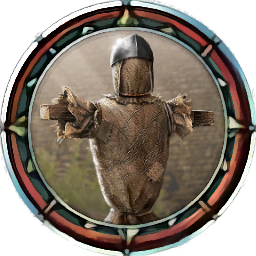
\includegraphics[width=70bp,height=70bp]{img/boss_token_example.png}
    \end{wrapfigure}

    Description of the Actor and token if possible. This description should be long enough so that the text goes below the token and wraps itself succesfully around it.

    More information should be presented, including tactical information. The token itself, obviously, is optional.
    
    %% IMPORTANT Implementation note: Remove the rpghline below if your description is not long enough to cover the token.
    \rpghline
    \stats[ % This 'stats' command will autocomplete the modifier for you
        % Correspondance with my rules : STR is MIG, DEX is DEX, CON is CON, INT is INT, WIS is WIT, CHA is RES
        STR = \stat{12}, 
        DEX = \stat{7},
        CON = \stat{10},
        INT = \stat{10},
        WIS = \stat{10},
        CHA = \stat{10},
    ]
    \rpghline

    % If you want to use commas in these sections, enclose the
    % description in braces.
    % I'm so sorry.

    \basics[
    armorclass = 3,
    hitpoints  = 42, %hitpoints  = \rpgdice{3d8 + 3},
    %speed      = 10,
    focus      = 5,
    defenses   = {Deflection 0, Reflex 0, Fortitude 0, Will 0}
    ]
    \rpghline%

    \details[%
    %% IMPORTANT: Many of those are optional and will default to empty if not specified.
    skills = {Athletics 3, Kosmics 1},
    accuracies = {Melee 6, Ranged 6},
    % languages = {Common Lisp, Erlang},
    % damageimmunities={Cosmic},
    % savingthrows=,
    % conditionimmunities={Charmed},
    % damageresistances={Electricity},
    % damagevulnerabilities={Fire},
    % senses=---,
    % languages=---,
    challenge=Elite,
    ]
    \rpghline%
    \begin{rpg-monsteraction}[Combat Specificities]
        Does this Actor have Reach ? Do they have a size larger than 1\texttimes 1 ? Do they have a different speed than standard? This can be listed here, with any other specificities.
    \end{rpg-monsteraction}

    \rpgmonstersection{Abilities and Actions}

    \begin{rpg-monsteraction}[Action Name]
        List any relevant Ability or Action. Including usable objects and any kind of special action.
    \end{rpg-monsteraction}

    \begin{rpg-monsteraction}[Combat Action Example]
        \textit{Accuracy vs Defense.} Effect.
    \end{rpg-monsteraction}


    \rpgmonstersection{Passive Abilities}

    \begin{rpg-monsteraction}[Trait]
    Any relevant Trait or Passive Ability. In particular, all Resistances and Vulnerabilities to Damage and Conditions should be listed here.
    \end{rpg-monsteraction}

    \begin{rpg-monsteraction}[Senses]
    Any relevant Sense or Language beyond what is commonly expected can be also listed here.
    \end{rpg-monsteraction}

    
    \rpgmonstersection{Notes}
    Optional. Any relevant note, such as the knowledge possessed by the Actor, roleplaying notes, advice about its intended combat behavior, maybe notes about possible variants of the Actor.

\end{monsterboxbg}


This Bestiary section will contain many standardized examples of Actors, ready for re-use.

Right above, I also present a template of "stat block", ready for modification and re-use: just look into the source code of the manuscript and see the implementation notes in the comments, or simply use it as a stylistic inspiration.

\begin{rpg-examplebox}
    Guidelines for the creation from scratch of custom Actors, as well as general balancing, are undissociable from general design considerations. As such, they are not presented here, but in section \ref{bestiary} instead. This part will instead contain only a catalog, and comments on the specific philosophy behind the design of the examples themselves, not of all Actors in general.
\end{rpg-examplebox}

The design considerations presented below also mean that Actors have, for instance, lower base damage and HP than would be the same for the players. As such, an easy way to scale these templates up when the players level up, so as to still match the guidelines, is to give them the equivalent of Tier 2 or Tier 3 equipment (or giving them objects that provide a similar boost in Aptitudes, Defenses and Damage).

\paragraph{Clarifications}

\begin{itemize}
    \item Although they are not written on the stat block, all Actors presented here also have access to all standard Actions, (such as Concentrate or Assist) unless specified otherwise.
    \item In the "Abilities and Actions" section, everything with the words "Standard Attack" or "Action" in the title is assumed to be a regular Action (meaning it does not cost Focus) and everything else is assumed to be an Ability (which costs Focus), unless specified otherwise.
    \item Each Ability or Action will mention in italics the Aptitude it uses, and if applicable, which Defense of the target to use as Difficulty ("vs"\footnote{If there is no "vs" (versus), then the Difficulty is 0. This is usually made up for by having weaker effects or asking for another roll in the description of the Ability.}), or even the formula of a roll that must be passed to trigger it. If there is instead written "\textit{Always succeeds}", it means the effects as written in the description will always trigger without needing a roll.
\end{itemize}



% Open with a new page
\newpage
\subsection{Examples of Actors}


\begin{monsterboxbg}{Zombie}

    A swarming enemy. Not so harmless in large groups.
    
    \rpghline
    \stats[
        STR = \stat{12}, 
        DEX = \stat{12},
        CON = \stat{8},
        INT = \stat{6},
        WIS = \stat{8},
        CHA = \stat{10},
    ]
    \rpghline

    \basics[
    armorclass = 0,
    hitpoints  = 12,
    focus      = 1,
    defenses   = {Deflection 1, Reflex 1, Fortitude 0, Will -2}
    ]
    \rpghline

    \details[%
    accuracies = {Melee 2, Ranged -2},
    challenge = Weak,
    ]
    \rpghline%
    \begin{rpg-monsteraction}[Combat Specificities]
        Abomination.
    \end{rpg-monsteraction}

    
    \rpgmonstersection{Abilities and Actions}

    \begin{rpg-monsteraction}[Standard Attack]
        \textit{Melee vs Deflection.} 2+1 damage.
    \end{rpg-monsteraction}

    \begin{rpg-monsteraction}[Ensnare]
        \textit{Melee vs Fortitude.} The target is Grappled. You can no longer act.
    \end{rpg-monsteraction}


\end{monsterboxbg}



\begin{monsterboxbg}{Warrior}

    A reliable sort, good at holding the line.
    
    \rpghline
    \stats[
        STR = \stat{14}, 
        DEX = \stat{14},
        CON = \stat{13},
        INT = \stat{8},
        WIS = \stat{8},
        CHA = \stat{10},
    ]
    \rpghline

    \basics[
    armorclass = 3,
    hitpoints  = 19,
    focus      = 3,
    defenses   = {Deflection 2+2, Reflex 2, Fortitude 3, Will -1}
    ]
    \rpghline

    \details[%
    skills = {Athletics 1},
    accuracies = {Melee 4, Ranged -2},
    ]
    \rpghline%

    
    \rpgmonstersection{Abilities and Actions}

    \begin{rpg-monsteraction}[Standard Attack]
        \textit{Accuracy vs Defense.} Shortsword and shield. 3+2 damage.
    \end{rpg-monsteraction}

    \begin{rpg-monsteraction}[Ever Vigilant]
    \end{rpg-monsteraction}

    \begin{rpg-monsteraction}[Stalwart]
    \end{rpg-monsteraction}

\end{monsterboxbg}




\begin{monsterboxbg}{Marskman}

    Lethal at range, can inflict heavy damage if allowed to set up in position.
    
    \rpghline
    \stats[
        STR = \stat{12}, 
        DEX = \stat{10},
        CON = \stat{12},
        INT = \stat{8},
        WIS = \stat{15},
        CHA = \stat{10},
    ]
    \rpghline

    \basics[
    armorclass = 1,
    hitpoints  = 18,
    focus      = 5,
    defenses   = {Deflection 2, Reflex 2, Fortitude 2, Will -1}
    ]
    \rpghline

    \details[%
    skills = {Discretion 2},
    accuracies = {Melee 0, Ranged 5},
    ]
    \rpghline%
    
    \rpgmonstersection{Abilities and Actions}

    \begin{rpg-monsteraction}[Standard Attack]
        \textit{Ranged vs Deflection.} Light musket. 6+1 damage, ignore 2 Armor, once per turn.
    \end{rpg-monsteraction}

    \begin{rpg-monsteraction}[Pin Down]
    \end{rpg-monsteraction}

    \rpgmonstersection{Passive Abilities}

    \begin{rpg-monsteraction}[Zeroing In]
        If you did not move on your previous turn, gain +1 to Accuracy.
    \end{rpg-monsteraction}

    \rpgmonstersection{Passive Abilities}

    A common variant will instead wield a Standard ranged weapon such as a crossbow.

\end{monsterboxbg}
            





\begin{monsterboxbg}{Daemon}

    The world is dark and full of terrors.
    
    \rpghline
    \stats[
        STR = \stat{14}, 
        DEX = \stat{16},
        CON = \stat{10},
        INT = \stat{14},
        WIS = \stat{10},
        CHA = \stat{12},
    ]
    \rpghline

    \basics[
    armorclass = 0,
    hitpoints  = 23,
    focus      = 5,
    defenses   = {Deflection 4, Reflex 4, Fortitude 4, Will 3}
    ]
    \rpghline

    \details[%
    skills = {Athletics 2},
    accuracies = {Melee 6, Ranged 0},
    ]
    \rpghline%
    \begin{rpg-monsteraction}[Combat Specificities]
        Abomination.
    \end{rpg-monsteraction}

    
    \rpgmonstersection{Abilities and Actions}

    \begin{rpg-monsteraction}[Standard Attack]
        \textit{Melee vs Deflection.} Claws. Deals 4+2 damage.
    \end{rpg-monsteraction}

    \begin{rpg-monsteraction}[Draining Touch]
        \textit{Melee vs Deflection.} Drain 6 HP.
    \end{rpg-monsteraction}

    \begin{rpg-monsteraction}[Intimidate]
        \textit{Always succeeds.} Target must pass [Will-6], or you inflict them with the "Intimidated" Condition (-3 to all Accuracies when attacking the caster)
    \end{rpg-monsteraction}

    \rpgmonstersection{Passive Abilities}

    \begin{rpg-monsteraction}[Darkvision]
    \end{rpg-monsteraction}


\end{monsterboxbg}




\begin{monsterboxbg}{Spellcaster}

    A polyvalent foe armed with a variety of Spells for all purposes, can become quite a headache if not dealth with quickly. Fortunately, not very resilient.
    
    \rpghline
    \stats[
        STR = \stat{10}, 
        DEX = \stat{8},
        CON = \stat{10},
        INT = \stat{14},
        WIS = \stat{14},
        CHA = \stat{12},
    ]
    \rpghline

    \basics[
    armorclass = 0,
    hitpoints  = 18,
    focus      = 6,
    defenses   = {Deflection 1, Reflex 1, Fortitude 0, Will 3}
    ]
    \rpghline

    \details[%
    skills = {Kosmics 2, Lore 2},
    accuracies = {Melee -2, Ranged 4},
    ]
    \rpghline%
    
    \rpgmonstersection{Abilities and Actions}

    \begin{rpg-monsteraction}[Standard Attack]
        \textit{Ranged vs Deflection.} Pistol. 4 damage, ignore 1 Armor.
    \end{rpg-monsteraction}

    \begin{rpg-monsteraction}[Frostbite]
        \textit{Ranged vs Fortitude.} 5 frost damage, and target loses 1 AP next turn.
    \end{rpg-monsteraction}

    
    \begin{rpg-monsteraction}[Toughen]
        \textit{Ranged.} Target gains +3 Deflection for the next turn only.
    \end{rpg-monsteraction}

    
    \begin{rpg-monsteraction}[Wand of Atrophy]
        \textit{Ranged vs Will.} 3 uses, does not cost Focus. Inflict the Ruptured Condition (+2 to all incoming damage).
    \end{rpg-monsteraction}

    
    \begin{rpg-monsteraction}[Reality Fault]
        \textit{Always succeeds.} Place a glyph on a distant tile. At the beginning of your next turn, it explodes, dealing 8 explosive damage on its tile and all adjacent tiles.
    \end{rpg-monsteraction}
    
    \begin{rpg-monsteraction}[Summon Sprites]
        \textit{Ranged.} Spawn two Sprites (Generic Enemy but with 4 HP only). Once per turn maximum.
    \end{rpg-monsteraction}


\end{monsterboxbg}
	





\newpage
\subsection{Challenging Enemies}




\begin{monsterboxbg}{Leader}

    Very adept at controlling the field of battle. Can become deadly when commanding a squad.
    
    \rpghline
    \stats[
        STR = \stat{15}, 
        DEX = \stat{12},
        CON = \stat{13},
        INT = \stat{12},
        WIS = \stat{8},
        CHA = \stat{14},
    ]
    \rpghline

    \basics[
    armorclass = 2,
    hitpoints  = 24,
    focus      = 6,
    defenses   = {Deflection 3, Reflex 3, Fortitude 3, Will 3}
    ]
    \rpghline

    \details[%
    skills = {Athletics 2, Psychology 2},
    accuracies = {Melee 2, Ranged -2},
    challenge = Veteran,
    ]
    \rpghline%
    
    \rpgmonstersection{Abilities and Actions}

    \begin{rpg-monsteraction}[Standard Attack]
        \textit{Melee vs Deflection.} Greatsword. 5+2 damage, ignore 2 Armor, once per turn.
    \end{rpg-monsteraction}

    \begin{rpg-monsteraction}[Into The Fray]
    \end{rpg-monsteraction}

    \begin{rpg-monsteraction}[Brute]
        \textit{Melee vs Fortitude.} Inflict Prone for the next turn only. On Graze, instead inflict Distracted (-2 to best Accuracy) for the same duration.
    \end{rpg-monsteraction}

    \begin{rpg-monsteraction}[Assault Order]
        \textit{Always succeeds.} Pick an enemy Actor. They get +2 to all incoming damage until the beginning of your next turn. Can stack up to +3.
    \end{rpg-monsteraction}

    \begin{rpg-monsteraction}[Walk It Off]
        \textit{Always succeeds.} Pick a friendly Actor. All hostile Conditions they suffer from are shortened by 1 turn (cannot shorten a Condition that has only 1 turn remaining).
    \end{rpg-monsteraction}

    \begin{rpg-monsteraction}[Sixth Sense]
    \end{rpg-monsteraction}

    \begin{rpg-monsteraction}[Second Wind]
    \end{rpg-monsteraction}

    \rpgmonstersection{Passive Abilities}

    \begin{rpg-monsteraction}[Thick of the Fight]
        All allies within 2 tiles of your position gain +1 to all Accuracies. You gain +1 to all Accuracies (up to +4) per such ally.
    \end{rpg-monsteraction}

\end{monsterboxbg}



\begin{monsterboxbg}{Hulking Monstrosity}

    The gloves are off. Face off against this enormous affront to Nature.
    
    \rpghline
    \stats[
        STR = \stat{20}, 
        DEX = \stat{14},
        CON = \stat{18},
        INT = \stat{10},
        WIS = \stat{10},
        CHA = \stat{12},
    ]
    \rpghline

    \basics[
    armorclass = 1,
    hitpoints  = 64,
    focus      = 5,
    defenses   = {Deflection 3, Reflex 3, Fortitude 9, Will 1}
    ]
    \rpghline

    \details[%
    skills = {Athletics 2},
    accuracies = {Melee 4, Ranged 0},
    challenge = Elite,
    ]
    \rpghline%
    \begin{rpg-monsteraction}[Combat Specificities]
        Large creature ($2 \times 2$ tiles). Abomination.
    \end{rpg-monsteraction}

    
    \rpgmonstersection{Abilities and Actions}

    \begin{rpg-monsteraction}[Standard Attack]
        \textit{Melee vs Deflection.} 3+5 damage, hits 2 adjacent tiles.
    \end{rpg-monsteraction}

    \begin{rpg-monsteraction}[Grab and Smash]
        \textit{MIG vs Reflex.} The target is Grappled by you. After 2 turns, if the Grapple was not broken, slam them to the ground for 10 damage.
    \end{rpg-monsteraction}

    \begin{rpg-monsteraction}[Clear Out]
    \end{rpg-monsteraction}

    \begin{rpg-monsteraction}[Hobbling Strike]
    \end{rpg-monsteraction}

    \rpgmonstersection{Passive Abilities}

    \begin{rpg-monsteraction}[Stalwart]
    \end{rpg-monsteraction}

    \begin{rpg-monsteraction}[Disgustingly Resilient]
        Regenerate 4 HP per turn.
    \end{rpg-monsteraction}


\end{monsterboxbg}



\begin{monsterboxbg}{Magister}

    Bear witness to the true power of Magic. A deadly foe, that can wield any kind of Spell imaginable to inflict any effect desired.
    
    \rpghline
    \stats[
        STR = \stat{12}, 
        DEX = \stat{14},
        CON = \stat{16},
        INT = \stat{20},
        WIS = \stat{16},
        CHA = \stat{16},
    ]
    \rpghline

    \basics[
    armorclass = 1,
    hitpoints  = 70,
    focus      = 12,
    defenses   = {Deflection 5, Reflex 5, Fortitude 6, Will 8}
    ]
    \rpghline

    \details[%
    skills = {Crafting 2, Kosmics 5, Lore 2},
    challenge = Elite,
    accuracies = {Melee 4, Ranged 6},
    ]
    \rpghline%
    
    \rpgmonstersection{Abilities and Actions}

    \begin{rpg-monsteraction}[Standard Attack]
        \textit{Ranged vs Deflection.} Pistol with enchanted bullets. Deal 4+1 magical damage.
    \end{rpg-monsteraction}

    \begin{rpg-monsteraction}[Knowledge Unending]
        Cast a Spell. \textit{See the Notes section!}
    \end{rpg-monsteraction}

    \begin{rpg-monsteraction}[Nightmare]
        \textit{Always succeeds.} Pick an Actor. Once per turn, perform opposed RES rolls, until the Actor is killed or you are interrupted. You cannot move in the process (this is a Channeling). Everytime the target wins, you deal them 3 psychic damage. Everytime they lose, move one step further on: (1) Inflict Sleeping, cannot be woken up with a simple Assist. (2) Take 10 psychic damage. -4 to Intelligence, Wits and Resolve until rest. (3) Instantly drop to 0 HP.
    \end{rpg-monsteraction}


    \rpgmonstersection{Passive Abilities}

    \begin{rpg-monsteraction}[Mind Over Matter]
        +1 Accuracy when casting Spells. All negative mental Conditions recieved are downgraded (ie. Dominated becomes Charmed).
    \end{rpg-monsteraction}

    
    \rpgmonstersection{Notes}

    In the context of the "Knowledge Unending" Ability, to determine which Spells are known to a given Magister, you can draw from anywhere in this manuscript, depending on roleplaying context of course to inform your picks. For instance, it can be assumed they know all the Spellcaster archetype does, but feel free to draw Spells from any example given in the manuscript. Keep them reasonably balanced, for instance by downgrading Boss spells if you pick them.
    
    Furthermore, the second example included here (Nightmare) is an example of how Magisters have access to very powerful Spells beyond the reach of the players (at least in the beginning...), but feel free to design your own broken Abilities.

\end{monsterboxbg}









\begin{monsterboxbg}{Eidolon of the Dreamers}

    The cosmos would be a better place, if certain things were to never see the light again.
    
    \rpghline
    \stats[
        STR = \stat{16}, 
        DEX = \stat{14},
        CON = \stat{22},
        INT = \stat{10},
        WIS = \stat{10},
        CHA = \stat{12},
    ]
    \rpghline

    \basics[
    armorclass = 0,
    hitpoints  = 200,
    focus      = 12,
    defenses   = {Deflection 1, Reflex 1, Fortitude 9, Will 2}
    ]
    \rpghline

    \details[%
    skills = {Athletics 2},
    accuracies = {Melee 4, Ranged 0},
    challenge = Boss,
    ]
    \rpghline%
    \begin{rpg-monsteraction}[Combat Specificities]
        Large creature ($2 \times 2$ tiles). Abomination.
    \end{rpg-monsteraction}

    
    \rpgmonstersection{Abilities and Actions}

    \begin{rpg-monsteraction}[Standard Melee Attack]
        \textit{Melee vs Deflection.} Smash, dealing 7+2 damage on two tiles adjacent to each other.
    \end{rpg-monsteraction}

    \begin{rpg-monsteraction}[Standard Ranged Attack]
        \textit{Ranged vs Deflection.} Scorpio bolt. 5+2 damage.
    \end{rpg-monsteraction}

    \begin{rpg-monsteraction}[Clear Out]
    \end{rpg-monsteraction}

    \begin{rpg-monsteraction}[Neural Network]
        \textit{Always succeeds.} All visible Abominations, including yourself, permanently gain +1 to all Aptitudes. Cumulative up to +6. Once per turn only.
    \end{rpg-monsteraction}

    \begin{rpg-monsteraction}[Unmake Them]
        \textit{Melee vs Reflex.} Grapple a target. Slam it to the ground at the beginning your next turn, dealing 8 damage.
    \end{rpg-monsteraction}

    \rpgmonstersection{Passive Abilities}

    \begin{rpg-monsteraction}[Presence]
        Immune to Knockback and Dominated.
    \end{rpg-monsteraction}

    \begin{rpg-monsteraction}[Boss]
        Gains 3 AP per turn instead of 2. Stuns instead reduce AP by 2.
    \end{rpg-monsteraction}

    \begin{rpg-monsteraction}[Tactical Retreat]
        Upon losing 30 total HP, hide in the darkness and come down upon hearing noise. Repeat until defeated.
    \end{rpg-monsteraction}

\end{monsterboxbg}








\begin{monsterboxbg}{Arch Lector}

    The Magister to rule them all.
    
    \rpghline
    \stats[
        STR = \stat{14}, 
        DEX = \stat{16},
        CON = \stat{22},
        INT = \stat{30},
        WIS = \stat{22},
        CHA = \stat{24},
    ]
    \rpghline

    \basics[
    armorclass = 2,
    hitpoints  = 220,
    focus      = 15,
    defenses   = {Deflection 10, Reflex 10, Fortitude 13, Will 17}
    ]
    \rpghline

    \details[%
    skills = {Kosmics 10, Psychology 2, Lore 5, Athletics 3},
    accuracies = {Melee 6, Ranged 12},
    challenge = Nightmare Boss,
    ]
    \rpghline%
    \begin{rpg-monsteraction}[Combat Specificities]
        Human-ish.
    \end{rpg-monsteraction}

    
    \rpgmonstersection{Abilities and Actions}

    \begin{rpg-monsteraction}[Standard Attack]
        \textit{Melee vs Deflection.} Shortsword. Deals 7+2 damage.
    \end{rpg-monsteraction}

    \begin{rpg-monsteraction}[Lunge]
        \textit{Melee.} Move in a straight line over 4 squares. All Actors in your path take 7+2 damage (cannot avoid it) and must pass [Fortitude-6] or be Knocked Down for 1 turn only.
    \end{rpg-monsteraction}

    \begin{rpg-monsteraction}[Fate of the Sworn]
        \textit{Always succeeds.} Resurrect an Actor, who was friendly to you, with half its Hit Points.
    \end{rpg-monsteraction}

    \begin{rpg-monsteraction}[Vainquish]
        \textit{Ranged vs Reflex.} Hurl a lightning bolt at a distant enemy, dealing 8+2 lightning damage and inflicting -1 to all Defenses for 2 turns only (can stack).
    \end{rpg-monsteraction}

    \begin{rpg-monsteraction}[Blink]
        \textit{Always succeeds.} Teleport away. All enemies adjacent to your initial position must pass [Fortitude-6] or be Blinded for 1 turn only.
    \end{rpg-monsteraction}

    \begin{rpg-monsteraction}[Death From Above]
        \textit{Always succeeds.} Pull a golden bow and mark an area of diameter 4. Every Actor in the area at the beginning of your next turn takes 15 damage, and you inflict them with Burning (2 damage per turn). Cannot be avoided.
    \end{rpg-monsteraction}

    \begin{rpg-monsteraction}[Deny the Witch]
        \textit{Ranged vs Will.} Target is Silenced for their next turn (cannot use Abilities or Gadgets).
    \end{rpg-monsteraction}

    \begin{rpg-monsteraction}[Dominate]
        \textit{Ranged.} Target must pass [Will-8] (Grazes count) or be Dominated for their next turn.
    \end{rpg-monsteraction}

    \rpgmonstersection{Passive Abilities}

    \begin{rpg-monsteraction}[Lightning Reflexes]
        Like Ever Vigilant, except the AP granted can be used to cast Abilities.
    \end{rpg-monsteraction}
        
    \begin{rpg-monsteraction}[Boss]
        Gains 3 AP per turn instead of 2. Stuns instead reduce AP by 2.
    \end{rpg-monsteraction}

    \begin{rpg-monsteraction}[Unbreakable Spirit]
        Recover 1 Focus per turn. All negative mental Conditions recieved are downgraded (ie. Dominated becomes Charmed).
    \end{rpg-monsteraction}

    \rpgmonstersection{Notes}
    This Boss has particulary high Defense values (and Accuracies to a lesser degree). As such, it is meant to be fought by players which have been boosted: they should regain some Heroism each turn, and use it to overcome this Boss.

    Note that the Abilities of the boss themselves are powerful, but not insanely so. The difficulty really comes from the modifiers.

\end{monsterboxbg}



\section{Examples of Abilities}

\label{examples}

This section presents example of Spells (in Table \ref{spells_example_table}), but also of Gadgets (in Table \ref{gadgets_example_table}) and Traits (in Table \ref{traits_example_table}). 


\begin{rpg-examplebox}


Those examples are here to be used as an inspiration when designing your own! As mentioned before, you can also \textbf{draw on the custom Abilities in the Bestiary above} for inspiration.
\end{rpg-examplebox}


In those examples, to determine the duration of Conditions an INT of 3 and a target RES of 1 is assumed.

Some examples of uses that are different from a simple damage value or applied modifiers are presented, such as "Douse in Oil". We also present examples of different Objects created by achieving certain results when Crafting: for example, a a "Superior Ice Bomb" is obtained by a Critical Success when crafting an "Ice Bomb".

Those examples are useful to understand the construction and balancing of a Spell, or a custom Ability in general. For instance, consider "Unlife": in terms of expected effect, this is roughly the equivalent of being able to inflict 3 damage \texttimes 3 turns \texttimes 2 actions per turn \texttimes 0.5 from the hit probability, plus having a meatshield which will in effect prevent some HP damage to the PCs. This is slightly more powerful than other Abilities, but not much so, and is paid for by necessitating 6 Power Accents. As discussed before, always think in terms of \textbf{"how big of an impact does one use of this Ability have on the field of play"}.

\begin{table*}[h!tbp]
	\begin{center}
		\begin{tabular}{p{2.5cm}p{2cm}p{3.5cm}p{7.5cm}} \toprule
			
		    \textbf{Name} & \textbf{Sigil} & \textbf{Accents} & \textbf{Effect} \\ \midrule

		    Cone of Intense Frost & Frost & Spray, Power 3 & vs Fortitude. 7 Frost damage in a cone. \\[2mm] 
            Cone of Biting Frost & Frost & Spray, Power 3 & vs Fortitude. 5 Frost damage in a cone, and targets lose 1 AP next turn. \\[2mm] 

            System Shock & Lightning & Power 4 & vs Fortitude. On touch, inflicts Stunned. \\[2mm] 

            Trip & Force & Impact 2, Power 1 & vs Fortitude. Range of 10 tiles. Inflict Tripped (\times 0.5 Movement) for 3 turns, or move a small object. \\[2mm] 

            Apparitions & Summoning & Impact 2, Power 2, Duration & vs Will. Inflicts Distracted (-2 to all melee combat rolls). \\[2mm] 

            Douse in Oil & Telluric & Impact, Duration, Power 2 & vs Reflex. Douses in flammable oil for 3 turns.  \\[2mm] 

            Fire sword	& Fire	& Affect item, Power 1, Duration & For 3 attacks, your weapon deals 2 additional Fire damage. \\[2mm] 

            Frost Shell & Frost & Effect on self, Duration & Cancel the next 5 Fire damage. Then is Wet for 3 turns. \\[2mm] 

            Unlife  & Summoning & Power 6, Duration & On touch, turn a fresh corpse into a Standard Enemy (15 HP, 3 to all Aptitudes, 2 to all Defenses) for 3 turns, controlled by the caster. \\[2mm]

            Illusory Disguise & Illusion & Power 3, Effect on self, Duration & Disguise yourself as something specific. +5 to Discretion for rolls involving this disguise. Lasts 3 turns in combat, but a few minutes out of combat. \\[2mm] 

		    \bottomrule
		\end{tabular}
	\end{center}
	\caption{Examples of Spells}
  \label{spells_example_table}
\end{table*}



\begin{table*}[h!tbp]
	\begin{center}
		\begin{tabular}{p{4cm}p{12cm}} \toprule
			
		    \textbf{Name} & \textbf{Effect} \\ \midrule

		    Bodkin Arrow & Ignore 2 Armor. \\[2mm] 

            Invigorating Salts & On touch, heal 7+INT HP. \\[2mm] 

            Kinetic Petards & vs Fortitude. Area of Effect (1 square radius). Pushes targets by 1 square away, from the point of impact. They cannot Sidestep on their next turn. \\[2mm] 
          
            Hailpowder & Thrown at an ally. For the next 3 attacks against them, 5 damage is dealt to the attacker. \\[2mm] 
            
            Ice Bomb & Applies Ice on the ground (2 squares radius), for 3 turns. Anyone who moves on the ice must succeed in a flipped Reflex roll with a Difficulty of 5 or be knocked Prone for 3 turns. Ice will melt. \\[2mm] 
            Superior Ice Bomb &	All of Ice Grenade, plus everybody in the blast radius loses 1 AP. \\[2mm] 

            Inscribed Storm Bullet & Convert up to 5 damage into lightning (magic) damage. \\[2mm] 

            Sticky Grenade & vs Deflection. Inflicts 10 explosive damage on the next turn. [DEX-5] to halve the damage. \\[2mm] 

            Mindspin Wand & vs Will. One use. Inflict at random a Condition among: Charmed, Frightened, Enraged. Lasts 3 turns. \\[2mm] 

		    \bottomrule
		\end{tabular}
	\end{center}
	\caption{Examples of Gadgets}
  \label{gadgets_example_table}
\end{table*}

\begin{table*}[h!tbp]
	\begin{center}
		\begin{tabular}{p{4cm}p{12cm}} \toprule
			
		    \textbf{Name} & \textbf{Effect} \\ \midrule

		    Full-method Acting & +2 to Disguise, but can only wear Boot Dagger when disguised. \\[2mm] 

            Disfigured & When unmasked, -2 to Psychology, but +2 instead when intimidating. \\[2mm] 

		    \bottomrule
		\end{tabular}
	\end{center}
	\caption{Examples of Traits}
  \label{traits_example_table}
\end{table*}


%% Strategy layer/campaign
\chapter{Grandstrategy}

Those Grand Strategy, or "Grandstrategical" rules if you'll forgive this portmanteau, are \textbf{very optional}. Use them only if you wish to add a grand strategy component to your campaign, with geopolitics and military manoeuvers.

\label{strategy_rules}

The grand strategic map is divided into \textbf{provinces}. Depending on the scale of your campaign, I recommend that a province should cover an area with a diameter of roughly 80-100km in densely populated areas, a larger diameter in less populated ones, and a much larger diameter for the sea. Of course this can be scaled up or down. Each turn represents something like a few weeks, depending on the scale.

If you are using the same map as the ones used for your PC's travels, then instead I recommend that the provinces should be smaller and each turn represent only one week.

Players take their turns one after the other. In this instance, a "Player" designates a faction or more generally a side, not an individual Player Character: the PCs are one faction by themselves. The scenario designates which player goes first.

\begin{rpg-examplebox}
	As with the core rules, the Game Master may assign any modifier they wish to any roll, or change any rule, to account for specific circumstances.
\end{rpg-examplebox}


\section{Player turn}

A turn consists of two Phases: Economy and Action, taken in that order.

\begin{enumerate}
    \item \textbf{Economy Phase}: recruit Armies (and Agents), place Buildings, collect income, pay upkeep.
    \item \textbf{Action Phase}: Units movement and combat, and Agents can act.
    \item Pass to next player.
\end{enumerate}

Within a Phase, you can do the allowed actions in any order you wish: for example during the Action phase, you may use an Agent, then an Army, then another Agent, etc.


\section{Provinces}

Each controlled Province grants an income of 1G (Gold, representing resources in general) per turn at the beginning the Economy phase.

A Province is captured automatically when a Player's Units move inside it, unless troops from another Player are present: in this case, there is a battle (see later).


\subsection{Buildings}

\rpgart{t}{img/art/fort}

Each Province has 2 Building slots. During the Economy phase, you may pay 4G to build a Building in the first slot, or pay 6G to build in the second slot if the first slot is already occupied. The building is placed face down, and activated at the beginning of your next Economy phase.

Here are the standard Buildings:

\begin{itemize}
    \item \textbf{City}: Gives +2G per turn
    \item \textbf{Barracks}: allows Unit recruitment, and adds fortifications (+3 in a defensive battle)
\end{itemize}

A province with both a City and a Barracks will need to be sieged before being captured.

Relatedly, It should be noted that "Building" is actually a very general concept representing any kind of distinctive feature, as is explained in the Special Buildings section below.

\section{Armies}

An Army is a stack of Units, that can move and fight on the main map.

Armies have 2 move points per turn. Moving to an adjacent province usually costs 1 point\footnote{Army move speeds will need to be tweaked depending on how much time each turn represents, or the province sizes.}. Armies in friendly territory can move faster with an Agent action.


\subsection{Recruitment}

To recruit an Unit during the Recruitment phase, pick a Province with a Barracks. When recruited, the Unit is placed face down and will activate at the beginning of your next Economy phase. Each Barracks can recruit at most 2 Units per turn. Note that Units cannot be recruited in conquered territories until 3 turns after the conquest\footnote{Unless you are reconquering one of your core territories}.

You can either recruit generic Units at a cost of 1G each, or more costly Unique Units. Unique Units are created by the GM and will generally give a bonus if certain conditions are met. An example: "Heavy Cavalry, gives +1 in Late Phase unless the enemy has Pikes". Multiple Unique Units can be stacked in the same army, and their modifiers are cumulative.

Each regiment necessitates an upkeep of 1G per turn, during the Upkeep phase. 
Heroes require no upkeep. 

Fleets are required to cross naval provinces\footnote{In certain scenarios, Fleets may be abstracted by a maritime movement path between two provinces, but this is not the general case.}. Fleets are recruited with the same principle as land Units, except they cannot enter land provinces but may occupy port. The player simply declares that they wish to recruit a naval Unit instead of a Land unit. 


\paragraph{Battles}

When an Army encounters another Army belonging to an enemy player in the same province, they automatically initiate a Battle if possible. Note that each Army can initiate only one battle per turn, and as such cannot invade an occupied province if they already fought this turn, even if they have Movement left.

Each Battle consists of two rolls, with the usual "d20 + modifier" core rules; Those rolls are called respectively the Early and the Late roll\footnote{The Early phase represents manoeuvers, skirmishes and early contacts, while the Late phase represents the main engagement and pursuits}. Unique Units and Agents can apply a modifier to any of those rolls.

The roll is made by the attacker, and the modifier is equal to the difference in number of Units, plus the modifiers from Unique Units. Obviously, all of these are added positively for the attacker and negatively for the defender.

Whoever loses the first roll gets -2 for the second roll. After the Battle, each side loses 25\% of their Units per roll they lost and 5\% per roll they won rounded down. Each player chooses which of their units to remove). Here "Grazes" count as Failures, resulting in a symmetrical success table, for balance reasons.

An army that loses two rolls must retreat to their choice of an adjacent friendly province, and is destroyed if they cannot. In case of a draw, both Armies may stay in place and a new Battle is initiated next turn, or choose to retreat.

While any land battle, siege and naval battles can be resolved with the those rules, if you want to be a bit more involved there are rules for that in section \ref{operations}.


\subsection{Capturing a province} 

As mentioned before, Provinces are captured by moving an Army into them, but only if there are no defending Armies in it. This means that, for example, in case of a tie in a Battle you will not capture the province unless all defenders were destroyed.

When a province is conquered, the building in the second slot is destroyed.


\section{Setup}

When beginning the strategic scenario, the GM will decide on the initial placement of Armies, Buildings, Agents, etc. If the scenario does not specify it, each Player starts with no assets and 2G.

The Game lasts until the Victory Conditions specified by the GM are met.


\subsection{Special Buildings} 

As we discussed before, a "Building" is a very general concept, which is in fact closer to representing any "province feature" and may have its own rule.

For example, basic custom buildings may give different modifiers (mine, farm, temple, school, etc.) or represent the availability of special resources. But, for example, a movable "building" could represent a guerilla effort in another Player's province, or the vassalage of local nobles. Terrain features may also be represented; as explained in the other strategic rules, terrain can affect movement, combat and economy.

\section{Agents}

\label{agents}

Agents are special Actors, and this also includes Heroes (Player Characters and other important \textit{dramatis personae}). They are represented as Pawns on the campaign map.

Agents are (N)PC and have a character sheet, but in practice, they will be described based on their role. For instance, a "+5 Spy" is an Actor with +3 DEX and 2 Discretion\footnote{Note that acting on a strategic scale has an inherently higher Difficulty}.

The cost to recruit Agents depend on their quality (modifier for their role), and may be given by the scenario. Indeed, in the latter cases, most Heroes can be Agents.

Agents move twice as fast as Armies. Armies can not intercept Agents in the general case, but it is possible to make a roll for it if there is a siege or a significant event.

\subsection{Agent Actions}

Each turn, a player may describe and the GM adjudicates 1 action per Agent during the Action phase.

Here are some examples of such actions: 

\begin{itemize}
    \item Lead an Army, granting combat bonuses.
    \item Spying to reveal intel.
    \item Assassinate another agent.
    \item Stimulate the local economy.
\end{itemize}

I think those should be present in most games, but feel free to add some beyond that. 

The GM decides what rolls each Action entails. They are adjudicated with the usual core roll rules: 1d20 + Aptitude, Difficulty and relevant modifiers. In terms of impact on the game board, it should be roughly equivalent to a battle.

For the PC's actions, you can use this principle as well, but I recommend using Snapshots as seen below. This is a Role-Playing Game after all!


\subsection{Autonomous Agents}

If the GM decides, NPC Agents can have an will of their own. Each turn, such an Autonomous Agent each turn, picks Action to do depending on their chosen Agenda. Agendas can be influenced by other Actors (including the PC), learning from the consequences of past actions, etc.



\section{Snapshots}

We must not forget that this is a Tabletop Role-Playing Game! As such, all events in the grand strategy campaign such as Battles or Agent Actions can have Snapshots. Those are key moments and scenes, played with the classical RPG rules, that are part of the scenario and are in fact a way to "zoom" from strategic to a RPG scene.

For example, a battle could be played using the operational combat rules mentioned in another section, and some key moments such as an infiltration or a last stand can be played in the RPG scale. In this case, the diegetic outcome of the Snapshot should influence the final result.

Indeed, for Agent Actions, if the PC are involves they can and should play them directly with RPG rules, as part of the scenario\footnote{It is always the case for the "main quest", at the GM's discretion.}.

The goal of these grand strategy rules is to be an accelerator of gameplay and a story generator: as such, the parts that are interesting to the story will be played as an RPG, and the tedious parts can be abstracted away with those rules.


\subsection{Deepening the rules}

Finally, if you zoom in even at the strategic map level, consider the Operations as presented in section \ref{operations}. When playing at the grand strategy level, most of these are abstracted away in the Movement Points, Buildings, etc. but can be worth keeping in mind, Reputations in particular.


\section{Special rules}

Building upon this framework, the GM can add any manner of Special Rules to represent certain aspects of situations.


\subsection{Faction bonus}

Some players (factions) may get some inherent advantages (equivalent of Traits) to represent cultural specificities. Examples: improved Unique Units, reduced Upkeep in certain conditions, faster constructions, better fortifications, can relocate buildings, etc.

\subsection{Events}

The scenario may have planned certain special Events, that can trigger if certain conditions are met and affect the game board and player status in any possible way: for instance, switch control of provinces, give modifiers, place new Pawns, modify diplomatic relations, natural events, etc. This is also a general category for any modification the GM may wish to make to the state of play.

Events are conceptually linked to Agent Actions (the result of such an Action is an Event). They can affect the board in any way (ie. camouflaging an Army can be an Event) and may represent not only military actoins, but also political and diplomatic maneouvering.

\subsection{Diplomacy}

There are no specific rules for diplomacy between human players. Diplomacy with other Factions will likely be mediated by Agent Actions. However, in general, Diplomacy will also likely be handled by the plot itself. 

Alternatively, it is very possible use something like the Reputations framework, presented in section \ref{reputations} and expanded for strategical concerns in section \ref{relations}: so that each faction can accumulate Reputation with another faction. A quick example would be to let major factions improve their Reputation (then Influence) with a minor faction through spending resources for assistance (or coercion...). This would in turn impact their diplomatic reputation with other powers.

Also consider that factions, like autonomous NPCs, can have Agendas which define explicitly their objectives, priorities, and what they will try to negotiate for. Reputations and Agendas combined quantify each faction's willingness to respectively accept and propose certain deals with each other, and by extension their willingness to oppose each other or cooperate.

%% Lore
\chapter{Lore}

The \textit{Dreamshard} system was designed to be rather polyvalent, and can fit a variety of settings. That being said, it was built with its own custom setting in mind: a late medieval, low-fantasy world, which I shall present in this appendix.

\paragraph{In brief...}

In the recent past, the Dreamshard Isles have been shaken by unexplained magical phenomena. This, combined with an increase in finding of rare artifacts from the fabled Voskari mages, has attracted much outsider interest. More recently, the situation culminated with a volcanic eruption on Faris Island, which Magisters suspect might not be entirely natural... 

This is compounded by an already unstable geopolitical background with expansion efforts by the Atheryn Empire and other nations, while powerful Magisters vie for influence. The IDC, a branch of the Empire, is trying to expand in the Dreamshards and assert its influence, but other polities do as well. 

The players\footnote{Note that in terms of capabilities, the Player Characters as described by the rules are already a fair measure above a good chunk of the general population, especially when it comes to Magic.} are mandated by the governor of the Empire's portion of the Dreamshards, a man named Lucius Clarence, to investigate the situation. They secured a ride on a ship, and are headed for the city of Port-Darla, a major metropolis and headquarters of the IDC.

\textit{What will they find? And should it have remained in the shadows?}


\section{Map}

The known world consists of four major landmasses: first, the Dreamshard archipelago to the west, presented on Map \ref{map_1}. Second, the planet's largest continent, home to the Eastern Realms and located in the center of most world maps; it is partially presented in Map \ref{map_2}. Two other major continents exits: one to the east of the Eastern Realms (ironically), and one to the south.


\begin{figure*}[ht!]
    \centering
    \resizebox{0.85\textwidth}{!}{
        %\includesvg{img/map/map.svg}
        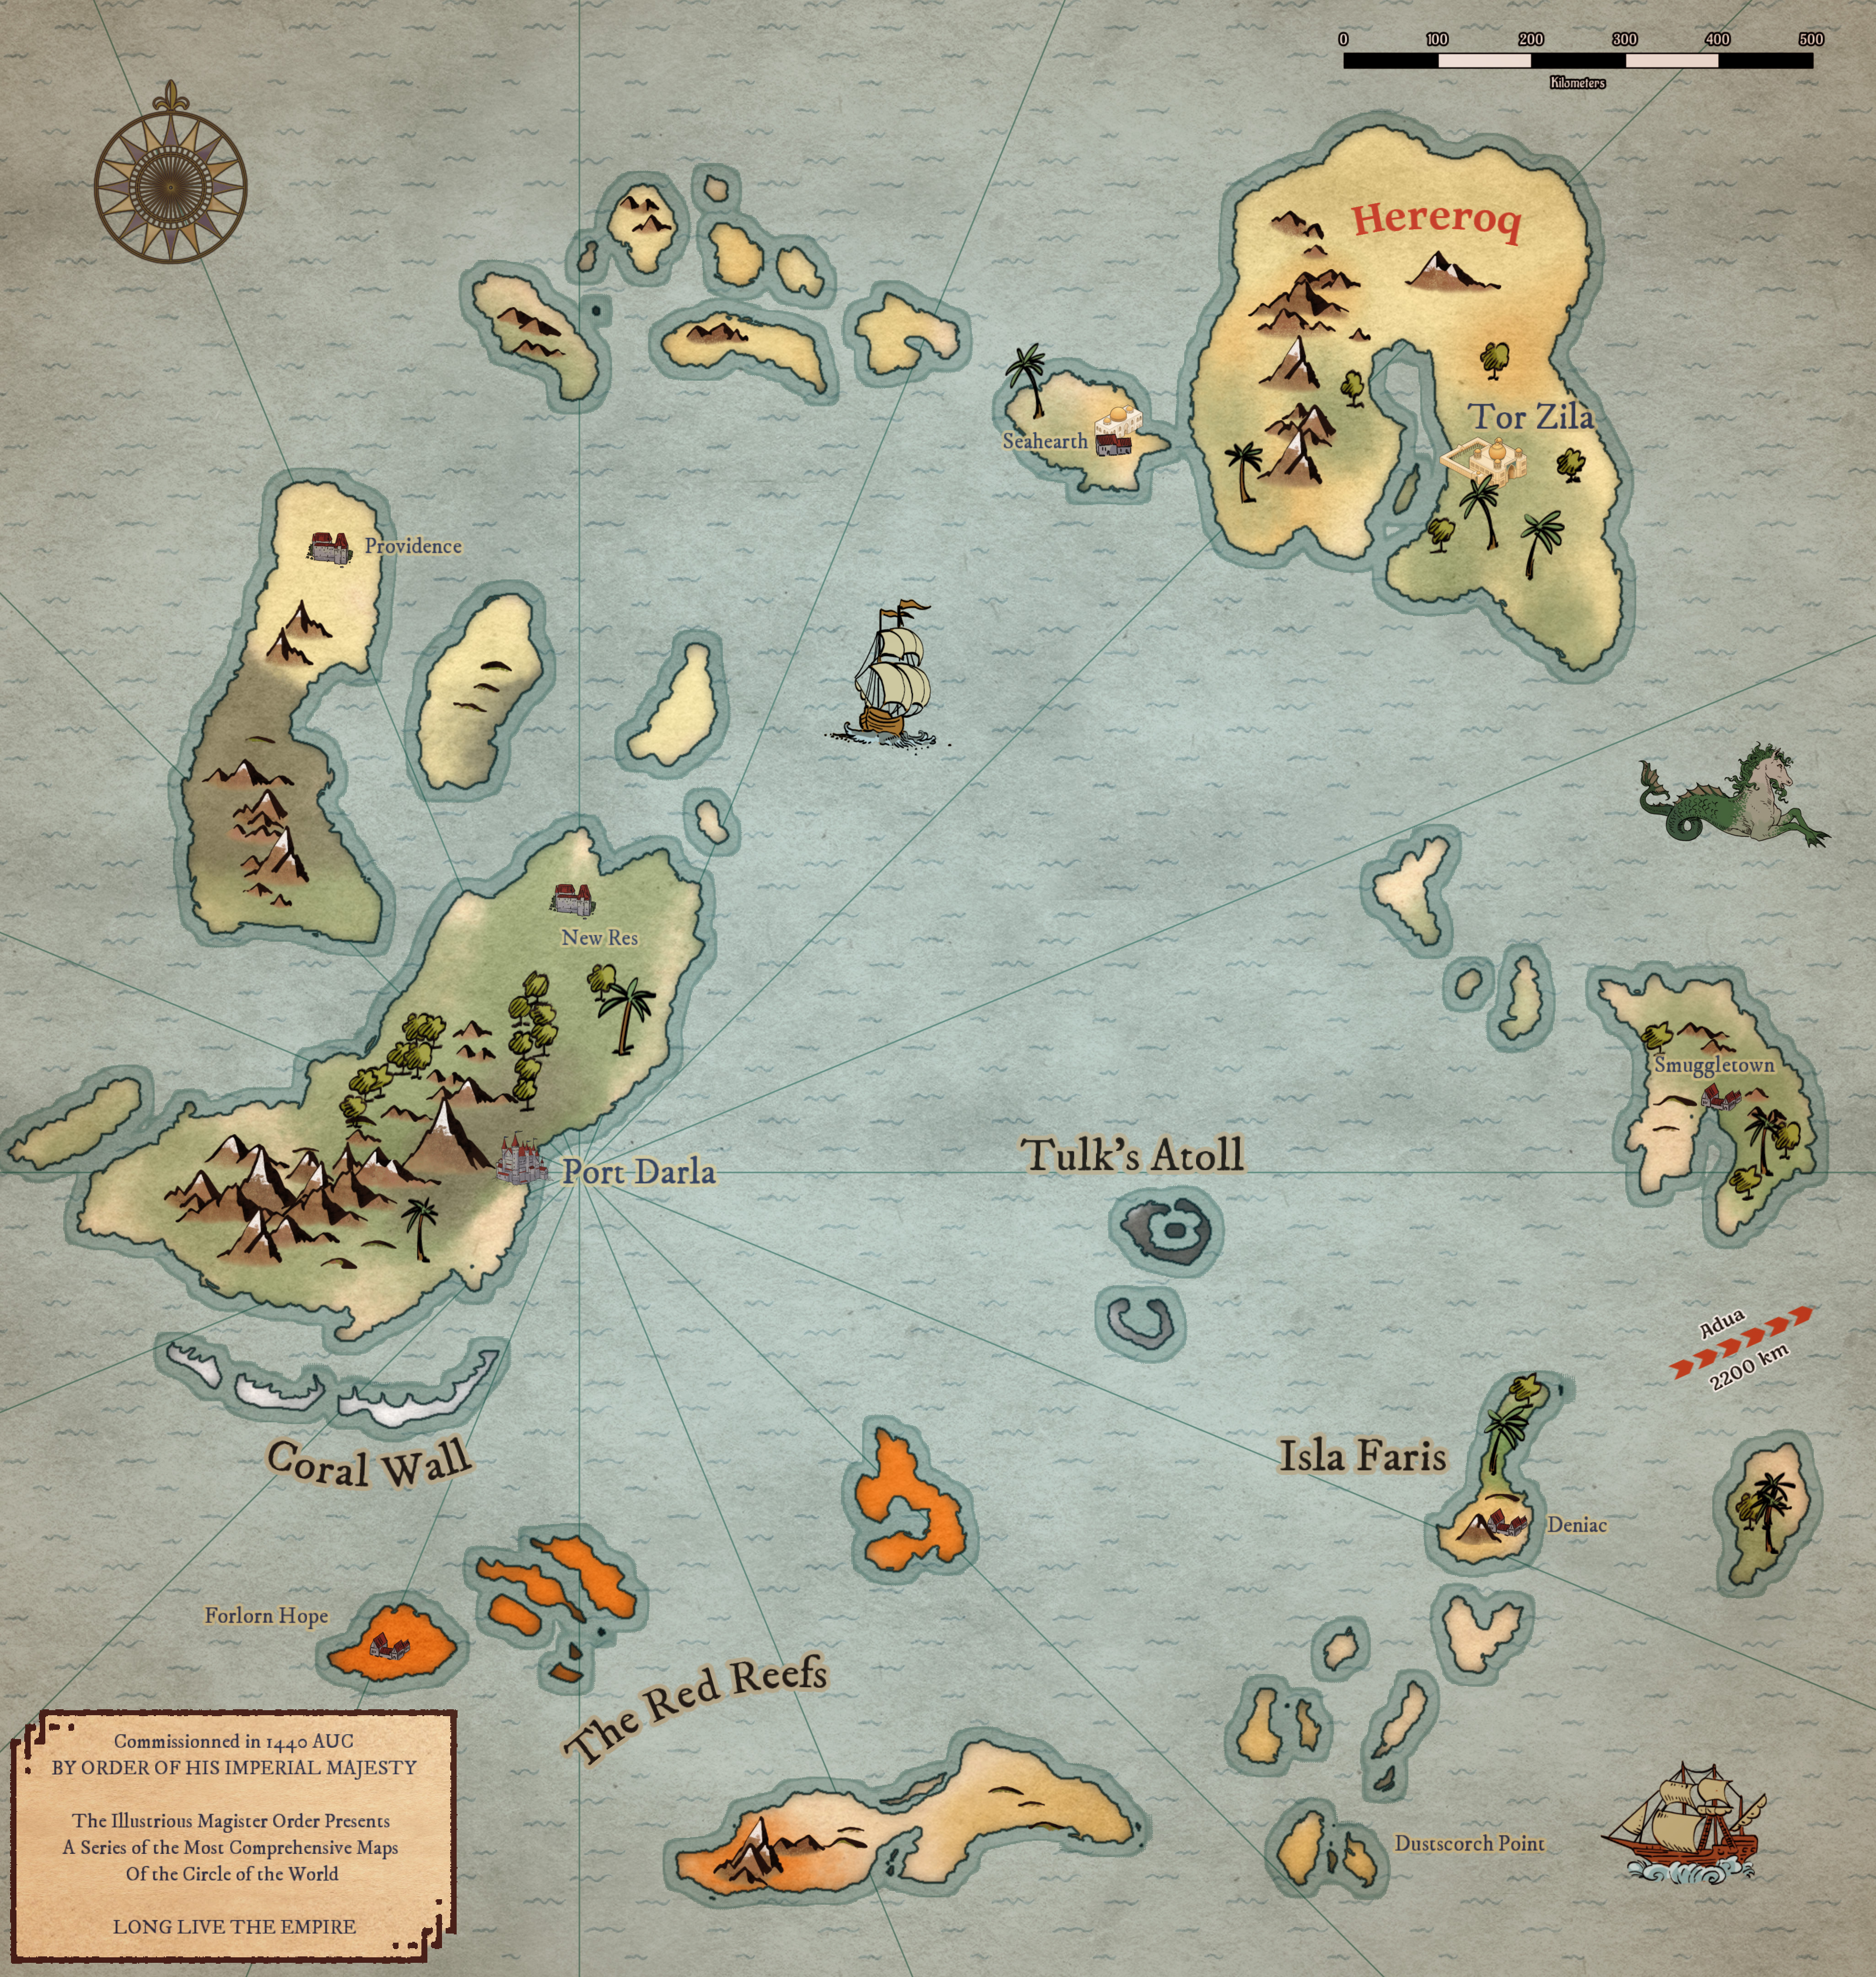
\includegraphics[angle=0,origin=c]{img/map_dreamshard.jpg}
    }
    \caption{Map of the Dreamshard Archipelago. Only major settlements are represented.}
    \label{map_1}
\end{figure*}


\begin{figure*}[ht!]
    \centering
    \resizebox{0.85\textwidth}{!}{
        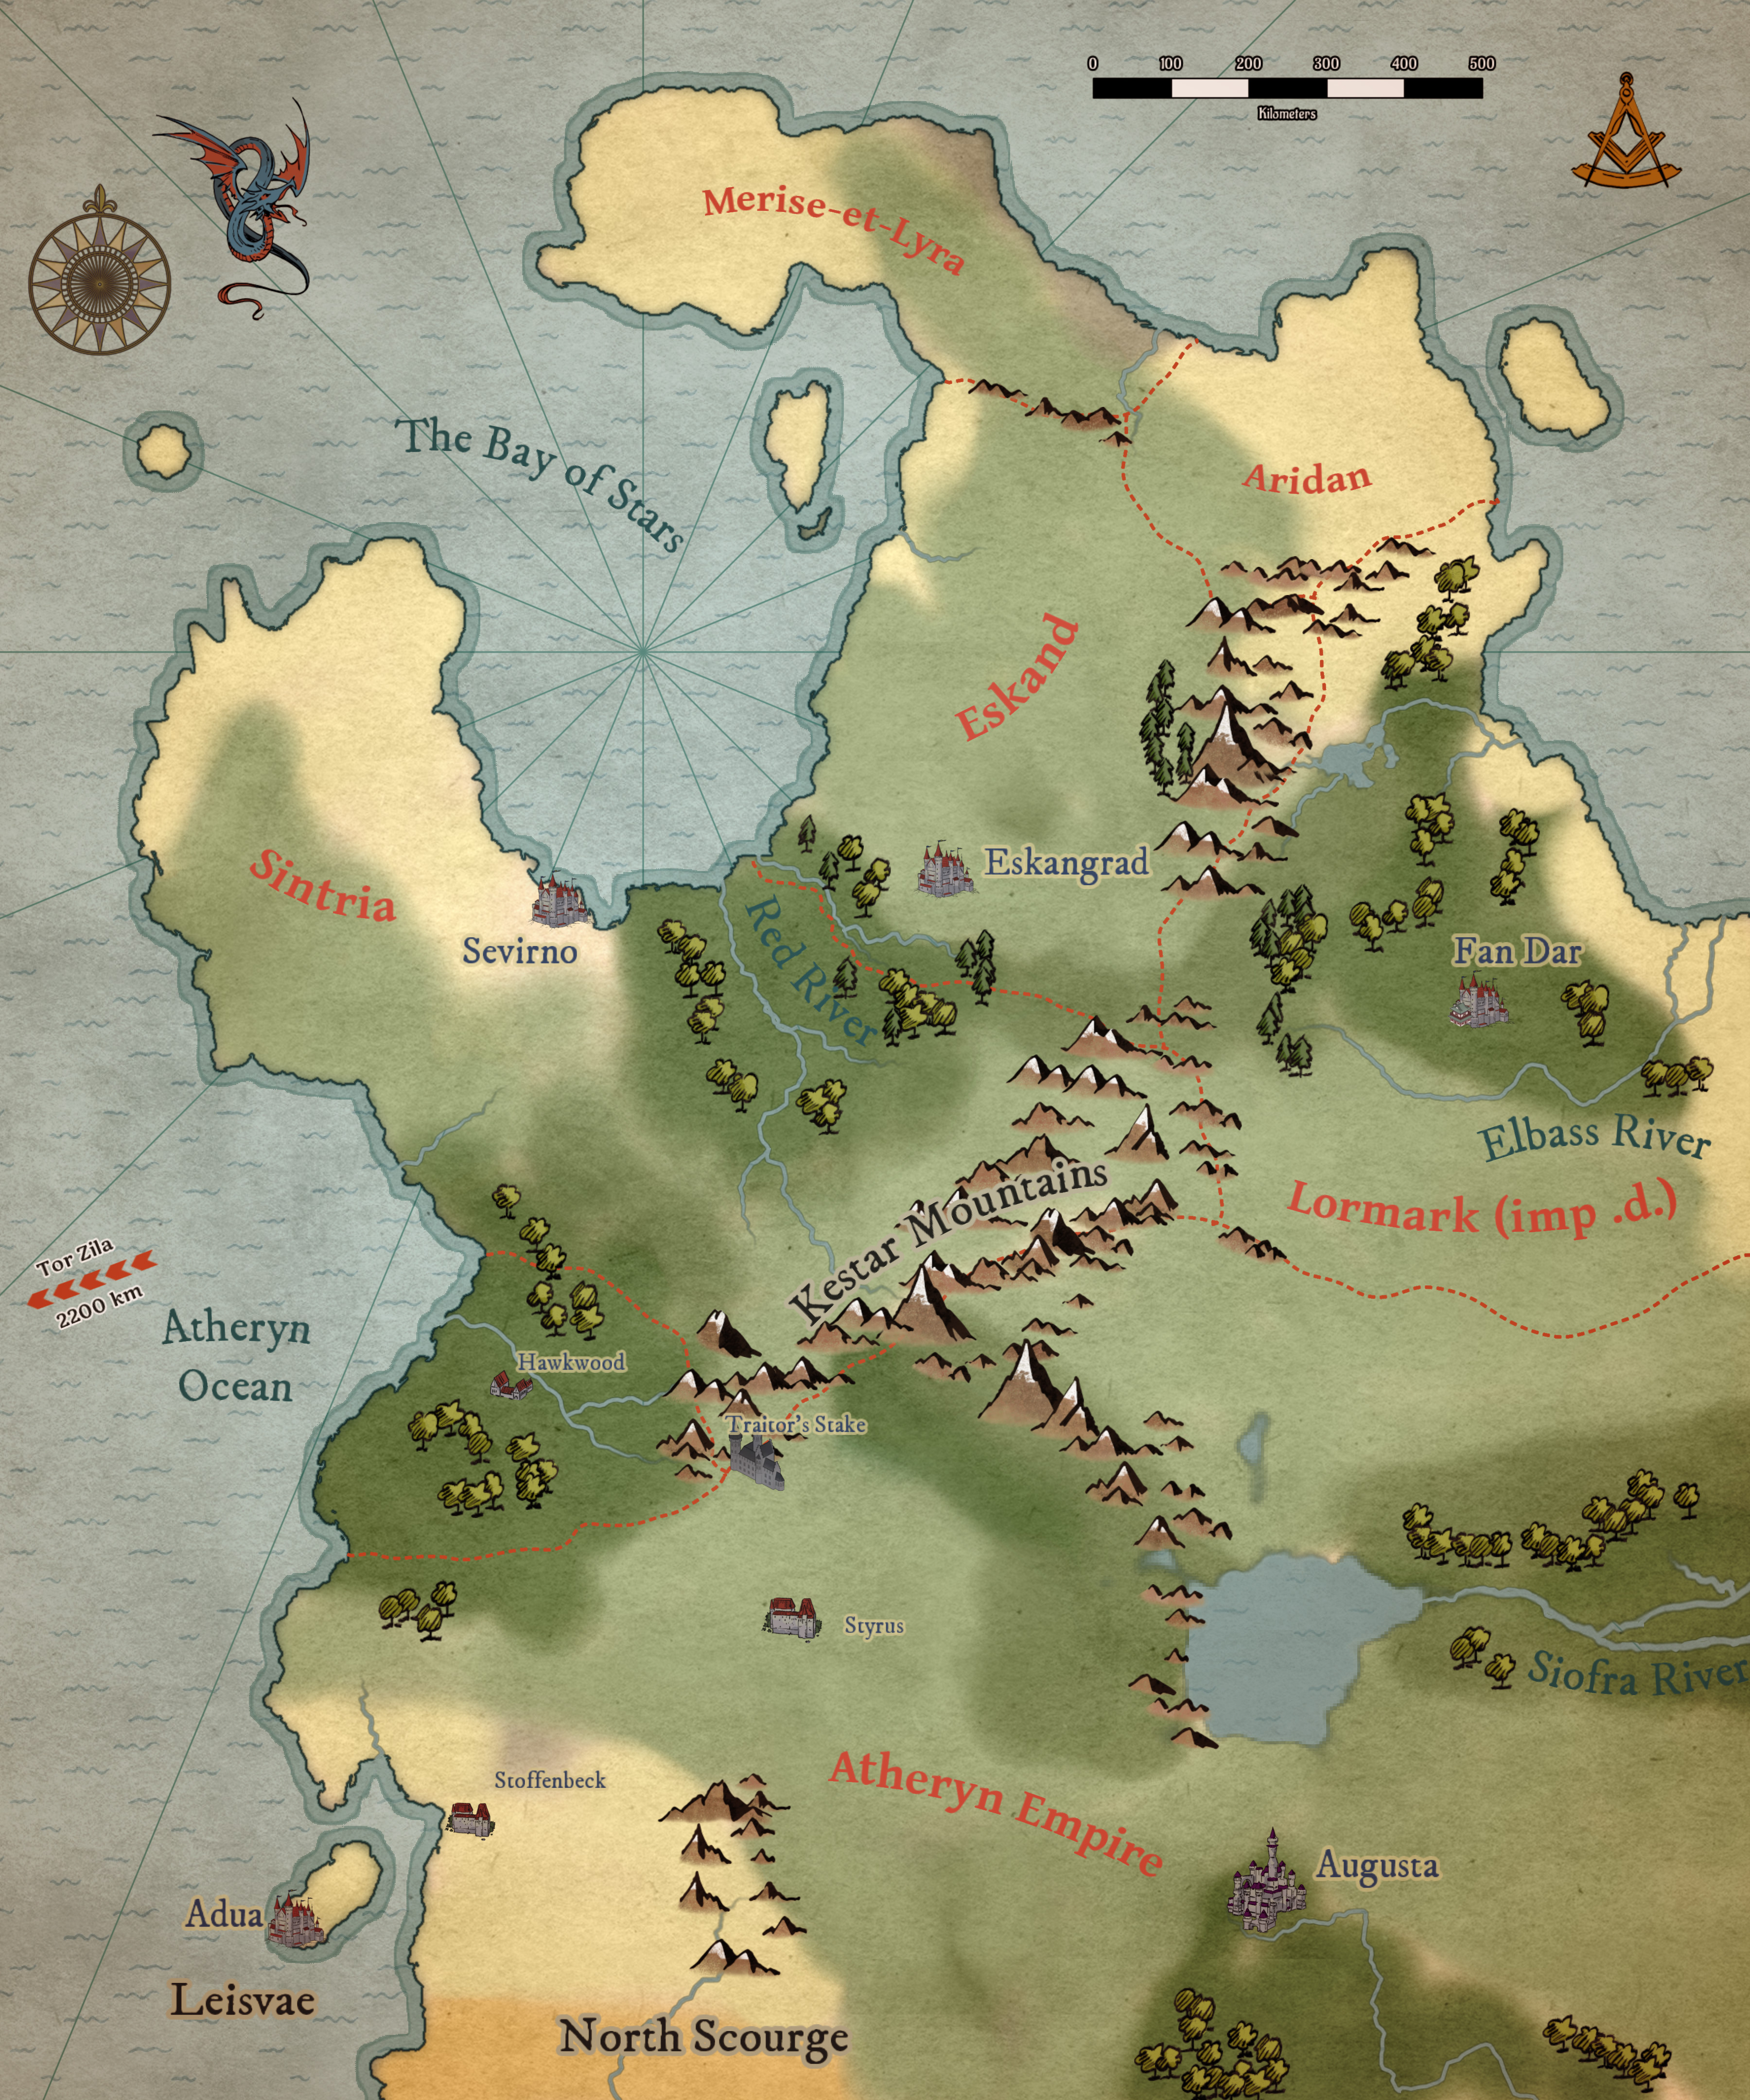
\includegraphics[angle=0,origin=c]{img/map_main_continent.jpg}
    }
    \caption{Map of the Eastern Realms, on the north of the Continent. Only major settlements and realms are represented. "Imp. d." stands for "Imperial dominion".}
    \label{map_2}
\end{figure*}



\subsection{Dreamshard Archipelago}

The Dreamshard Archipelago contains many large islands, some of which are contested by several parties. Its geography is presented on Map \ref{map_1}. It has a diameter of roughly 1800 kilometers, and its eastern edge is located about 2200 km from the western edge of the main Continent. As such, travel between the two takes about two weeks on average, depending on the weather.

The largest island of the archipelago is home to Port Darla, its greatest and msot important city. The secon largest island, to the northeast, constitutes the homelands of the realm of Hereroq. There are many smaller islands, including the warm and volcanic Isla Faris to the southeast, and the fertile island of Providence to the west.

Owing to its size, the Dreamshard covers a breadth of latitudes, and as such virtually every climate can be found within. That being said, the most widespread biome is similar to the Mediterranean climate in the real world: warm, with occasional dryness (especially in the southwest). However, the southern islands have a hot tropical climate, milder climates are found in the north, and many mountain ranges are high enough to have a cold climate.

The archipelago in rich in many important resources. Most are mainly of commercial interest, like spices and olives. But the Isles are also also particularly rich in tellurium, a metal critical to industrial applications of Magic.

Historically, the archipel has been settled for a long time. But it has seen renewed attention recently, with the latest wave of settlements (from the IDC, FSN, etc.) beginning only roughly a century and a half ago. It was justified, on paper at least, by the pursuit of old \textit{de jure} territorial claims. Even so, the polities of the archipelago remained a distant second fiddle in world affairs, until an uptick in the rate of discovery of Voskari artifacts resulted in a regain of interest and thus a settlement rush, 75 years ago.



\subsubsection{Port Darla}

Port Darla is a boom town, and contains headquarters of the Imperial Dreamshard Coumpany. It was founded by Francis Darla 62 years ago, with Lucius Clarence arriving as governor 4 years ago. 


\begin{rpg-quotebox}
    The advantage of having deep pockets? You can bury your opponents with their contents. \\ \textendash \textit{Lucius Clarence}
    \end{rpg-quotebox}
 
It has become an important city of thirty five thousand inhabitants, mostly funded by commerce incidental to the Dreamshard Rush. As a new city, it was built according to a geometric plan, with four main avenues corresponding to cardinal points.


\subsection{Eastern Realms}

The main continent, presented on Map \ref{map_2}, is home to several polities. It is often referred by its inhabitants simply as "the Continent", capitalized, in an amusing display of chauvinism. It is indeed large, even when only considering its northern part: the distance between Sevirno and Augusta is roughly 1600 km in a straight line.

The most notable polities of the Continent are: the powerful Atheryn Empire, the independant Northern Kingdoms, and the semi-independant Lormark valley. It has a temperate cold climate to the north of the Kestar mountains, while the south has a warmer climate.

The extreme south and east of this continent, which are not depicted on the map, remain only partially explored by the aformentioned polities. As such, they are improprely called the Uncharted Lands\footnote{In concept, this is a blank canvas for players to propose any origin concept they want, in accordance with the GM.}. They include (but are not limited to) the Scourge, a dry steppe full of aggressive cultures; This separates the so-called Eastern Realms from other advanced civilisations on the two other continents, because it lengthens the required sea travel as there are fewer safe harbors.

\section{Cosmogony}

The planet is a sphere, has one moon called Sela, and orbits a yellow sun simply called Sol. Known planets in the solar system include Lyria and Aulcus, and known constellations visible from the Dreamshard include the Chimera and the High Cross, which contains the Polar Star.

In the classical Atheryn Imperial calendar, used in the Northern Hemisphere, the year begins with spring and is divided in 12 months (Germinal, Bloomal, Landfall, Messydor, Sundary, Fructider, Vendemare, Brumare, Frosmare, Snowfall, Rainfall, Windfall) of 30 days each, plus an "out-of-calendar" week that celebrates the end of winter and the beginning of spring for this hemisphere. The first year of the calendar is the day of the founding of Augusta, the imperial capital. \textit{The current date is 18 Vendemare, 1440 A.U.C.}


\subsection{Magic}

\label{magic_lore}

Magic is a force that lets its practitioners achieve all sorts of effects, some of which bend the laws of physics as we know them in the real world. As best as anyone can tell, the existence of Magic seems to be a fundamental property of the universe. The currently prevailing theory is that sentience, in its broadest meaning, is what lets someone effect Magic.


\paragraph{Of Wizards and Magisters}

Magical potential is a combination of nature and nurture. This means that, technically, everyone can perform Magic. In practice, however, wizards are an extreme rarity\footnote{About as frequent as champion athletes, virtuoso artists, genius scientists, etc. are in the real world.}! This is because Magic is extremely difficult, and has a poor cost-to-benefit ratio for most people: it takes the average person years to learn how to conjure a small flame, while rubbing flints together is easy.  But for those with the natural capabilities (or money) to persevere, the rewards can be great. People who manage to push past the break-even point are called Wizards, with the very best being known as Magisters.


\begin{rpg-quotebox}
   The fewer people are capable of stopping you, the more powerful you are. \\ \textendash \textit{Arch Lector Merivahn}
\end{rpg-quotebox}

There exists a Magister Order which is meant, on paper, to be an association of those mighty few. But in practice, Magisters are almost completely autonomous. While collegial Institutes of Magic exist, in practice there are so few skilled Magic users that most Wizards learned through a more personal master-disciple relationship, or simply by trial and error. 

However, there are puzzling exceptions to these rules. Some people can have instinctive capabilities for Magic. Those are usually people with considerable Resolve, and in general what we would call Great People, Leaders and Heroes. For instance, consider Saint Lucien, a prominent figure in the Dawning War, which is the founding event of the Atheryn Empire. He became a powerful, if specialized, Magister with only minimal training. But he was a charismatic leader, and it was observed that his followers would often survive wounds that should have killed them. It goes without saying that this fueled intense jealousy from the Magisters.

Relatedly, the beliefs of many people, even without magical talent themselves, can still coalesce and produce magical effects or strengthen a Wizard. But in these cases, the effects are usually much more subtle. While gods do not exist in this setting, this effect led some people to see Magic as a divine gift (some believe it is from the Voskari...) or an answer to prayer, or something akin to unleashing one's "inner potential".

Parenthetically, while people with temporal power (kings, etc.) are expected to have a basic understanding of Magic, few use it themselves\footnote{Much like advanced technologies in the real world.}. Magister Kings are a terrifying sight, but since ruling can be a dangerous profession, most Magisters are content with acting as grey eminences instead of making plays for the throne.



\paragraph{On Source}

Magic is studied scientifically by some, but remains poorly understood. Tangentially, this explain the screwed-up formulation of prophecies and certain Spells: they are written by trial and error, modifying them a word at a time to see what best matches the currents of Magic. 

All the realizations discussed above led to the Source Theory of Magic: that Magic is created by \textit{sentience}, as Humans are by far the best generators of magical energy. This is done consciously by Wizards, who use their Intelligence to channel Magic; not only the magic generated by their own sentience, but also to a lesser degree channel the general "magical field" comin from the mere existence of sentient beings. The rest of mankind can do this unconsciously, but much less efficiently. There is only one flaw in this theory, but it is a major one: it appears non-sentient animals, golems, and even a barren desert will have a small but nonzero level of Source present. In fact, the cosmos itself contains endless Magic, but with minute density. No satisfactory theory currently explains why.

Raw Magic can be stored in physical form. It's usually in this form that is it called "Source", unsurprisingly. Source behaves something like a gel, but its behavior consistently defies the laws of physics. However, it is not usable as-is, and must be refined again through a Sigil to be effective.


\paragraph{The Nature of Magic}

Magic is performed through the proper Sigils, augmenting them with Accents. Each Sigil covers a certain type of effect, such as fire, healing, divination, to name a few.

The most common way to do so is by engraving or painting a Sigil on a support, with advanced inscribing requiring specialized materials and tools. Sigils can also be encoded in a vibration, such as a song, but the usual way to cast a Spell directly is by forming a Sigil through hand gestures. Experienced Wizards can be discrete and cast directly from their willpower without gestures or materials, but This is considerably more difficult. 

The main factors limiting the potential of Magic are intrinsic: Sigils and Accents must be made with daunting precision to work, and they are extremely difficult to standardize since the flow of Source is never exactly equal between two castings, even at the same position or the same time. This means that the most common way to use Magic is to use Magical Implements of pre-prepared Spells.

Indeed, some forms of technology rely on Enchanted Objects. While still rare, this is gaining popularity, but only up to an extent since this is very costly. As such, the practice has only noticeably impacted some specialized high-value industries.


Tangentially, even more potent Magic can be created by working at a more fundamental level through the Source Sigil. This is however enormously difficult and very finicky, and as such is not available to the players. It should be a "plot device" only if needed.

Based on Source Theory, it is also possible to Purge someone or something to extract their Source and strengthen Magic, but this is obviously frowned upon by most.


\paragraph{Effects and limitations}

\label{magic_effects}

While Magic can have many wondrous effects, it will remain fairly limited in scale. In particular, I would refer you to the description of the different Sigils, which is given in section \ref{abilities_list}, to get a general idea of what is possible. In this section, I will give additional clarifications.

In terms of scale, for instance, conjuring fireballs is extremely rare, and magical healing will usually be restricted to immediate knitting of the flesh and accelerating natural recovery. Magisters can be powerful, but nobody is strong enough to call down meteors or similar cataclysms. At least, that we know of... On that note, only Magisters can acheive anything really spectacular: for example, then tend to live longer, but mostly decades and not centuries\footnote{An apocryphal writing by Saint Lucien states that he ended up befriending families instead of individuals, justifying it by saying that "I befriend people I like, but sometime people change. Similarly, descendants are close but not quite their forebearers. I see no meaningful difference in either evolution."}.

Prescience through Divination is possible, but the usual form is simply a predictive algorithm that taps into the subconscious computing power of the caster's mind. Extralucid perception is however possible, by using this Sigil to talk to animals, in other languages, and for remote communications (although such long distance communications are difficulty and reserved for essential messages).

Sigils such as Nature or Summoning may be used for limited metamorphosis and mutagenic purposes, but any use of Summoning will have very impermanent results, as conjuration of physical matter out of nothing is extremely limited. It is also possible to be creative: for example, Telluric and Force have many engineering applications.

On the end of the spectrum, it should be noted that manipulating fundamental properties of space-time, the cosmos, and creating new planes of existence are all theoreticaly possible with the Source Sigil, the immense amounts of power required are well out of reach. For the moment, at least...

\paragraph{Echos}

Echos are remnants of sentient beings, a magical fac-simile created by the residual impact of their sentience. They manifest as disembodied ghosts. Echos can physically affect the real world in the world, but are usually very weak, unstable and nowhere near as smart as the alive person. When someone is still alive, their Echo does not manifest as it is (usually....) drowned out by the footprint of their current self\footnote{Incidentally, some random Echos found in the Aetheral suggest the existence of other sapient species far away, perhaps on another plane of existence. At least some of those Echos could be from our Earth, could they not?}.

There are three cumulative factors that strengthen an Echo: having a high Resole in life, being talented at Magic, or simply being manually "infused" magically in the proper way (although this is a risky and failure-prone procedure).

\begin{rpg-quotebox}
    From across time and space, they will answer the call. \\ \textendash \textit{Arch Lector Merivahn}
\end{rpg-quotebox}
        
Views on Echo manipulation views. Generally, people with a favorable view of Magic (mainly the Atheyn Empire and Lormark) will be open-minded. The others will be split between awe and wariness.




\subsection{Bestiary}

Most living species from the real world also exist here. There are, however, more than a few additions.

\rpgart{t}{img/art/kelp}


\subsubsection{Synthetics}

Any creature brought into being through artificial means (read: Magic) is called a Synthetic, often shortened to "Synth".

Magic can be a powerful mutagen. This means someone talented and determined enough can create truly screwed-up monstrosities. But creating something stable, or that can somewhat find its place in an ecosystem, both requires great power and great knowledge. 

Another drive behid the creation of Synthetics is that they can act as mataphysical Source reserve vats. As such, it should be noted that all Synthetics, without exception, have an intense craving for Source and Magic in all its forms.

As the fallout from many Voskari findings can attest, an uncontrolled release of Magic can also have this kind of effect.

As the voskari fallout attests, ambient uncontrolled release of magic being released can have this effect, introducing controlled or uncontrolled mutations 







\footnote{Genes can be selected for, creating specific family lines, epigenomics nonwitstanding. Indeed, Magisters are particulary adept at eugenics.}. \footnote{While natural evolution takes millenia, although microevolution of small characteristics can be done over a few generations (depending on generational speed)}


\footnote{Quadrupeds will generally share a bone structure and muscle attachments, traces of which can be seen in fish even. Muscle attachments for the face are cheekbones and lower far mandible (although scapula have different angles and first joint is closer to body, also share muzzle extrusion but with differing shapes ofc), beyond that chordata. Magic can be used to SPEED ALL OF THIS UP CONSIDERABLY.}


\paragraph{Constructs}


An important other aspect is the existence of Constructs, aka. golem and robots animated by magic, which are also technically "Synths". They can be partially organic or sometimes even fully inorganic. While those remain difficult to manufacture and hence rarely used, they are efficient calculators and can sometimes have some modest level of sentience. As such, those constructs are used to analyse large amounts of data and to perform hard labor. 


A philosphical dilemma is currently brewing on what moral status they should have.
Two other dilemmas : they are improving quicky and could conceivabley become fully sentient. As such, could they become wizards ? It is argued that their brand of sentience is focused on different applications, more specialized but dumber, compared to humans' and they are not focused on imitating humans but on high level mathematics, so this is uncertain. This is mere speculation. For now, at least... besides, artificial biological sapients are at least possible in principle, if rare :








\paragraph{Synthetic sapients}

The only naturally sapient race are Humans. Other sentients beings are so rare as to be anecdotal, and all of them are either whole-cloth Magical creations or simply magically-altered humans. 


Constructs are not sapient as we mentioned before, but the future is unclear.


\footnote{Artificial sapients are limited by the same biological constraints (brain maturation, etc.). Also, owing to the nature of their creation, they often have very unstable genomes (in the sense of containing many deleterious mutations and sometimes uneven numbers of chromosomes) ; as such, they are usually sterile or at least infertile.}



\footnote{Some Magisters even manufactured anthropomorphic human-animal hybrids for... sordid purposes.}


















\subsubsection{Menagerie}

- Elephants and camels somewhere, in addition to cavalry (off handedly mention all three species being indigenous to Dreamshard, albeit in different biomes)
- Put in some dinosaurs in a lost island ! (conserved magically ?) they also conveniently explain some "monstrous" creatures, just like IRL !

Off handedly mention that many of them can map to existing Bestiary profiles with only minor adjustments


Among the menagerie: to be spread into the relevant sections above when discussing them


\paragraph{Horrors}

- Animated trees
- Bismuth/tellurium golem
- Enthralling fungus
- Drowned ones
- Kraken (created)
- Arachnoid experiment
- Animated armor/Golem
- Drillworm? very large worm-ish thing
- Bone Bishop
- Drake purger
- Ashmen
 - Ghosts/echos
- "Demons" which are the result of Voskari experiments:	MANY, MANY fucked up Giger-esque Voskari-created monstrosities (ashmen included, and giger-esque machine tyrants) –> mentioned as "rumors"
- Constructs : golems, replicas
- Avatars: lupine anger, or avatars of strong emotions, works a bit like chaos demons in Warhammer 40k, and are close to Echos in their principle.

\paragraph{Success stories}



- There are however examples of artificial species that found an ecological niche. THey remain rare due to their craving for Source, but they exist nonetheless. 
	Shuddaka : trees with blue leaves and silver trunk, caused by the presence of actual silver, with communicating roots
	giant pillars-like coral formations
	coastal algae srpouting into the air thanks to air balloons
	monkey with a collar of sort of tentalcles for better prehension
	horses with boney crest for muscle attachment for additional strength
	large (mammoth-sized) animals with a flock of supporting organisms, killfish style
	basaltic organs are a must have! Idea: have some gradually slit tout, like missiles launching, and then explode in the air
	catlike species with very elastic tendons, can bend its spine into nighmarish contortions
	bird with mirror-like scales (yeah... I know) it can rotate while flying to reflect light or distract predactors
... as for size show a little of everything. i don't think i will go all the way up to something like massive dinosaurs, maybe one or two representants of almost extinct species, or an Abomination.






































\section{People and Cultures}

The world contains a variety of peoples and cultures, organized in a breadth of nations and polities. We will present those relevant to our story in this section.


In brief: the Eastern Realms, which designates the nations of the central Continent including the Atheryn Empire, have... heavily invested, shall we say, in the Dreamshard Archipelago recently. This, understandably, made the local potentates wary and had led to a sequence of portentous events. We will detail those later in section \ref{recent_history}).






- Describe skin tone and physical appearance of the peoples in their respective sections. Hereroq should be brown, lormark a bit more east-asian-ish but with high diversity, empire is mediterranean, north is european, find a bit more (notably there are blacks far to the south in a southern continent beyond the sand scourge, much like there is likely an eastern continent with asian-ish and brown-ish people







\subsection{Factions and History}

\begin{figure}[!ht]
    \centering      
        
\includegraphics[scale=0.25]{img/flag/atheryn.png}
        
\includegraphics[scale=0.25]{img/flag/eskand.png}
        
\includegraphics[scale=0.25]{img/flag/fnc.png}
        
\includegraphics[scale=0.25]{img/flag/fsn.png}
        
\includegraphics[scale=0.25]{img/flag/hereroq.png}
        
\includegraphics[scale=0.25]{img/flag/idc.png}
        
\includegraphics[scale=0.25]{img/flag/locals.png}
        
\includegraphics[scale=0.25]{img/flag/lormark.png}
        
\includegraphics[scale=0.25]{img/flag/sintria.png}
        
\includegraphics[scale=0.25]{img/flag/voskari.png}

    \caption{Flags of respectively, in classical reading order (left to right on each successive line, then moving in lines from top to bottom): the Atheryn Empire, Eskand, the First Northern Company, the Free Sailors Nation, Hereroq, the Imperial Dreamshard Company, the local Dreamshard dukedoms, Lormark, Sintria, the Voskari.}
    \label{flags}
\end{figure}








\subsubsection{Atheryn Empire}


A powerful empire ruling over the central part of the main Continent.


\textit{Leader}: Emperor Varen I Atheryn.

\textit{Population}: estimated 40 to 60 million inhabitants, 10 or more additional million with dependencies).

\textit{Wealth per capita}: Moderate on average, but with significant inequalities between the very rich elite class, and a considerable poor underclass. For dominions and dependencies, it is very variable.

\textit{Territory}: Most of the center of the Continent, with its capital at Augusta.
    
\textit{Colors}: Purple (major), white and black.


\begin{rpg-quotebox}
They say we make a desert and call it peace. I say we shatter so we can rebuild. \\ \textendash \textit{Gaël Valens-Détianne}
\end{rpg-quotebox}

The Atheryn Empire was founded by Saint Lucien in the Dawning War, which we mentioned previously. Their architecture style would best be described as neo-classical by the standards of the real world: they are very fond of columns and amphitheaters).

The Atheryn have grandiose ideas of what an Empire should be, straight out of the real-world Antiquity. The Atheryn believe they have been invested by the "Fates" of a grand civilizing mission, to bring the light of their culture, spread the "benefits" of their Empire to the entire world. As such, while they are somewhat racist, it is more of a cultural supremacism: they will embrace local converts and favor syncretism, as long as the resulting mix is more Atheryn than not, of course. On the flip side, defiance is met with brutal repression. 

Predictably, their political system is very backstabby. Although there is an Imperial Senate, senatorial mandates are very long, and suffrage is restricted to full Imperial citizens, making the system closer to an oligarchy than a democracy. That being said, as the Atheryn believe in their universalist principles, there are possible paths to citizenship.

As a result of this system, power tends to cluster in the hands of the Great Families of the Empire, including the <PUT NAMES HERE>. Unsurprisingly, they tend to be at loggerheads with each other. While open warfare is no longer the norm, they often employ covert operatives dubbed the Skitari. They are used against each other, and sometimes even against external threats, for a change.

It should be noted that despite the preponderence of Famillies, individuals can rise to power and found new Families themselves, inclusing by adoptiopn.
Despite Families individuals can rise, Caesar or Octavian style, and found families, inclusing by adoption
This makes it more meritocratic, as titles are not necessarily hereditary (in practice, heirs offten carry on, but despite all this oligarchy and heredity,  bureaucracy is powerful and often complicates the schemes of those above. It is not unheard of for bureaucrats to carve a sizable power base.

The Empire likes magic. Magisters are often cornerstones of the power structures and families. Indeed, the current Emperor, Varen Atheryn, is a skilled Magister, who poured funds into Apocrypha : university at Augusta, capital of the empire. While the Empire is very scientistic (not a misspelling, I mean they are attached to sciene) there is a not-insignificant part of the pop that sees the Voskari as demigods and worships them, causing some internal tensions. 


While the empire is the largest nation in the world, and regroups at present a good 25-30 percent of the planet's population, not all that population has the same culture. The Atheryn heatlands have exported the Atheryn language, administration, and a bit of their culture, but syncretism remains the order of the day in the empire, and ensures its relative stability. The Empire has vassal states and duchies with tenuous control, such as Lormark, or Leisvae island, a major commercial and tellurium mining centre, ruled by House Heim, recently suffering an attempted invasion by Eskand. (<-- this is mimbraine's imperial name, tell it to flo)


The Empire's fortunes have waxed and waned over the past millenia. The northern kingdoms of Sintria and Eskand broke off a good century or two ago. The Atheryn empire has recently suffered a rather large civil war, Vakir's rebellion (Vakir was Sintrian in origin) Now that Varen Atheryn has ramassé les dents of the Empire, it looks outwards again.  no internal wars in the empire now since it's done ramasser ses dents. See recent evets. Some famous regiments include 1st 'Black Cross', 7th 'Devil's Heart' and the 11th 'Chimera'

It should be noted that most of the Dreamshard is a \textit{de jure} part of the Empire, owing to early expeditions and treaties that are now centuries old and nobody cares about anymore except for paper-thin -- literally -- justifications, but it had attracted little interest and the locals were left to their own devices. Until now.



\paragraph{Imperial Dreamshard Company}

Short summary.

\textit{Leader}: Governor Lucius Clarence (it's complicated...)

\textit{Population}: 20K employees + 1.2 million Eastern colonists growing fast, plus a few million locals in the administered territories

\textit{Wealth per capita}: Moderate, but quickly improving.

\textit{Territory}: Port Darla and many isles

\textit{Colors}: Blue (major) and white (minor)


\begin{rpg-quotebox}
    "We shall bring civilization. Through the end of a musket, if need be."
    \end{rpg-quotebox}
    



The Imperial Dreamshard company, or IDC for short, is an ostensibly mercantile company founded under the authority of the the Atheryn Empire, of which most of the Dremshard Isles are a *de jure* part.

In practice, however, they behave more like conquerors. They are resolutely expansionist, and use their large fleet to assert their influence in the archipelago. They also take an active interest in the magical phenomena affecting the archipelago.

As an extensino of the Atheyn philosophy, many colonists have come settle the Dreamshard.


Note that The Imperial Dreamshard Company and FNC below are not simply extensions of their parent countries, they have some autonomy and disagreements with the mainland. Indeed, there is some politicking between Clarence the appointed governor who is a career bureaucrat, and Savian Détianne the Adjunct Minister in charge who got the job through connections



\subsubsection{Northern Kingdoms}

The two most noteworthy Northern Kingdoms are Eskand and Sintria. There are a handful of other smaller ones (see the map), but they are almost all in the sphere of influence of the big two. Usually Feudal, with heredity of titles, and a pyramid of nobles and no suffrage.

\paragraph{Eskand}


Short summary.


\textit{Leader}: King Harmach I (de jure, in exile), Lady Sofia Valskaya (de facto)

\textit{Population}: 6 million (uncertain due to recent troubles)

\textit{Wealth per capita}: Low, partly due to recent troubles.

\textit{Territory}: a
    
\textit{Colors}: Red (major), white and black


\begin{rpg-quotebox}
Quote \\ \textendash \textit{Source}
\end{rpg-quotebox}


Somewhat more rustic than its southern neighbors, Eskand used to be a junior partner in a personal union with Sintria under King Casamir III. Broke free 80 years ago, and has been in an uneasy peace with them, dotted with low-intensity wars under a variety of pretexts.
    

Architecture would be best described as brick gothic (use those exact terms)



Sofia Valskaya recently led a peasant rebellion that forced the king to abdicate in favor of noble who is a puppet of sofia. See recent events in the red dawn



\paragraph{Sintria}

Short summary.

\textit{Leader}: Leto III Seinfeld

\textit{Population}: 11 million

\textit{Wealth per capita}: Moderate.

\textit{Territory}: a
    
\textit{Colors}: Yellow and white


\begin{rpg-quotebox}
    Quote \\ \textendash \textit{Source}
    \end{rpg-quotebox}


Cultural offshoot of the Atheryn, was a province three centuries ago but now independant. Some, but not much, hard feelings as a result. What really kicked tensions however is tha fact that Vakir (from the last imperial civil war) was Sintrian, hence tensions.

Architecture would be best described as modernized romanesque (renaissance)

They have been expansionnist, lately, both diplomatically and forcefully. The Empire worries they are trying to create a local sphere of influence that encompasses all the Northern Kingdoms.

As w would-be hegemon, Leto is weary of the developments in Eskand and is contemplating an expedition.
Sofia valskaya is secretly his illegiimate daughter, which complicates matters... see more in recent events in the red dawn



\paragraph{First Northern Company}


Short summary.

\textit{Leader}: Director Alaria

\textit{Population}: approx. 15K employees + 750K colonists, growing, plus the locals in the administered territories

\textit{Wealth per capita}: High.

\textit{Territory}: Providence
    
\textit{Colors}: Red and green


\begin{rpg-quotebox}
"Enriching mankind and enriching oneself are not mutually exclusive goals."
\end{rpg-quotebox}


In the Dreamshard. Sponsored by Sintria and Eskand mainly, but also significant participation from merchants from Lormark (see below).  
The FRC is not simply extensions of their parent countries, they have some autonomy and disagreements with the mainland, much like the IDC


They seek Profit, profit, and perhaps even more profit. Relatedly, there are averse to interventionism and military adventurism ; their philosophy instead centers around establihsing trading posts as opposed to very large scale settlements.

Several Houses (close but not equivalent to families, in that it's not necessarily united by blood) vie for control of company interests.



\subsubsection{Lormark}

Short summary.

\textit{Leader}: Confederacy of city-states

\textit{Population}: 9 million, wealthier than average

\textit{Wealth per capita}: High, significant bourgeoisie.

\textit{Territory}: a
    
\textit{Colors}: Green and blue


\begin{rpg-quotebox}
Quote \\ \textendash \textit{Source}
\end{rpg-quotebox}

On paper, the Lormarkian principalties are grouped together as the Dominion of Lormark, which is a vassal of the Atheryn empire. However, the Empire takes a pretty lax approach and leaves them much autonomy, as long as they pay their taxes. Sometimes, they even remain in practice neutral in some imperial wars (although they join on paper). 

They are commerce focused, and are also an important cetner for the study of magic.

They have been known to wage the occasional low-intensity war between each other, though Imperial authority and the necessities of business usually demands an end to those quickly.

culture is  VERY cosmopolitan, and heavily influenced (founded ?) by foreigners. Architecture contains pagodas and stupas (use those terms I think) Due to being founded by settlers and merchant foreigners from the most eastern continent (and a few from the southern) and hybridizig with local cultures


The current emperor (Varen) is seeking to turn them into a unified puppet state with tighter control, which is not sitting well with them.

	

\subsubsection{Voskari}

Short summary.


\textit{Leader}: Arch Lector Merivahn, supposedly

\textit{Population}: Unknown. Likely select.

\textit{Wealth per capita}: Unknown. Likely spectacular.

\textit{Territory}: Unknown
    
\textit{Colors}: Black (major) and yellow


\begin{rpg-quotebox}
	"Is gratitude still germane when directed at the wrong person ?"
\end{rpg-quotebox}

A riddle wrapped in a mystery. Only few artifiacts of them have been found, but findings are accelerating. The only tangible facts are the artifacts that share a common style and language. They share the Atheryn alphabet, but have their own language. Recognizable 19th-century stylistic elements mark them.

Artifacts belong to them about 10-20 years ahead of the current magical-technological level (not fantastically ahead, but quite advanced). The odd part is that this 10-20 years tech gap has remained constant ever since findings have begun, leading to speculation that they are still active and not an extinct civilization or an extinct Magister branch, and that they continue improving. One recurrent name : Merivahn.


If you buy into the most common theories, and according to some anecdotal evidence, here is the best state of knowledge: 
    - They are a world-domination Illuminati-ish secret society first and foremost. Speculated to be an ancestor or a splinter branch of the Magister Order (since magic is effective). Speculated also to be behind many weird magical phenomena recently observed.
    - external recruitment is possible from outside the organisation even though inside recruitment is preferred, and the total number of voskari Magisters is rather limited. Defections from the Voskari have happened, but the Voskari disinformation game is strong so people don't generally believe the defectors and stick to their own pet theory
    - There are two subfactions : the White and the Reds. They have competing visions for the future, and this War in Heaven is a heavy plot points. The exact nature of these competing visions is left for the reader-GM to decide.

Best we can tell, They are Humans, but that does not stop the fact that they are worshipped as mythical demi-gods in certain places. In fact The voskari religion (meaning cult that worships voskaris) is widespread and organized, which can generate religious tensions. They believe the leftover Voskari artifacts are "gifts" to mankind, to put us "on the right path". 


\subsubsection{Hereroq}


Short summary.


\textit{Leader}: Queen (closest corresponding title in Atheryn language) Hesria

\textit{Population}: estimated 14 million

\textit{Wealth per capita}: Low, but slowly improving.

\textit{Territory}: Tor Zila, Seahearth, all Isle of Hereroq and other dependencies.
    
\textit{Colors}: Beige and orange.


\begin{rpg-quotebox}
    "When the winds are changing, one must steer or die." \\ \textendash \textit{Hesria}
\end{rpg-quotebox}


The most noteworthy inhabitants of the Northern Dreamshard. A relatively large realm, controlling about half the total population and GDP of the Dreamshard Archipelago. While they shake hands with the Companies for now, the peace is tense and the Companies' outposts, including some of which are in Hereroq's dependencies, make the situation uneasy.


They are slightly backwards technologically compared to the Eastern Realms, but only slightly. Instead, their worst weakness is that they lack the wealth and especially the single-minded purpose of the Companies, which are attempting to extract concessions, buy shares in their economy, make "unequal treaties", ... and conquer what they cannot buy. They will need to play their cards rights in the coming storm. 

use some Moorish architecture too. mix of Turkic, Moorish and Mesoamerican features, with pyramids and large roof overhands (don't say ottoman and meso, say things like ("pointed arches for doors and columns, domes maybe (but many small domes instead of big ones, to be distinct), sandstone-ish, and meso-style pyramids with cyclopean blocks for religious purposes, maybe use the word "real-world moorish"))"

Notables are named the Sifs, which are member of un upper social class that is starting to diverge from the rest of the people. Politically, this is a federation: They are somewhat decentralized, with the Sifs ruling locally. Queen Hesria is looking to centralize more and reform to stand against the other Great Powers. Membership to the Sifs' social class is inherited, though, but it is reasonably frequent for rich or influential people to be named Sifs by the queen or by prominent Sifs. Also, culturally there is a 'right to rebellion', and for certain positions they have suffrage but it is censitaire. This means their values are somewhat meritocratic, but their social structure makes them quite traditionalistic and reactionary, and political corruption is a problem.

Religion is important (though the voskari cult is proportionally less important here than in the Eastern Realms, local traditions keep a better foothold), and self-sacrifice as well is a national virtue. Anecdote : they have a few temples with wings that are periodically rebuilt facing another direction, to symbolize the passing of time.

Strong tradition of naval exploration (they initiated contact with the main continent way back when, not the other way around) but don't really care for expansionnism, their last outposts have been taken over, first by the local dukedoms decades ago, and now by company encroachment (both by buying out, simply resettling them, and a few low-intensity wars). Trading posts of theirs, however, remain throughout the Dreamshard, and a handful on the Eastern continent. Importantly, they have a reputation for spycraft / being excellent spies.



Bayaz powerful magister comes from here


\subsubsection{Free Sailors Nation}

Short summary.

\textit{Leader}: "Admiral" Veraume

\textit{Population}: approx. 10K sailors, + locals

\textit{Wealth per capita}: Moderate, but only in fungible and not productive assets.

\textit{Territory}: Smuggletown
    
\textit{Colors}: Green (major) and teal

\begin{rpg-quotebox}
    "Let the empires bicker. We'll be there, quietly waiting to bleed them dry." \\ \textendash \textit{Source}
\end{rpg-quotebox}


Pirates operating almost exclusively in the Dreamshard. Sometimes, some among their numbers sell their services as privateers. Some Asian-ish elements (junks, came as some early leaders were fleeing from the asian-ish lands and brought those ideas, and catamarans from ancient natives for scouting and messages) but very patchwork. 
	
Your garden-variety pirate nation, loyal to no one but themselves, seeking profit above all else. Open to taking privateer jobs. They are not, however, bloodthirsty thugs, but attempts to form an organized nation have been met with defiance from within.




\subsubsection{Local Dreamshard petty realms}


Short summary

\textit{Leader}: Various

\textit{Population}: Unknown, estimated at several million in total spread across the archipelago

\textit{Wealth per capita}: Low.

\textit{Territory}: Anywhere in the Dreamshard not (yet) claimed by any previously mentioned Great Power.
    
\textit{Colors}: a

\begin{rpg-quotebox}
    Sleepless nights are very good at reminding you about all you have to lose. \\ \textendash \textit{Who Said It}
\end{rpg-quotebox}

Besides the great powers, there are local dukedoms native to the isle, with wooden eastern european architecture. 
Many of them come from peaceful mixing between the "ancient natives" (see below) and very old progressive settlements from the Eastern Realms (who had some parts of dreamshard as de jure) ; however, their relative isolation led to cultural divergence, and today they are more like estranged cousins than brothers of the Easterners, especially with the mixing with the natives



Those dukedoms have intermediate level of tech, and relations with the Great Powers are tense because of encroachment. Alliances and low-level warfare between them sometimes, very shifting.
	Duchy names : Berus, Senria, add a third one

\subsubsection{Others}

There are scores of other people, big and small, that make up the Circle of the World.

Of note, we have:

- Ancient Natives of the dreamshard: pastoral, half-sedentary and half-nomadic (some tribes are only sedentary or nomadic while some alternatate ), with Chiefs that are a primus-inter-pares things and the influence of Druids/Shaman (dependin on translation), and the importance of Prestige. Skilled at raising camels and elephants for those living in the extreme south, while the northern ones are more often nomadic with horses or guerilla hiding in the forests, and the center ones have some wooden architecture. They are pretty much a spent force, have begun mixing in with the local dukedoms, particularly wiuth hereroq and now with the empire. Of no further consequence.

- Uncharted Lands are a border of the empire, like the limes in real life.
The Scourge is on the south of the main continents. Some parts are steppe, some parts are a dry dusty desert. Home to Steppe nomads.







\subsection{Local life}


\rpgart{t}{img/art/island}

The specificities of the culture of each faction have been mostly introduced in the previous section. Some additional considerations are presented here.

\paragraph{Languages}

The Atheryn language is a global \textit{lingua franca}, although it comes in a large variety of dialects, those are usually mutually intelligble. In particular, the languages spoken in the Northern Kingdoms are heavily influenced by it. Otherwise each culture has its own language.

\paragraph{Currency}

The money of the Atheryn Empire is the gold 'mark', subdivided in silver 'aces' and copper 'pennies', as stated in the rules. Ten pennies are worth an ace, and ten aces are worth a mark. Instead of marks, the North (and the FNC by extension) uses 'florens', and the Hereroqis uses 'denirs' which is often bastardized to 'deniers' by Easterners. All three have roughly equivalent value, and are generally seen as strong currency and accepted around the world.


\subsubsection{Technology}

The technological level is roughly equivalent to the Early Modern real world in Eurasia, outside of magic of course. with arquebus (in terms of philosophy, of course the presence of magic changes much) with forays into 18th century modern theories (or magical equivalents) but only rarely.


\begin{rpg-quotebox}
    Oh, we are way past 'unreasonable'. In fact, I'd say we crossed the line into 'insane' a while ago already. \\ \textendash \textit{Who Said It}
\end{rpg-quotebox}

proto-industrial revolution in the empire and the north with manufactures. As mentioned before, enchanted objects and magic have made in impact in some high-tech industries and there are applications, but it's very niche.

The best (often Voskari, but NOT EXCLUSIVELY! important to say Voskari do not have a monopoly on high-tech !!) can create some interesting stuff, which is partly technology and partly magical, but do recall that magic is studied by some people as a science so the frontier between the two can get blurry.



This includes, but is not limited to : primitive submarines, flying carpets, "omnicalculators" (often used to predict outcomes), magnetic rifles
Most of those, however, are limited series and prototypes. For now, at least...
- Needle gun (breechloader)
- Liquid breathing
- Enchanting, machine learning, 
- receptacle of energy upon a creature, to improve it ?
- Gateway/warp drive/wormhole ? Unsure





\subsubsection{Customs}

But also Tyranny antiquity-like "grandeur" and neoclassical thrown in for the Empire mostly

When it comes to what we would call today "progressiveness", meaning concepts such as female soldiers, homosexuality, and general acceptance, this world is arguably somewhere between the IRL Middle Ages in the Mediterranean, and today's Western societies. While opinions will of course vary by cultrure, in most of the world all of the above will be seen as "eccentricities", enough to stain a reputation but not sufficient to make someone a social pariah.

That being said, relations (romantic or otherwise) between social classes will be scrutinized in places where Great Families are important, and Magisters tend to be rather eugenist. Relatedly, I think a minor culture (not hereroq; likely one of the lormarkians) has castes (merchant, warrior, priest, peasant, etc.) somewhere

The Atheyrn Empire has indentured servitude, while the rest of the Eastern Realms instead use a lighter form of serfdom with potential for social mobility. Full-on chattel slavery is the exception, present only in a few polities in the world.

Furthermore the "do you not know that you are gods" religion is more popular in the north, while in the empire they have a deeper fascination with the voskari and the mystery-cults around them spring up there




Ship types:
	Like in PoE there should be Galleons and sloops, and dhows for hereroq.
	As for Junks, these are lormark based, but maybe the pirates adopted some. Same rasoning for the camataran-polynesian stuff like in pillars might be mentined in a Lormarkian background, but I am unsure it fits, perhaps pirates use them as messenger boats





\section{Recent history}

\label{recent_history}

In this section, I will present the most recent events and relevant \textit{dramatis personae}.

\subsection{Vakir's Rebellion}

The most important and portentous event in recent history is Vakir's Rebellion. Over the last century, the Atheryn Empire was experiencing a decline, which cultimated in the start of the Rebellion, 20 years ago. Vakir's Rebellion started with a dynastic pretext, and esclated when some families and even entire provinces that resented the Empire threw their lot with Karthus Vakir (who was originally Sintrian, but raised imperial, and had the backing of a portion of the army). Vakir's hold has been destroyed and is now Traitor's Stake.


\subsubsection{The Empire Strikes Back}

The Empire has now just recovered from Vakir's rebellion and is now looking outwards again. Emperor Varen Atheryn launched a reconquest of seceding territories 10 years ago that is nearing completion.

Emperor Varen Atheryn: knows magic. Held the empire together during the recent trouble, but his immediate family died in the war, so his nephew is now heir apparent. Due to this loss, Varen has grown jaded and disinterested.

One territory that escaped his notice is Leisvae. Invaded by Eskand during the rebellion, it was negelcted as the empire's resources were spent elsewhere and managed to liberate itself. Now jockeying between two factions led respectively by Caroline and Isgrin Heim, hesitating between rejoining the Empire and staying independant. Everybody awaits the empire's reaction

\subsection{The Red Dawn}

Meanwhile, in the North, a popular revolution called "Red Dawn" in Eskand led by Sofia recently deposed Eskand's king Harmach I and installed a puppet king. Leto III Seifeld of Sintria wishes to intervene. Sofia is secretly Leto's daughter and has been recorded saying that she "resents him for what he did" (unclear, assumed to have something to do with her mother). Leto is a benevolant despot, but a despot nonetheless. Tthinks he has a responsability to "make things right" for the North and build a sphere of influence for Sintira here. There is also the distinct fear that the Red Dawn could spread... which could explain Leto's motivatino to intervene.

\subsection{An Odyssey to the West}
 
Concurrently, there has been a quasi-colonization (use the word colonization !) boom in Dreamshard by all Eastern Realms over the last century, driven partly by escapism from the unstable situation in the East and by large increases in discovery of Voskari artifacts. This boom fed on itself, and now the archipelago became wealthy and valuable in and of itself, which increased its attrativeness even more.

Resulting in an uneasy political situation, as has been explained before when presenting the factions. It should be noted that many Dreamshard isles are historically fringe territories (explored and claimed on paper with sparse settlements) of many of the Eastern Realms, so they have a legitimate de jure claim, although they were negelcted backwaters until recently. This, however, has fooled precisely nobody. It is clear why exactly the settlers and the Companies are arriving (voskari artifacts, important resources, and well territory in general) and everybody knows the de jure claims are just a convenient excuse. After some diplomatic, economic, and even military skirmishing, there is now an uneasy peace between the Companies, Hereroq, and the other potentates.

\subsubsection{The City of the World's Desire}

In Port Darla : Lucius Clarence: 37yo, governor of the Imperial part of the Dreamshard Isles. Ambitious and sarcastic (rq : governor is an APPOINTEE position, he rose meritocratically here), nominated 4years ago. Lucius Clarence and the company's titular Minister (Savian Détianne) have a tense relationship as we mentioned, while Clarence is technically his supervisor, he has to negotiate sometimes to get full company backing. Mention Amelia Talborn as one of the Magisters who set up shop in Port Darla

Clarence and magister Bayaz are good friends


\subsection{A Farisian Question}

Which brings us to the most recent notable event, the eruption on Faris Island, in the Dreamshard Archipelago: pyroclastic clouds, weird sightings, suspected voskari involvement. Unexplained volcanic eruption as Isla Faris. Voskari artifacts found there. This has drawn the interest of everyone important.



---



\subsection{Some examples of names}

Don't make a list. Instead sprinkle them and mention them by name in the relevant sections about their origin cultures. say those are great families or persons of interest

A good way is to use them in the quotes

Empire > Some important people and families to name drop : Détianne, Savian, Arbuthnot, Lucius Clarence, Sabadi, Gael, Valens, Skitari ?, Berus, Zacharus, Du Bois, Talborn
HEREROQ > Some important people to name drop : Hesria, Lokdan, Nusal, Bayaz
North > Some important people and houses to name drop : Seinfeld, Val-Skaya, Anna, Mark, Talbot, Sevirno, Marda-Torai, Rieser
Lormark > Some important people and houses to name drop : Harmaak, Senria, Lu Dar, Radishaj
Voskari: Merivahn

 

\end{appendices}

\end{document}